\documentclass[draft,floatfix,prb,aps,superscriptaddress,11pt]{revtex4}
\usepackage{amsfonts}
\usepackage{amsmath}
\usepackage{graphicx}
\usepackage{showkeys}
\usepackage{ulem}
\usepackage{subfigure}
%%%%%% defs
%%%% acronimos
\def\ps{\mathrm{ps}}
\def\lda{\mathrm{LDA}}
\def\rpa{\mathrm{RPA}}
\def\nl{\mathrm{nl}}
\def\acu{Accu-Check\textsuperscript{\textregistered}~Performa}
\def\goni{Glucometro \'Optico No Invasivo}
\def\Reg{\textsuperscript{\textregistered}}
\def\tiniba{ TINIBA\textsuperscript{\textregistered}}
\def\gw{{\it GW}}
\def\gsa{Generaci\'on del Segundo Arm\'onico}
\def\shg{Second Harmonic Generation}
\def\sfg{Sum Frequency Generation}
\def\sdf{Generaci\'on de Suma de Frecuencias}
%%%%% accent of i
\def\'#1{\if#1i{\accent19\i}\else{\accent19#1}\fi}
%%%%% compa\~nias
\def\micro{{\it Supermicro}}
\def\lufac{{\it LUFAC}}
%%%%% lugares
\def\lou{Laboratorio de \'Optica Ultrar\'apida}
\def\roma{Universidad de Roma II}
\def\tor{``Tor Vergata''}
\def\dti{Direcci\'on de Tecnolog\'{\i}a e Innovaci\'on}
\def\dfa{Direcci\'on de Formaci\'on Acd\'emica}
\def\dg{Direcci\'on General}
\def\da{Direcci\'on Administrativa}
\def\ifug{Insituto de F\'isica de la U. de Guanajuato}
\def\icf{Instituto de Ciencias F\'isicas}
\def\unam{Universidad Nacional Aut\'onoma de M\'exico}
\def\uguille{Universidad del Nordeste, Argentina}
\def\fotonica{Departamento de Fotonica}
\def\grupo{Propiedades \'Opticas de Nano-Sistemas, Interfases y Superficies}
\def\grupoa{PRONASIS}
%\def\grupo{Propiedades \'Opticas de Superficies e Interfases y Sistemas Nanosc\'opicos}
%\def\grupoa{POSISNA}
\def\di{Direcci\'on de Investigaci\'on}
\def\dfa{Direcci\'on de Formaci\'on Acad\'emica}
\def\cio{Centro de Investigaciones en \'Optica}
\def\ciod{Centro de Investigaciones en \'Optica, León, Guanajuato.}
\def\Conacyt{Consejo Nacional de Ciencia y Tecnolog\'ia}
\def\Concyteg{Consejo  de Ciencia y Tecnolog\'ia del Estado de Guanajuato}
\def\conacyt{CONACyT}
\def\concyteg{CONCyTEG}
\def\lagos{Centro Universitario de los Lagos}
\def\udeg{Universidad de Guadalajara}
\def\dinv{Direcci\'on de Investigaci\'on}
\def\dop{Department of Physics}
\def\uoft{University of Toronto}
\def\ua{University of Texas at Austin}
\def\icf{Instituto de Ciencias Físicas, UNAM, Cuernavaca}
%%%%% gente
%% grupo
\def\gabriel{Gabriel Ramos Ortíz}
\def\ramon{Ram\'on~ Carriles~ Jaimes}
\def\ramonm{Ram\acute{o}n~ Carriles~ Jaimes}
\def\enrique{Enrique~ Castro~ Camus}
\def\raul{Ra\'ul Alfonso V\'azquez Nava}
\def\raulm{Ra\acute{u}l~ Alfonso~ V\acute{a}zquez~ Nava}
\def\beto{Norberto~ Arzate~ Plata}
\def\bmsa{Bernardo S. Mendoza}
\def\bms{Bernardo~ Mendoza~ Santoyo}
%% alumnos
\def\cesar{C\'esar Castillo Quevedo}
\def\cabellos{Jos\'e Luis Cabellos Quiroz}
\def\tona{Tonatiuh Rangel Gordillo}
\def\temok{Juan Cuauhtemoc Salazar Gonz\'alez}
\def\adan{Luis Adan Mart\'inez Jim\'enez}
\def\sean{Sean Martin Anderson}
\def\reinaldo{Reinaldo Zapata Pe\~na}
%%% alumnos del grupo
%% enrique
%Maestria:
\def\jorgee{Jorge Alberto Caballero Mendoza}
\def\sofia{Sofía Carolina Corzo García}
\def\ruth{Ruth Julieta Medina López} 
%Doctorado: 
\def\juane{Juan Jes\'us S\'anchez S\'anchez}
%Licenciatura
\def\alma{Alma Gabriela González Patlán}
%(con Ramon): 
\def\sergioer{Sergio Augusto Romero Serv\'{\i}n}
%% Raul
%Maestria:
\def\enriquer{Enrique Arag\'on Navarro}%udg
\def\salomonr{Salom\'on Rodr\'{\i}guez Carrera}
\def\hectorr{H\'ector Santiago Hern\'andez}
\def\victor{Victor Manuel Villanueva Reyes}
%% Ramon
%Maestria:
\def\alfredora{Alfredo Campos Mej\'{\i}a}
%% Beto
%Doctorado
\def\noe{No\'e Gonz\'alez Baquedano}
%% otros
\def\liliana{Liliana Wilson Herr\'an}
\def\gerardo{Gerardo E. S\'anchez Garc\'{\i}a Rojas}
\def\amalia{Amalia Mart\'inez Garc\'{\i}a}
\def\nacho{Ing. José Ignacio Diego Manrique}
\def\tere{Teresita del Niño Jesús Pérez Hernández}
\def\elder{Elder de la Rosa Cruz}
\def\gonzalo{Gonzalo P\'aez Padilla}
\def\wlm{W. Luis Moch\'an Backal}
\def\oracio{Oracio C. Barbosa Garc\'ia}
\def\hector{H\'ector Hugo S\'anchez Hern\'andez}
\def\marco{Marco Antonio Escobar-Acevedo}
\def\gil{Alejandro Gil-Villegas Montiel}
\def\ernesto{Ernesto Carlos Cort\'es Morales}
\def\fms{Fernando Mendoza Santoyo}
\def\cuevas{Francisco Javier Cuevas de la Rosa}
\def\brenda{Brenda Esmeralda Matr\'inez Z\'erega}
\def\guille{Guillermo Ortiz}
\def\cesar{Cesar Castillo Quevedo}
\def\sipe{Prof. John Sipe}
\def\mike{Prof. Michael Downer}
\def\jems{Jorge Enrique Mej\'ia S\'anchez}
\def\lamon{Ram\'on Rodr\'iguez Vera}
\def\ldp{Luis de la Pe\~na}
\def\sole{Rodolfo Del Sole}
\def\lucia{Lucia Reining}
\def\sch{Schr\"odinger}
\def\Cuevas{Francisco J. Cuevas de la Rosa}
%%%%% categorias
\def\ita{Investigador Titular A}
\def\itb{Investigador Titular B}
\def\itc{Investigador Titular C}
\def\itd{Investigador Titular D}
\def\ite{Investigador Titular E}
\def\sr{Senior Researcher}
\def\iac{Investigador Asociado C}    
\def\alm{Alumno de Maestr\'ia}
\def\ald{Alumno de Doctorado}
\def\all{Alumno de Licenciatura}
\def\adei{Asistente de Investigaci\'on}
\def\sniIII{S.N.I. nivel III}
\def\sni{S.N.I.}
\def\cv{Currículum Vitae}
%%%%%% fonts
\def\tit{\sf}
\def\col{\sc}
\def\alu{\it} % for students
\def\cual{2$^{do}$}
\def\anno{2005}
\def\spe{\vspace{.12cm}}
%%%%%% cosas
\def\capa{capa-a-capa}
\def\espin{espintr\'onica}
\def\oespin{optoespintr\'onica}
\def\proyecto{Photon Assisted Spintronics}
\def\npro{48915}
\def\cvk{cv\mathbf{k}}
\def\cvkp{c'v'\mathbf{k}'}
%%%%%% revistas
\def\prb{Physical Review B}
\def\prl{Physical Review Letters}
\def\ol{Optics Letters}
\def\opn{Optics and Photonics News}
\def\pssc{physica status solidi (c)}
%%%%%%%%%%%%%%%%%%%%%%%%%%%%%%%%%%%%%%%
%%%%%% griegas
\def\ga{\alpha}
\def\gb{\beta}
\def\gga{\gamma}
\def\gGa{\Gamma}
\def\go{\omega}
\def\got{\tilde\omega}
\def\gO{\Omega}
\def\gr{{\rho}}
\def\ge{\epsilon}
\def\ve{\varepsilon}
\def\gve{\varepsilon}
\def\gd{\delta}
\def\gD{\Delta}
\def\gl{\lambda}
\def\gs{\sigma}
\def\gS{\Sigma}
\def\gbs{\overline{\sigma}}
%%%%%% griegas with tilde
\def\gta{\tilde{\alpha}}
\def\gtb{\tilde{\beta}}
\def\gtga{\tilde{\gamma}}
\def\gto{\tilde{\omega}}
\def\gtO{\tilde{\Omega}}
\def\gtr{\tilde{\rho}}
\def\gte{\tilde{\epsilon}}
\def\vte{\tilde{\varepsilon}}
\def\gtd{\tilde{\delta}}
\def\gtD{\tilde{\Delta}}
\def\gtl{\tilde{\lambda}}
\def\gts{\tilde{\sigma}}
\def\gtS{\tilde{\Sigma}}
%%%%%% romans with tilde
\def\bftr{\tilde{\mathbf{r}}}
\def\bftp{\tilde{\mathbf{p}}}
\def\bftv{\tilde{\mathbf{v}}}
\def\ta{\tilde{a}}
\def\tb{\tilde{b}}
\def\tr{\tilde{r}}
\def\tp{\tilde{p}}
\def\tV{\tilde{V}}
\def\tv{\tilde{v}}
%%
\newcommand{\ham}{\hat{\mathcal H}}
%%%%%% bra kets
\newcommand{\la}{\langle}
\newcommand{\ra}{\rangle}
\newcommand{\ket}[1]{| #1 \rangle}
\newcommand{\bra}[1]{\langle #1 |}
\newcommand{\braket}[2]{\langle {#1} | {#2} \rangle}
\newcommand{\ketbra}[2]{| {#1} \rangle {#1} \langle {#2} |}
\newcommand{\ave}[1]{\langle {#1} \rangle}
\newcommand{\dotp}[2]{\mathbf{#1} \cdot \mathbf{#2}}
%%%%%% averages
\newcommand{\prom}[1]{\langle {#1} \rangle}
%%%%%% creation and annihilation operators
\newcommand{\oa}{\hat a^{\tiny\strut}}
\newcommand{\oad}{\hat a^\dagger}
\newcommand{\oadk}{\hat a^\dagger_{\mathbf k}}
\newcommand{\oak}{\hat a^{\tiny\strut}_{\mathbf k}}
\newcommand{\obd}[1]{\hat b^\dagger_{#1}}
\newcommand{\ob}[1]{\hat b^{\tiny\strut}_{#1}}
%%%%%% Caligraphic
\newcommand{\cala}{{\mathbf{\cal A}}}
\newcommand{\calb}{{\mathbf{\cal B}}}
\newcommand{\calc}{{\mathbf{\cal C}}}
\newcommand{\cald}{{\mathbf{\cal D}}}
\newcommand{\cale}{{\mathbf{\cal E}}}
\newcommand{\calf}{{\mathbf{\cal F}}}
\newcommand{\calp}{{\mathbf{\cal P}}}
\newcommand{\calg}{{\mathbf{\cal G}}}
\newcommand{\calv}{{\mathbf{\cal V}}}
\newcommand{\calo}{{\cal O}}
\newcommand{\calr}{{\cal R}}
\newcommand{\cals}{{\cal S}}
\newcommand{\calw}{{\cal W}}
\newcommand{\calbd}{\boldsymbol{\mathcal{\cal D}}}
\newcommand{\calbp}{\boldsymbol{\mathcal{\cal P}}}
\newcommand{\calbv}{\boldsymbol{\mathcal{\cal V}}}
\newcommand{\calbs}{\boldsymbol{\mathcal{\cal S}}}
%%%%%% mathematicla bold roman & greek
\newcommand{\mbf}[1]{\mathbf{#1}}
\newcommand{\mbg}[1]{\boldsymbol{\mathcal {#1}}}
\newcommand{\bfA}{\mathbf{A}}
\newcommand{\bfB}{\mathbf{B}}
\newcommand{\bfC}{\mathbf{C}}
\newcommand{\bfD}{\mathbf{D}}
\newcommand{\bfE}{\mathbf{E}}
\newcommand{\bfF}{\mathbf{F}}
\newcommand{\bfG}{\mathbf{G}}
\newcommand{\bfH}{\mathbf{H}}
\newcommand{\bfI}{\mathbf{I}}
\newcommand{\bfJ}{\mathbf{J}}
\newcommand{\bfK}{\mathbf{K}}
\newcommand{\bfL}{\mathbf{L}}
\newcommand{\bfM}{\mathbf{M}}
\newcommand{\bfN}{\mathbf{N}}
\newcommand{\bfP}{\mathbf{P}}
\newcommand{\bfR}{\mathbf{R}}
\newcommand{\bfS}{\mathbf{S}}
\newcommand{\bfT}{\mathbf{T}}
\newcommand{\bfU}{\mathbf{U}}
\newcommand{\bfV}{\mathbf{V}}
\newcommand{\bfW}{\mathbf{W}}
\newcommand{\bfX}{\mathbf{X}}
\newcommand{\bfY}{\mathbf{Y}}
\newcommand{\bfZ}{\mathbf{Z}}
\newcommand{\bfa}{\mathbf{a}}
\newcommand{\bfb}{\mathbf{b}}
\newcommand{\bfc}{\mathbf{c}}
\newcommand{\bfd}{\mathbf{d}}
\newcommand{\bfe}{\mathbf{e}}
\newcommand{\bff}{\mathbf{f}}
\newcommand{\bfg}{\mathbf{g}}
\newcommand{\bfh}{\mathbf{h}}
\newcommand{\bfi}{\mathbf{i}}
\newcommand{\bfj}{\mathbf{j}}
\newcommand{\bfk}{\mathbf{k}}
\newcommand{\bfn}{\mathbf{n}}
\newcommand{\bfp}{\mathbf{p}}
\newcommand{\bfq}{\mathbf{q}}
\newcommand{\bfr}{\mathbf{r}}
\newcommand{\bfs}{\mathbf{s}}
\newcommand{\bft}{\mathbf{t}}
\newcommand{\bfu}{\mathbf{u}}
\newcommand{\bfv}{\mathbf{v}}
\newcommand{\bfx}{\mathbf{x}}
\newcommand{\bfy}{\mathbf{y}}
\newcommand{\bfz}{\mathbf{z}}
\newcommand{\bfzero}{\mathbf{0}}
\newcommand{\bfone}{\mathbf{1}}
%
\newcommand{\bfgeta}{\boldsymbol{\eta}}
\newcommand{\bfSig}{\boldsymbol{\Sigma}}
\newcommand{\bfsig}{\boldsymbol{\sigma}}
\newcommand{\bfgS}{\boldsymbol{\Sigma}}
\newcommand{\bfgs}{\boldsymbol{\sigma}}
\newcommand{\bfga}{\boldsymbol{\alpha}}
\newcommand{\bfgb}{\boldsymbol{\beta}}
\newcommand{\bfge}{\boldsymbol{\epsilon}}
\newcommand{\bfgvare}{\boldsymbol{\varepsilon}}
\newcommand{\bfgg}{\boldsymbol{\gamma}}
\newcommand{\bfgG}{\boldsymbol{\Gamma}}
\newcommand{\bfgphi}{\boldsymbol{\phi}}
\newcommand{\bfgpsi}{\boldsymbol{\psi}}
\newcommand{\bfgD}{\boldsymbol{\Delta}}
\newcommand{\bfgPhi}{\boldsymbol{\Phi}}
\newcommand{\bfgPsi}{\boldsymbol{\Psi}}
\newcommand{\bfgxi}{\boldsymbol{\xi}}
\newcommand{\bfgchi}{\boldsymbol{\chi}}
\newcommand{\bfgnabla}{\boldsymbol{\nabla}}
\newcommand{\bfgnu}{\boldsymbol{\nu}}
\newcommand{\bfgmu}{\boldsymbol{\mu}}
\newcommand{\bfgrho}{\boldsymbol{\rho}}
\newcommand{\bfgRho}{\boldsymbol{\Rho}}
%%%%%% nabla
\newcommand{\nablak}{\frac{\partial}{\partial\mathbf{k}} }
%%%%%% ; derivative
\def\gk{{;\mathbf k}}
%%%%%% k derivative
\newcommand{\deriv}[2] {\frac{\partial {#1}} {\partial {#2} }}
%%%%%% prime for \sum
\def\prima{\strut^{_{'}}}
%%%%%% subindices
%\def\eti{n\bfk}
\newcommand{\eti}[1]{_{#1 \bfk}}
\newcommand{\etiup}[1]{_{#1 \bfk s}}
\newcommand{\etidn}[1]{_{#1 \bfk \bar{s}}}
%%%%% superindice to push down the subindex in greeks!
\def\pd{^{\strut}}
%%%%% gauges
\def\rde{$\bfr\cdot\bfE$~}
\def\rder{length-gauge}
\def\pda{$\bfp\cdot\bfA$~}
\def\vda{$\bfv\cdot\bfA$~}
\def\vdar{velocity-gauge}
%%%%% integral over k
\def\intk{\int\frac{d^3k}{8\pi^3}}
%%%%% roman indices
\def\rmi{\mathrm{i}}
\def\rmj{\mathrm{j}}
\def\rmk{\mathrm{k}}
\def\rml{\mathrm{l}}
\def\rmr{\mathrm{r}}
\def\rma{\mathrm{a}}
\def\rmb{\mathrm{b}}
\def\rmc{\mathrm{c}}
\def\rmd{\mathrm{d}}
\def\rme{\mathrm{e}}
\def\rmv{\mathrm{v}}
\def\rmz{\mathrm{z}}
\def\rmx{\mathrm{x}}
\def\rmy{\mathrm{y}}
\def\rmH{\mathrm{H}}
\def\rmG{\mathrm{G}}
\def\rmW{\mathrm{W}}
%%%%% functions
\def\erf{\mathrm{erf}}
\def\erfc{\mathrm{erfc}}
\def\erfi{\mathrm{erfi}}

%iave: C01243171 y 0124317111

%%%%% defs
%%%% acronimos
\def\ps{\mathrm{ps}}
\def\lda{\mathrm{LDA}}
\def\rpa{\mathrm{RPA}}
\def\nl{\mathrm{nl}}
\def\acu{Accu-Check\textsuperscript{\textregistered}~Performa}
\def\goni{Glucometro \'Optico No Invasivo}
\def\Reg{\textsuperscript{\textregistered}}
\def\tiniba{ TINIBA\textsuperscript{\textregistered}}
\def\gw{{\it GW}}
\def\gsa{Generaci\'on del Segundo Arm\'onico}
\def\shg{Second Harmonic Generation}
\def\sfg{Sum Frequency Generation}
\def\sdf{Generaci\'on de Suma de Frecuencias}
%%%%% accent of i
\def\'#1{\if#1i{\accent19\i}\else{\accent19#1}\fi}
%%%%% compa\~nias
\def\micro{{\it Supermicro}}
\def\lufac{{\it LUFAC}}
%%%%% lugares
\def\lou{Laboratorio de \'Optica Ultrar\'apida}
\def\roma{Universidad de Roma II}
\def\tor{``Tor Vergata''}
\def\dti{Direcci\'on de Tecnolog\'{\i}a e Innovaci\'on}
\def\dfa{Direcci\'on de Formaci\'on Acd\'emica}
\def\dg{Direcci\'on General}
\def\da{Direcci\'on Administrativa}
\def\ifug{Insituto de F\'isica de la U. de Guanajuato}
\def\icf{Instituto de Ciencias F\'isicas}
\def\unam{Universidad Nacional Aut\'onoma de M\'exico}
\def\uguille{Universidad del Nordeste, Argentina}
\def\fotonica{Departamento de Fotonica}
\def\grupo{Propiedades \'Opticas de Nano-Sistemas, Interfases y Superficies}
\def\grupoa{PRONASIS}
%\def\grupo{Propiedades \'Opticas de Superficies e Interfases y Sistemas Nanosc\'opicos}
%\def\grupoa{POSISNA}
\def\di{Direcci\'on de Investigaci\'on}
\def\dfa{Direcci\'on de Formaci\'on Acad\'emica}
\def\cio{Centro de Investigaciones en \'Optica}
\def\ciod{Centro de Investigaciones en \'Optica, León, Guanajuato.}
\def\Conacyt{Consejo Nacional de Ciencia y Tecnolog\'ia}
\def\Concyteg{Consejo  de Ciencia y Tecnolog\'ia del Estado de Guanajuato}
\def\conacyt{CONACyT}
\def\concyteg{CONCyTEG}
\def\lagos{Centro Universitario de los Lagos}
\def\udeg{Universidad de Guadalajara}
\def\dinv{Direcci\'on de Investigaci\'on}
\def\dop{Department of Physics}
\def\uoft{University of Toronto}
\def\ua{University of Texas at Austin}
\def\icf{Instituto de Ciencias Físicas, UNAM, Cuernavaca}
%%%%% gente
%% grupo
\def\gabriel{Gabriel Ramos Ortíz}
\def\ramon{Ram\'on~ Carriles~ Jaimes}
\def\ramonm{Ram\acute{o}n~ Carriles~ Jaimes}
\def\enrique{Enrique~ Castro~ Camus}
\def\raul{Ra\'ul Alfonso V\'azquez Nava}
\def\raulm{Ra\acute{u}l~ Alfonso~ V\acute{a}zquez~ Nava}
\def\beto{Norberto~ Arzate~ Plata}
\def\bmsa{Bernardo S. Mendoza}
\def\bms{Bernardo~ Mendoza~ Santoyo}
%% alumnos
\def\cesar{C\'esar Castillo Quevedo}
\def\cabellos{Jos\'e Luis Cabellos Quiroz}
\def\tona{Tonatiuh Rangel Gordillo}
\def\temok{Juan Cuauhtemoc Salazar Gonz\'alez}
\def\adan{Luis Adan Mart\'inez Jim\'enez}
\def\sean{Sean Martin Anderson}
\def\reinaldo{Reinaldo Zapata Pe\~na}
%%% alumnos del grupo
%% enrique
%Maestria:
\def\jorgee{Jorge Alberto Caballero Mendoza}
\def\sofia{Sofía Carolina Corzo García}
\def\ruth{Ruth Julieta Medina López} 
%Doctorado: 
\def\juane{Juan Jes\'us S\'anchez S\'anchez}
%Licenciatura
\def\alma{Alma Gabriela González Patlán}
%(con Ramon): 
\def\sergioer{Sergio Augusto Romero Serv\'{\i}n}
%% Raul
%Maestria:
\def\enriquer{Enrique Arag\'on Navarro}%udg
\def\salomonr{Salom\'on Rodr\'{\i}guez Carrera}
\def\hectorr{H\'ector Santiago Hern\'andez}
\def\victor{Victor Manuel Villanueva Reyes}
%% Ramon
%Maestria:
\def\alfredora{Alfredo Campos Mej\'{\i}a}
%% Beto
%Doctorado
\def\noe{No\'e Gonz\'alez Baquedano}
%% otros
\def\liliana{Liliana Wilson Herr\'an}
\def\gerardo{Gerardo E. S\'anchez Garc\'{\i}a Rojas}
\def\amalia{Amalia Mart\'inez Garc\'{\i}a}
\def\nacho{Ing. José Ignacio Diego Manrique}
\def\tere{Teresita del Niño Jesús Pérez Hernández}
\def\elder{Elder de la Rosa Cruz}
\def\gonzalo{Gonzalo P\'aez Padilla}
\def\wlm{W. Luis Moch\'an Backal}
\def\oracio{Oracio C. Barbosa Garc\'ia}
\def\hector{H\'ector Hugo S\'anchez Hern\'andez}
\def\marco{Marco Antonio Escobar-Acevedo}
\def\gil{Alejandro Gil-Villegas Montiel}
\def\ernesto{Ernesto Carlos Cort\'es Morales}
\def\fms{Fernando Mendoza Santoyo}
\def\cuevas{Francisco Javier Cuevas de la Rosa}
\def\brenda{Brenda Esmeralda Matr\'inez Z\'erega}
\def\guille{Guillermo Ortiz}
\def\cesar{Cesar Castillo Quevedo}
\def\sipe{Prof. John Sipe}
\def\mike{Prof. Michael Downer}
\def\jems{Jorge Enrique Mej\'ia S\'anchez}
\def\lamon{Ram\'on Rodr\'iguez Vera}
\def\ldp{Luis de la Pe\~na}
\def\sole{Rodolfo Del Sole}
\def\lucia{Lucia Reining}
\def\sch{Schr\"odinger}
\def\Cuevas{Francisco J. Cuevas de la Rosa}
%%%%% categorias
\def\ita{Investigador Titular A}
\def\itb{Investigador Titular B}
\def\itc{Investigador Titular C}
\def\itd{Investigador Titular D}
\def\ite{Investigador Titular E}
\def\sr{Senior Researcher}
\def\iac{Investigador Asociado C}    
\def\alm{Alumno de Maestr\'ia}
\def\ald{Alumno de Doctorado}
\def\all{Alumno de Licenciatura}
\def\adei{Asistente de Investigaci\'on}
\def\sniIII{S.N.I. nivel III}
\def\sni{S.N.I.}
\def\cv{Currículum Vitae}
%%%%%% fonts
\def\tit{\sf}
\def\col{\sc}
\def\alu{\it} % for students
\def\cual{2$^{do}$}
\def\anno{2005}
\def\spe{\vspace{.12cm}}
%%%%%% cosas
\def\capa{capa-a-capa}
\def\espin{espintr\'onica}
\def\oespin{optoespintr\'onica}
\def\proyecto{Photon Assisted Spintronics}
\def\npro{48915}
\def\cvk{cv\mathbf{k}}
\def\cvkp{c'v'\mathbf{k}'}
%%%%%% revistas
\def\prb{Physical Review B}
\def\prl{Physical Review Letters}
\def\ol{Optics Letters}
\def\opn{Optics and Photonics News}
\def\pssc{physica status solidi (c)}
%%%%%%%%%%%%%%%%%%%%%%%%%%%%%%%%%%%%%%%
%%%%%% griegas
\def\ga{\alpha}
\def\gb{\beta}
\def\gga{\gamma}
\def\gGa{\Gamma}
\def\go{\omega}
\def\got{\tilde\omega}
\def\gO{\Omega}
\def\gr{{\rho}}
\def\ge{\epsilon}
\def\ve{\varepsilon}
\def\gve{\varepsilon}
\def\gd{\delta}
\def\gD{\Delta}
\def\gl{\lambda}
\def\gs{\sigma}
\def\gS{\Sigma}
\def\gbs{\overline{\sigma}}
%%%%%% griegas with tilde
\def\gta{\tilde{\alpha}}
\def\gtb{\tilde{\beta}}
\def\gtga{\tilde{\gamma}}
\def\gto{\tilde{\omega}}
\def\gtO{\tilde{\Omega}}
\def\gtr{\tilde{\rho}}
\def\gte{\tilde{\epsilon}}
\def\vte{\tilde{\varepsilon}}
\def\gtd{\tilde{\delta}}
\def\gtD{\tilde{\Delta}}
\def\gtl{\tilde{\lambda}}
\def\gts{\tilde{\sigma}}
\def\gtS{\tilde{\Sigma}}
%%%%%% romans with tilde
\def\bftr{\tilde{\mathbf{r}}}
\def\bftp{\tilde{\mathbf{p}}}
\def\bftv{\tilde{\mathbf{v}}}
\def\ta{\tilde{a}}
\def\tb{\tilde{b}}
\def\tr{\tilde{r}}
\def\tp{\tilde{p}}
\def\tV{\tilde{V}}
\def\tv{\tilde{v}}
%%
\newcommand{\ham}{\hat{\mathcal H}}
%%%%%% bra kets
\newcommand{\la}{\langle}
\newcommand{\ra}{\rangle}
\newcommand{\ket}[1]{| #1 \rangle}
\newcommand{\bra}[1]{\langle #1 |}
\newcommand{\braket}[2]{\langle {#1} | {#2} \rangle}
\newcommand{\ketbra}[2]{| {#1} \rangle {#1} \langle {#2} |}
\newcommand{\ave}[1]{\langle {#1} \rangle}
\newcommand{\dotp}[2]{\mathbf{#1} \cdot \mathbf{#2}}
%%%%%% averages
\newcommand{\prom}[1]{\langle {#1} \rangle}
%%%%%% creation and annihilation operators
\newcommand{\oa}{\hat a^{\tiny\strut}}
\newcommand{\oad}{\hat a^\dagger}
\newcommand{\oadk}{\hat a^\dagger_{\mathbf k}}
\newcommand{\oak}{\hat a^{\tiny\strut}_{\mathbf k}}
\newcommand{\obd}[1]{\hat b^\dagger_{#1}}
\newcommand{\ob}[1]{\hat b^{\tiny\strut}_{#1}}
%%%%%% Caligraphic
\newcommand{\cala}{{\mathbf{\cal A}}}
\newcommand{\calb}{{\mathbf{\cal B}}}
\newcommand{\calc}{{\mathbf{\cal C}}}
\newcommand{\cald}{{\mathbf{\cal D}}}
\newcommand{\cale}{{\mathbf{\cal E}}}
\newcommand{\calf}{{\mathbf{\cal F}}}
\newcommand{\calp}{{\mathbf{\cal P}}}
\newcommand{\calg}{{\mathbf{\cal G}}}
\newcommand{\calv}{{\mathbf{\cal V}}}
\newcommand{\calo}{{\cal O}}
\newcommand{\calr}{{\cal R}}
\newcommand{\cals}{{\cal S}}
\newcommand{\calw}{{\cal W}}
\newcommand{\calbd}{\boldsymbol{\mathcal{\cal D}}}
\newcommand{\calbp}{\boldsymbol{\mathcal{\cal P}}}
\newcommand{\calbv}{\boldsymbol{\mathcal{\cal V}}}
\newcommand{\calbs}{\boldsymbol{\mathcal{\cal S}}}
%%%%%% mathematicla bold roman & greek
\newcommand{\mbf}[1]{\mathbf{#1}}
\newcommand{\mbg}[1]{\boldsymbol{\mathcal {#1}}}
\newcommand{\bfA}{\mathbf{A}}
\newcommand{\bfB}{\mathbf{B}}
\newcommand{\bfC}{\mathbf{C}}
\newcommand{\bfD}{\mathbf{D}}
\newcommand{\bfE}{\mathbf{E}}
\newcommand{\bfF}{\mathbf{F}}
\newcommand{\bfG}{\mathbf{G}}
\newcommand{\bfH}{\mathbf{H}}
\newcommand{\bfI}{\mathbf{I}}
\newcommand{\bfJ}{\mathbf{J}}
\newcommand{\bfK}{\mathbf{K}}
\newcommand{\bfL}{\mathbf{L}}
\newcommand{\bfM}{\mathbf{M}}
\newcommand{\bfN}{\mathbf{N}}
\newcommand{\bfP}{\mathbf{P}}
\newcommand{\bfR}{\mathbf{R}}
\newcommand{\bfS}{\mathbf{S}}
\newcommand{\bfT}{\mathbf{T}}
\newcommand{\bfU}{\mathbf{U}}
\newcommand{\bfV}{\mathbf{V}}
\newcommand{\bfW}{\mathbf{W}}
\newcommand{\bfX}{\mathbf{X}}
\newcommand{\bfY}{\mathbf{Y}}
\newcommand{\bfZ}{\mathbf{Z}}
\newcommand{\bfa}{\mathbf{a}}
\newcommand{\bfb}{\mathbf{b}}
\newcommand{\bfc}{\mathbf{c}}
\newcommand{\bfd}{\mathbf{d}}
\newcommand{\bfe}{\mathbf{e}}
\newcommand{\bff}{\mathbf{f}}
\newcommand{\bfg}{\mathbf{g}}
\newcommand{\bfh}{\mathbf{h}}
\newcommand{\bfi}{\mathbf{i}}
\newcommand{\bfj}{\mathbf{j}}
\newcommand{\bfk}{\mathbf{k}}
\newcommand{\bfn}{\mathbf{n}}
\newcommand{\bfp}{\mathbf{p}}
\newcommand{\bfq}{\mathbf{q}}
\newcommand{\bfr}{\mathbf{r}}
\newcommand{\bfs}{\mathbf{s}}
\newcommand{\bft}{\mathbf{t}}
\newcommand{\bfu}{\mathbf{u}}
\newcommand{\bfv}{\mathbf{v}}
\newcommand{\bfx}{\mathbf{x}}
\newcommand{\bfy}{\mathbf{y}}
\newcommand{\bfz}{\mathbf{z}}
\newcommand{\bfzero}{\mathbf{0}}
\newcommand{\bfone}{\mathbf{1}}
%
\newcommand{\bfgeta}{\boldsymbol{\eta}}
\newcommand{\bfSig}{\boldsymbol{\Sigma}}
\newcommand{\bfsig}{\boldsymbol{\sigma}}
\newcommand{\bfgS}{\boldsymbol{\Sigma}}
\newcommand{\bfgs}{\boldsymbol{\sigma}}
\newcommand{\bfga}{\boldsymbol{\alpha}}
\newcommand{\bfgb}{\boldsymbol{\beta}}
\newcommand{\bfge}{\boldsymbol{\epsilon}}
\newcommand{\bfgvare}{\boldsymbol{\varepsilon}}
\newcommand{\bfgg}{\boldsymbol{\gamma}}
\newcommand{\bfgG}{\boldsymbol{\Gamma}}
\newcommand{\bfgphi}{\boldsymbol{\phi}}
\newcommand{\bfgpsi}{\boldsymbol{\psi}}
\newcommand{\bfgD}{\boldsymbol{\Delta}}
\newcommand{\bfgPhi}{\boldsymbol{\Phi}}
\newcommand{\bfgPsi}{\boldsymbol{\Psi}}
\newcommand{\bfgxi}{\boldsymbol{\xi}}
\newcommand{\bfgchi}{\boldsymbol{\chi}}
\newcommand{\bfgnabla}{\boldsymbol{\nabla}}
\newcommand{\bfgnu}{\boldsymbol{\nu}}
\newcommand{\bfgmu}{\boldsymbol{\mu}}
\newcommand{\bfgrho}{\boldsymbol{\rho}}
\newcommand{\bfgRho}{\boldsymbol{\Rho}}
%%%%%% nabla
\newcommand{\nablak}{\frac{\partial}{\partial\mathbf{k}} }
%%%%%% ; derivative
\def\gk{{;\mathbf k}}
%%%%%% k derivative
\newcommand{\deriv}[2] {\frac{\partial {#1}} {\partial {#2} }}
%%%%%% prime for \sum
\def\prima{\strut^{_{'}}}
%%%%%% subindices
%\def\eti{n\bfk}
\newcommand{\eti}[1]{_{#1 \bfk}}
\newcommand{\etiup}[1]{_{#1 \bfk s}}
\newcommand{\etidn}[1]{_{#1 \bfk \bar{s}}}
%%%%% superindice to push down the subindex in greeks!
\def\pd{^{\strut}}
%%%%% gauges
\def\rde{$\bfr\cdot\bfE$~}
\def\rder{length-gauge}
\def\pda{$\bfp\cdot\bfA$~}
\def\vda{$\bfv\cdot\bfA$~}
\def\vdar{velocity-gauge}
%%%%% integral over k
\def\intk{\int\frac{d^3k}{8\pi^3}}
%%%%% roman indices
\def\rmi{\mathrm{i}}
\def\rmj{\mathrm{j}}
\def\rmk{\mathrm{k}}
\def\rml{\mathrm{l}}
\def\rmr{\mathrm{r}}
\def\rma{\mathrm{a}}
\def\rmb{\mathrm{b}}
\def\rmc{\mathrm{c}}
\def\rmd{\mathrm{d}}
\def\rme{\mathrm{e}}
\def\rmv{\mathrm{v}}
\def\rmz{\mathrm{z}}
\def\rmx{\mathrm{x}}
\def\rmy{\mathrm{y}}
\def\rmH{\mathrm{H}}
\def\rmG{\mathrm{G}}
\def\rmW{\mathrm{W}}
%%%%% functions
\def\erf{\mathrm{erf}}
\def\erfc{\mathrm{erfc}}
\def\erfi{\mathrm{erfi}}

%iave: C01243171 y 0124317111

\usepackage{bm}
%%%%*****************%%%% fine hyperef 
\usepackage[backref,pdffitwindow,colorlinks,linkcolor={blue},citecolor={red}]{hyperref}
%%%%*****************%%%% %%%%% defs
%%%% acronimos
\def\ps{\mathrm{ps}}
\def\lda{\mathrm{LDA}}
\def\rpa{\mathrm{RPA}}
\def\nl{\mathrm{nl}}
\def\acu{Accu-Check\textsuperscript{\textregistered}~Performa}
\def\goni{Glucometro \'Optico No Invasivo}
\def\Reg{\textsuperscript{\textregistered}}
\def\tiniba{ TINIBA\textsuperscript{\textregistered}}
\def\gw{{\it GW}}
\def\gsa{Generaci\'on del Segundo Arm\'onico}
\def\shg{Second Harmonic Generation}
\def\sfg{Sum Frequency Generation}
\def\sdf{Generaci\'on de Suma de Frecuencias}
%%%%% accent of i
\def\'#1{\if#1i{\accent19\i}\else{\accent19#1}\fi}
%%%%% compa\~nias
\def\micro{{\it Supermicro}}
\def\lufac{{\it LUFAC}}
%%%%% lugares
\def\lou{Laboratorio de \'Optica Ultrar\'apida}
\def\roma{Universidad de Roma II}
\def\tor{``Tor Vergata''}
\def\dti{Direcci\'on de Tecnolog\'{\i}a e Innovaci\'on}
\def\dfa{Direcci\'on de Formaci\'on Acd\'emica}
\def\dg{Direcci\'on General}
\def\da{Direcci\'on Administrativa}
\def\ifug{Insituto de F\'isica de la U. de Guanajuato}
\def\icf{Instituto de Ciencias F\'isicas}
\def\unam{Universidad Nacional Aut\'onoma de M\'exico}
\def\uguille{Universidad del Nordeste, Argentina}
\def\fotonica{Departamento de Fotonica}
\def\grupo{Propiedades \'Opticas de Nano-Sistemas, Interfases y Superficies}
\def\grupoa{PRONASIS}
%\def\grupo{Propiedades \'Opticas de Superficies e Interfases y Sistemas Nanosc\'opicos}
%\def\grupoa{POSISNA}
\def\di{Direcci\'on de Investigaci\'on}
\def\dfa{Direcci\'on de Formaci\'on Acad\'emica}
\def\cio{Centro de Investigaciones en \'Optica}
\def\ciod{Centro de Investigaciones en \'Optica, León, Guanajuato.}
\def\Conacyt{Consejo Nacional de Ciencia y Tecnolog\'ia}
\def\Concyteg{Consejo  de Ciencia y Tecnolog\'ia del Estado de Guanajuato}
\def\conacyt{CONACyT}
\def\concyteg{CONCyTEG}
\def\lagos{Centro Universitario de los Lagos}
\def\udeg{Universidad de Guadalajara}
\def\dinv{Direcci\'on de Investigaci\'on}
\def\dop{Department of Physics}
\def\uoft{University of Toronto}
\def\ua{University of Texas at Austin}
\def\icf{Instituto de Ciencias Físicas, UNAM, Cuernavaca}
%%%%% gente
%% grupo
\def\gabriel{Gabriel Ramos Ortíz}
\def\ramon{Ram\'on~ Carriles~ Jaimes}
\def\ramonm{Ram\acute{o}n~ Carriles~ Jaimes}
\def\enrique{Enrique~ Castro~ Camus}
\def\raul{Ra\'ul Alfonso V\'azquez Nava}
\def\raulm{Ra\acute{u}l~ Alfonso~ V\acute{a}zquez~ Nava}
\def\beto{Norberto~ Arzate~ Plata}
\def\bmsa{Bernardo S. Mendoza}
\def\bms{Bernardo~ Mendoza~ Santoyo}
%% alumnos
\def\cesar{C\'esar Castillo Quevedo}
\def\cabellos{Jos\'e Luis Cabellos Quiroz}
\def\tona{Tonatiuh Rangel Gordillo}
\def\temok{Juan Cuauhtemoc Salazar Gonz\'alez}
\def\adan{Luis Adan Mart\'inez Jim\'enez}
\def\sean{Sean Martin Anderson}
\def\reinaldo{Reinaldo Zapata Pe\~na}
%%% alumnos del grupo
%% enrique
%Maestria:
\def\jorgee{Jorge Alberto Caballero Mendoza}
\def\sofia{Sofía Carolina Corzo García}
\def\ruth{Ruth Julieta Medina López} 
%Doctorado: 
\def\juane{Juan Jes\'us S\'anchez S\'anchez}
%Licenciatura
\def\alma{Alma Gabriela González Patlán}
%(con Ramon): 
\def\sergioer{Sergio Augusto Romero Serv\'{\i}n}
%% Raul
%Maestria:
\def\enriquer{Enrique Arag\'on Navarro}%udg
\def\salomonr{Salom\'on Rodr\'{\i}guez Carrera}
\def\hectorr{H\'ector Santiago Hern\'andez}
\def\victor{Victor Manuel Villanueva Reyes}
%% Ramon
%Maestria:
\def\alfredora{Alfredo Campos Mej\'{\i}a}
%% Beto
%Doctorado
\def\noe{No\'e Gonz\'alez Baquedano}
%% otros
\def\liliana{Liliana Wilson Herr\'an}
\def\gerardo{Gerardo E. S\'anchez Garc\'{\i}a Rojas}
\def\amalia{Amalia Mart\'inez Garc\'{\i}a}
\def\nacho{Ing. José Ignacio Diego Manrique}
\def\tere{Teresita del Niño Jesús Pérez Hernández}
\def\elder{Elder de la Rosa Cruz}
\def\gonzalo{Gonzalo P\'aez Padilla}
\def\wlm{W. Luis Moch\'an Backal}
\def\oracio{Oracio C. Barbosa Garc\'ia}
\def\hector{H\'ector Hugo S\'anchez Hern\'andez}
\def\marco{Marco Antonio Escobar-Acevedo}
\def\gil{Alejandro Gil-Villegas Montiel}
\def\ernesto{Ernesto Carlos Cort\'es Morales}
\def\fms{Fernando Mendoza Santoyo}
\def\cuevas{Francisco Javier Cuevas de la Rosa}
\def\brenda{Brenda Esmeralda Matr\'inez Z\'erega}
\def\guille{Guillermo Ortiz}
\def\cesar{Cesar Castillo Quevedo}
\def\sipe{Prof. John Sipe}
\def\mike{Prof. Michael Downer}
\def\jems{Jorge Enrique Mej\'ia S\'anchez}
\def\lamon{Ram\'on Rodr\'iguez Vera}
\def\ldp{Luis de la Pe\~na}
\def\sole{Rodolfo Del Sole}
\def\lucia{Lucia Reining}
\def\sch{Schr\"odinger}
\def\Cuevas{Francisco J. Cuevas de la Rosa}
%%%%% categorias
\def\ita{Investigador Titular A}
\def\itb{Investigador Titular B}
\def\itc{Investigador Titular C}
\def\itd{Investigador Titular D}
\def\ite{Investigador Titular E}
\def\sr{Senior Researcher}
\def\iac{Investigador Asociado C}    
\def\alm{Alumno de Maestr\'ia}
\def\ald{Alumno de Doctorado}
\def\all{Alumno de Licenciatura}
\def\adei{Asistente de Investigaci\'on}
\def\sniIII{S.N.I. nivel III}
\def\sni{S.N.I.}
\def\cv{Currículum Vitae}
%%%%%% fonts
\def\tit{\sf}
\def\col{\sc}
\def\alu{\it} % for students
\def\cual{2$^{do}$}
\def\anno{2005}
\def\spe{\vspace{.12cm}}
%%%%%% cosas
\def\capa{capa-a-capa}
\def\espin{espintr\'onica}
\def\oespin{optoespintr\'onica}
\def\proyecto{Photon Assisted Spintronics}
\def\npro{48915}
\def\cvk{cv\mathbf{k}}
\def\cvkp{c'v'\mathbf{k}'}
%%%%%% revistas
\def\prb{Physical Review B}
\def\prl{Physical Review Letters}
\def\ol{Optics Letters}
\def\opn{Optics and Photonics News}
\def\pssc{physica status solidi (c)}
%%%%%%%%%%%%%%%%%%%%%%%%%%%%%%%%%%%%%%%
%%%%%% griegas
\def\ga{\alpha}
\def\gb{\beta}
\def\gga{\gamma}
\def\gGa{\Gamma}
\def\go{\omega}
\def\got{\tilde\omega}
\def\gO{\Omega}
\def\gr{{\rho}}
\def\ge{\epsilon}
\def\ve{\varepsilon}
\def\gve{\varepsilon}
\def\gd{\delta}
\def\gD{\Delta}
\def\gl{\lambda}
\def\gs{\sigma}
\def\gS{\Sigma}
\def\gbs{\overline{\sigma}}
%%%%%% griegas with tilde
\def\gta{\tilde{\alpha}}
\def\gtb{\tilde{\beta}}
\def\gtga{\tilde{\gamma}}
\def\gto{\tilde{\omega}}
\def\gtO{\tilde{\Omega}}
\def\gtr{\tilde{\rho}}
\def\gte{\tilde{\epsilon}}
\def\vte{\tilde{\varepsilon}}
\def\gtd{\tilde{\delta}}
\def\gtD{\tilde{\Delta}}
\def\gtl{\tilde{\lambda}}
\def\gts{\tilde{\sigma}}
\def\gtS{\tilde{\Sigma}}
%%%%%% romans with tilde
\def\bftr{\tilde{\mathbf{r}}}
\def\bftp{\tilde{\mathbf{p}}}
\def\bftv{\tilde{\mathbf{v}}}
\def\ta{\tilde{a}}
\def\tb{\tilde{b}}
\def\tr{\tilde{r}}
\def\tp{\tilde{p}}
\def\tV{\tilde{V}}
\def\tv{\tilde{v}}
%%
\newcommand{\ham}{\hat{\mathcal H}}
%%%%%% bra kets
\newcommand{\la}{\langle}
\newcommand{\ra}{\rangle}
\newcommand{\ket}[1]{| #1 \rangle}
\newcommand{\bra}[1]{\langle #1 |}
\newcommand{\braket}[2]{\langle {#1} | {#2} \rangle}
\newcommand{\ketbra}[2]{| {#1} \rangle {#1} \langle {#2} |}
\newcommand{\ave}[1]{\langle {#1} \rangle}
\newcommand{\dotp}[2]{\mathbf{#1} \cdot \mathbf{#2}}
%%%%%% averages
\newcommand{\prom}[1]{\langle {#1} \rangle}
%%%%%% creation and annihilation operators
\newcommand{\oa}{\hat a^{\tiny\strut}}
\newcommand{\oad}{\hat a^\dagger}
\newcommand{\oadk}{\hat a^\dagger_{\mathbf k}}
\newcommand{\oak}{\hat a^{\tiny\strut}_{\mathbf k}}
\newcommand{\obd}[1]{\hat b^\dagger_{#1}}
\newcommand{\ob}[1]{\hat b^{\tiny\strut}_{#1}}
%%%%%% Caligraphic
\newcommand{\cala}{{\mathbf{\cal A}}}
\newcommand{\calb}{{\mathbf{\cal B}}}
\newcommand{\calc}{{\mathbf{\cal C}}}
\newcommand{\cald}{{\mathbf{\cal D}}}
\newcommand{\cale}{{\mathbf{\cal E}}}
\newcommand{\calf}{{\mathbf{\cal F}}}
\newcommand{\calp}{{\mathbf{\cal P}}}
\newcommand{\calg}{{\mathbf{\cal G}}}
\newcommand{\calv}{{\mathbf{\cal V}}}
\newcommand{\calo}{{\cal O}}
\newcommand{\calr}{{\cal R}}
\newcommand{\cals}{{\cal S}}
\newcommand{\calw}{{\cal W}}
\newcommand{\calbd}{\boldsymbol{\mathcal{\cal D}}}
\newcommand{\calbp}{\boldsymbol{\mathcal{\cal P}}}
\newcommand{\calbv}{\boldsymbol{\mathcal{\cal V}}}
\newcommand{\calbs}{\boldsymbol{\mathcal{\cal S}}}
%%%%%% mathematicla bold roman & greek
\newcommand{\mbf}[1]{\mathbf{#1}}
\newcommand{\mbg}[1]{\boldsymbol{\mathcal {#1}}}
\newcommand{\bfA}{\mathbf{A}}
\newcommand{\bfB}{\mathbf{B}}
\newcommand{\bfC}{\mathbf{C}}
\newcommand{\bfD}{\mathbf{D}}
\newcommand{\bfE}{\mathbf{E}}
\newcommand{\bfF}{\mathbf{F}}
\newcommand{\bfG}{\mathbf{G}}
\newcommand{\bfH}{\mathbf{H}}
\newcommand{\bfI}{\mathbf{I}}
\newcommand{\bfJ}{\mathbf{J}}
\newcommand{\bfK}{\mathbf{K}}
\newcommand{\bfL}{\mathbf{L}}
\newcommand{\bfM}{\mathbf{M}}
\newcommand{\bfN}{\mathbf{N}}
\newcommand{\bfP}{\mathbf{P}}
\newcommand{\bfR}{\mathbf{R}}
\newcommand{\bfS}{\mathbf{S}}
\newcommand{\bfT}{\mathbf{T}}
\newcommand{\bfU}{\mathbf{U}}
\newcommand{\bfV}{\mathbf{V}}
\newcommand{\bfW}{\mathbf{W}}
\newcommand{\bfX}{\mathbf{X}}
\newcommand{\bfY}{\mathbf{Y}}
\newcommand{\bfZ}{\mathbf{Z}}
\newcommand{\bfa}{\mathbf{a}}
\newcommand{\bfb}{\mathbf{b}}
\newcommand{\bfc}{\mathbf{c}}
\newcommand{\bfd}{\mathbf{d}}
\newcommand{\bfe}{\mathbf{e}}
\newcommand{\bff}{\mathbf{f}}
\newcommand{\bfg}{\mathbf{g}}
\newcommand{\bfh}{\mathbf{h}}
\newcommand{\bfi}{\mathbf{i}}
\newcommand{\bfj}{\mathbf{j}}
\newcommand{\bfk}{\mathbf{k}}
\newcommand{\bfn}{\mathbf{n}}
\newcommand{\bfp}{\mathbf{p}}
\newcommand{\bfq}{\mathbf{q}}
\newcommand{\bfr}{\mathbf{r}}
\newcommand{\bfs}{\mathbf{s}}
\newcommand{\bft}{\mathbf{t}}
\newcommand{\bfu}{\mathbf{u}}
\newcommand{\bfv}{\mathbf{v}}
\newcommand{\bfx}{\mathbf{x}}
\newcommand{\bfy}{\mathbf{y}}
\newcommand{\bfz}{\mathbf{z}}
\newcommand{\bfzero}{\mathbf{0}}
\newcommand{\bfone}{\mathbf{1}}
%
\newcommand{\bfgeta}{\boldsymbol{\eta}}
\newcommand{\bfSig}{\boldsymbol{\Sigma}}
\newcommand{\bfsig}{\boldsymbol{\sigma}}
\newcommand{\bfgS}{\boldsymbol{\Sigma}}
\newcommand{\bfgs}{\boldsymbol{\sigma}}
\newcommand{\bfga}{\boldsymbol{\alpha}}
\newcommand{\bfgb}{\boldsymbol{\beta}}
\newcommand{\bfge}{\boldsymbol{\epsilon}}
\newcommand{\bfgvare}{\boldsymbol{\varepsilon}}
\newcommand{\bfgg}{\boldsymbol{\gamma}}
\newcommand{\bfgG}{\boldsymbol{\Gamma}}
\newcommand{\bfgphi}{\boldsymbol{\phi}}
\newcommand{\bfgpsi}{\boldsymbol{\psi}}
\newcommand{\bfgD}{\boldsymbol{\Delta}}
\newcommand{\bfgPhi}{\boldsymbol{\Phi}}
\newcommand{\bfgPsi}{\boldsymbol{\Psi}}
\newcommand{\bfgxi}{\boldsymbol{\xi}}
\newcommand{\bfgchi}{\boldsymbol{\chi}}
\newcommand{\bfgnabla}{\boldsymbol{\nabla}}
\newcommand{\bfgnu}{\boldsymbol{\nu}}
\newcommand{\bfgmu}{\boldsymbol{\mu}}
\newcommand{\bfgrho}{\boldsymbol{\rho}}
\newcommand{\bfgRho}{\boldsymbol{\Rho}}
%%%%%% nabla
\newcommand{\nablak}{\frac{\partial}{\partial\mathbf{k}} }
%%%%%% ; derivative
\def\gk{{;\mathbf k}}
%%%%%% k derivative
\newcommand{\deriv}[2] {\frac{\partial {#1}} {\partial {#2} }}
%%%%%% prime for \sum
\def\prima{\strut^{_{'}}}
%%%%%% subindices
%\def\eti{n\bfk}
\newcommand{\eti}[1]{_{#1 \bfk}}
\newcommand{\etiup}[1]{_{#1 \bfk s}}
\newcommand{\etidn}[1]{_{#1 \bfk \bar{s}}}
%%%%% superindice to push down the subindex in greeks!
\def\pd{^{\strut}}
%%%%% gauges
\def\rde{$\bfr\cdot\bfE$~}
\def\rder{length-gauge}
\def\pda{$\bfp\cdot\bfA$~}
\def\vda{$\bfv\cdot\bfA$~}
\def\vdar{velocity-gauge}
%%%%% integral over k
\def\intk{\int\frac{d^3k}{8\pi^3}}
%%%%% roman indices
\def\rmi{\mathrm{i}}
\def\rmj{\mathrm{j}}
\def\rmk{\mathrm{k}}
\def\rml{\mathrm{l}}
\def\rmr{\mathrm{r}}
\def\rma{\mathrm{a}}
\def\rmb{\mathrm{b}}
\def\rmc{\mathrm{c}}
\def\rmd{\mathrm{d}}
\def\rme{\mathrm{e}}
\def\rmv{\mathrm{v}}
\def\rmz{\mathrm{z}}
\def\rmx{\mathrm{x}}
\def\rmy{\mathrm{y}}
\def\rmH{\mathrm{H}}
\def\rmG{\mathrm{G}}
\def\rmW{\mathrm{W}}
%%%%% functions
\def\erf{\mathrm{erf}}
\def\erfc{\mathrm{erfc}}
\def\erfi{\mathrm{erfi}}

%iave: C01243171 y 0124317111

%%%%%%%%%%%%%%%%%%%%%%%%%%%%%%%%%%%%%%%
%%%%%%%%%%%%%%%%%%%%%%%%%%%%%%%%%%%%%%%
\begin{document}
\title{Longitudinal Gauge Theory of Surface 
Second Harmonic Generation}

\author{Bernardo S. Mendoza}
\affiliation{Centro de Investigaciones en Optica
Le\'on, Guanajuato, M\'exico, bms@cio.mx}

\begin{abstract}
A theoretical review of surface second harmonic generation
from semiconductor surfaces based on the longitudinal gauge is
presented.
The so called, layer-by-layer analysis is carefully presented in order
to show how a surface calculation of second harmonic generation (SHG)
can readily be carried out.
The nonlinear susceptibility tensor $\boldsymbol{\chi}$ is split into two terms, one that
is related to inter-band one-electron transitions, and the other is related
to intra-band one-electron transitions. 
%The equivalence of this formulation
%to the transverse gauge approach is shown and the possibility of confirming
%its numerical accuracy is discussed. 
% Also, the calculation of the surface
% second harmonic radiated intensity $R$ within the three-layer-model
% is derived. With $\boldsymbol{\chi}$ and $R$ one has a complete description of this
% fascinating optical phenomena.
\end{abstract}
\maketitle
\tableofcontents

\section{Introduction}\label{intro}

Second harmonic generation (SHG) has
become a powerful spectroscopic  tool to study optical properties of
surfaces and interfaces since it has
the advantage of being surface sensitive.
For centrosymmetric materials
inversion symmetry
forbids, within the dipole approximation, SHG from the bulk, but
it is allowed at the surface, where the inversion symmetry is broken.
Therefore,
SHG should necessarily come from a localized surface region.
SHG allows to study the structural
atomic arrangement and phase transitions of clean and adsorbate
covered surfaces, and since it is an optical probe, it can be used out of
UHV conditions, and is non-invasive and non-destructive.
On the experimental side, the
new tunable high intensity laser systems have made SHG spectroscopy readily
accessible and applicable to a wide range of
systems.\cite{downer01}
However, the theoretical
development of the field is still an ongoing subject of research.
Some recent advances for the case of  semiconducting
and metallic systems have
appeared in the literature, where the confrontation of theoretical
models with experiment has
yield correct physical interpretations for the SHG
spectra.
\cite{downer01,mendoza01a,lim00,gav00,mendoza99,mendoza98a,mendoza96,guyot90}

In a previous article,\cite{mendoza01b} we reviewed some of the recent
results
in the study of SHG using the transverse gauge for the coupling between
the electromagnetic field and the electron.
In particular, we
showed a method
to systematically investigate the
different
contributions to the observed peaks in SHG.\cite{arzate00} The approach
consisted
in the separation of the different contributions to
the nonlinear susceptibility
according to 1$\omega$ and 2$\omega$ transitions and to
the  surface or bulk character of the states among which the transitions
take place.
To complement above results, on this article we review the calculation of
the nonlinear susceptibility using the longitudinal gauge, and show that
it is posible to clearly obtain the ``layer-by-layer'' contribution
for a slab scheme, used for a surface calculation.

\section{Longitudinal Gauge}\label{longi}

To calculate the optical properties of a given system
within the longitudinal gauge, we follow the article by
Aversa and Sipe.\cite{aversa95} A more recent derivation can also be
found in
Ref. \onlinecite{sipe00} and \onlinecite{lambrecht00}.
 Assuming the long-wavelength approximation,
which implies a position independent electric field, 
the hamiltonian in the so called length gauge approximation
is given by
\begin{equation}\label{ache}
\hat{H}=\hat{H}_0-e \hat\bfr \cdot \bfE,
\end{equation}
where $H_0=p^2/2m + V(\bfr) + V^\nl(\bfr,\bfp)$, where $V(\bfr)=V(\bfr
+ \bfR)$ is the periodic 
crystal potential,
with $\bfR$ the real-space lattice vector, and $\hat V^\nl$ a nonlocal potential.
 The
electric field $\bfE = -\dot\bfA/c$, with $\bfA$ the vector potential. $H_0$
has eigenvalues
$\hbar\go_n(\bfk)$ and eigenvectors $\ket{n\bfk}$ (Bloch states) labeled by a
band index $n$ and crystal momentum $\bfk$. The $r$ representation of the
Bloch states is given by
\begin{equation}\label{bloch}
\psi_{n\bfk}(\bfr)=\braket{\bfr}{n\bfk}=\sqrt{\frac{\gO}{8\pi^3}}
e^{i\bfk \cdot \bfr}u_{n\bfk}(\bfr)
,
\end{equation}
where
$u_{n\bfk}(\bfr)=u_{n\bfk}(\bfr+\bfR)$ is cell periodic, and
\begin{equation}\label{normal}
\int_{\Omega}d^{3}r\, u_{n\mathbf{k}}^{*}(\mathbf{r})u_{m\mathbf{k}'}(\mathbf{r})=\delta_{nm}\delta_{\mathbf{\mathbf{k},\bfk'}}
,
\end{equation}
with $\gO$ the volume of the unit cell.

The key ingredient in the calculation are the matrix elements of the
position operator $\bfr$, 
so we start from the basic relation
\begin{equation}\label{nbraket}
\braket{n\mbf{k}}{m\mbf{k}'}
=\gd_{nm}\gd(\mbf{k}-\mbf{k}'),
\end{equation}
and take its derivative with respect to $\mbf{k}$ as follows.
On one hand,
\begin{equation}\label{ddk1}
\nablak
\braket{n\mbf{k}}{m\mbf{k}'}=\gd_{nm}\nablak\gd(\mbf{k}-\mbf{k}'),
\end{equation}
on the other,
\begin{eqnarray}\label{dkbraket}
\nablak
\braket{n\mbf{k}}{m\mbf{k}'}
&=&
\nablak
\int d\mbf{r}
 \braket{n\mbf{k}}{\mbf{r}} 
\braket{\mbf{r}}{m\mbf{k}'}
\nonumber \\
&=&
\int d\mbf{r}
\left(
\nablak
\psi^*_{n\mbf{k}}(\bfr)
\right)
\psi_{m\mbf{k}'}(\mbf{r}),
\end{eqnarray}
the derivative of the wavefunction is simply given by
\begin{equation}\label{dpsi}
\nablak
 \psi^*_{n\mbf{k}}(\mbf{r})
=
\sqrt{\frac{\gO}{8\pi^3}}
\left(\nablak u^*_{n\mbf{k}}(\mbf{r})\right)e^{-i\mbf{k}\cdot\mbf{r}}
-i\mbf{r}\psi^*_{n\mbf{k}}(\mbf{r}).
\end{equation}
We take this back into Eq.~\eqref{dkbraket}, to obtain
\begin{eqnarray}\label{dkbraket2}
\nablak
\braket{n\mbf{k}}{m\mbf{k}'}
&=&
\sqrt{\frac{\gO}{8\pi^3}}
\int d\mbf{r}
\left(\nablak u^*_{n\mbf{k}}(\mbf{r})\right)e^{-i\mbf{k}\cdot\mbf{r}}
 \psi_{m\mbf{k}'}(\mbf{r})
\nonumber \\
&&-i
\int d\mbf{r} 
\psi^*_{n\mbf{k}}(\mbf{r})
\mbf{r}
 \psi_{m\mbf{k}'}(\mbf{r})
\nonumber \\
&=&
\frac{\gO}{8\pi^3}
\int d\mbf{r}\,
e^{-i(\mbf{k}-\mbf{k}')\cdot\mbf{r}}
\left(\nablak u^*_{n\mbf{k}}(\mbf{r})\right)
u_{m\mbf{k}'}(\mbf{r})
\nonumber \\
&&-i
\bra{n\mbf{k}}\hat\bfr\ket{m\mbf{k}'}.
\end{eqnarray}
Restricting $\bfk$ and $\bfk'$ to the first Brillouin zone,
we use the following result valid for any periodic
function $f(\bfr)=f(\bfr+\bfR)$,
\begin{equation}\label{periodic}
\int d^{3}r\, e^{i(\mathbf{q}-\mathbf{k})\cdot\mathbf{r}}f(\mathbf{r})=\frac{8\pi^{3}}{\Omega}\delta(\mathbf{q}-\mathbf{k})\int_{\Omega}d^{3}r\, f(\mathbf{r})
,
\end{equation}
to
finally write,\cite{blount}
\begin{eqnarray}\label{dkbraket3}
\nablak
\braket{n\mbf{k}}{m\mbf{k}'}
&=&
\gd(\mbf{k}-\mbf{k}')\int_\gO d\mbf{r}\,
\left(\nablak u^*_{n\mbf{k}}(\mbf{r})\right)
u_{m\mbf{k}}(\mbf{r})
\nonumber \\
&&-i
\bra{n\mbf{k}}\hat\bfr\ket{m\mbf{k}'}.
\end{eqnarray}
where $\gO$ is the volume of the unit cell.
From
\begin{equation}\label{dnm1}
\int_\gO u_{m\bfk}u^*_{n\bfk}d\bfr=\gd_{nm},
\end{equation}
we easily find that
\begin{equation}\label{dnm2}
\int_\gO d\bfr
\left(\nablak u_{m\mbf{k}}(\mbf{r})\right)
u^*_{n\bfk}(\bfr)=
-\int_\gO 
d\bfr\,
u_{m\bfk}(\bfr)
\left(\nablak u^*_{n\mbf{k}}(\mbf{r})\right)
.
\end{equation}
Therefore, we define
\begin{equation}\label{zeta}
\bfgxi_{nm}(\bfk) \equiv i\int_{\gO} d\bfr\, u^*_{n\bfk}(\bfr)\nabla_{\bfk}u_{m\bfk}(\bfr),
\end{equation}
with $\partial/\partial\bfk=\nabla_{\bfk}$.
Now, from Eqs.~\eqref{ddk1}, ~\eqref{dkbraket2},
and ~\eqref{zeta},
 we have that the matrix elements of
the position operator of the electron are given by
\begin{equation}\label{erre}
\bra{n\bfk}\hat\bfr\ket{m\bfk'} = \gd(\bfk-\bfk')\bfgxi_{nm}(\bfk)
+i\gd_{nm}\nabla_\bfk\gd(\bfk-\bfk'),
\end{equation}
Then, from Eq. (\ref{erre}), and writing $\hat\bfr=\hat\bfr_e+\hat\bfr_i$, with
$\hat\bfr_e$ ($\hat\bfr_i$) the interband (intraband) part, we obtain that
\begin{eqnarray}\label{rnmi}
\bra{n\bfk}\hat\bfr_i\ket{m\bfk'} &=& \gd_{nm}\left[\gd(\bfk-\bfk')\bfgxi_{nn}(\bfk)
+i\nabla_\bfk\gd(\bfk-\bfk')\right], \\
\bra{n\bfk}\hat\bfr_e\ket{m\bfk'} &=& (1-\gd_{nm})\gd(\bfk-\bfk')\bfgxi_{nm}(\bfk).
\label{rnme}
\end{eqnarray}
To proceed, we relate Eq.~\eqref{rnme} to the matrix elements of the
momentum operator as follows. We start from the basic relation,
\begin{equation}\label{vop}
\hat\bfv=\frac{1}{i\hbar}[\hat\bfr,\hat{H}_0]
,
\end{equation}
with $\hat\bfv$ the velocity operator, and $H_0$ could contain a
nonlocal potential, then   
\begin{equation}\label{conhr}
\hat \bfv^S=
\frac{\hat\bfp}{m_e}
+\frac{1}{i\hbar}[\hat\bfr,\hat V^\nl]
=
\bfv^\lda
+\bfv^\nl
\end{equation} 
with $\hat\bfp=-i\hbar\bfgnabla$ the momentum operator, with $m_e$ the
mass of the 
electron. Considering that $\hat V^\nl\to \hat S$ where $\hat S$ is
the scissors operator, 
\begin{equation}\label{chon.0}
S(\bfr,\bfp)=\hbar\gD\sum_n\int d^3k'(1-f_n) \ket{n\bfk'}\bra{n\bfk'}
,
\end{equation}
we have that
\begin{equation}\label{chon.1}  
H_0\ket{n\bfk}
=\hbar\go^S_n(\bfk)
\ket{n\bfk}
,
\end{equation} 
with $\go^S_n(\bfk)=\go^\lda_n(\bfk)+\gD(1-f_n)$ is the scissored
energy, and $\gD=E_g-E_g^\lda$, where $E_g$ could be the experimental
or GW gap. From Eq.~\eqref{conhr}, we obtain that
\begin{equation}\label{chon.2} 
\bfv^\nl_{nm}=i\gD f_{mn}\bfr_{nm}
=\frac{\gD f_{mn}}{\go^\lda_{nm}}\bfv^\lda_{nm}
\end{equation}

On the other hand,
\begin{equation}\label{conhrnm}
\bra{n\bfk}
[\hat\bfr,\hat{H}_0]
\ket{m\bfk}=\bra{n\bfk}\hat\bfr\hat{H}_0-\hat{H}_0\hat\bfr\ket{m\bfk}
=(\hbar\go^S_m(\bfk)-\hbar\go^S_n(\bfk))\bra{n\bfk}\hat\bfr\ket{m\bfk}
,
\end{equation}
thus defining $\go^S_{nm\bfk}=\go^S_n(\bfk)-\go^S_m(\bfk)$ we get
\begin{eqnarray}\label{pmnrmn}
\bfr_{nm}(\bfk)
&=&
\frac{\bfv^S_{nm}(\bfk)}{i\go^S_{nm}(\bfk)}
=
\frac{\bfv^\lda_{nm}+ \frac{\gD f_{mn}}{\go^\lda_{nm}}\bfv^\lda_{nm}}{i\go^S_{nm}(\bfk)}
\nonumber\\
&=&
\frac{\bfv^\lda}
{i\go^\lda_{nm}}
\frac{\go^\lda_{nm}+\gD f_{mn}}{\go^S_{nm}}
\nonumber\\
&=&
\frac{\bfv^\lda}
{i\go^\lda_{nm}}
\quad\quad n\ne m
,
\end{eqnarray}
since
$\go^\lda_{nm}+\gD f_{mn}=\go^S_{nm}$. Therefore, the matrix elements
of $\bfr_{nm}$ are the same wether we use the LDA or the scissored Hamiltonian.

Comparing above result with Eq.~\eqref{rnme}, 
we can identify 
\begin{equation}\label{xir}
(1-\gd_{nm})\bfgxi_{nm}\equiv \bfr_{nm}
,
\end{equation}
and the we can write
\begin{equation}\label{rnmenm}
\bra{n\bfk}\hat\bfr_e\ket{m\bfk} =
\bfr_{nm}(\bfk)=\frac{\bfp_{nm}(\bfk)}{im_e\go_{nm}(\bfk)}
\quad\quad n\ne m
,
\end{equation} 
which gives the interband matrix elements of the position operator
in terms of the matrix elements of the well defined momentum operator.

For the intraband part, we derive the following general result,
\begin{eqnarray}\label{conmri}
\bra{n\bfk}[\hat\bfr_i,\hat\calo]\ket{m\bfk'}
&=&
\sum_{\ell,\bfk''}
\left(
\bra{n\bfk}
\hat\bfr_i
\ket{\ell\bfk''}
\bra{\ell\bfk''}
\hat\calo
\ket{m\bfk'}
\right.
\nonumber \\
&&
\left.
-
\bra{n\bfk}
\hat\calo
\ket{\ell\bfk''}
\bra{\ell\bfk''}
\hat\bfr_i
\ket{m\bfk'}
\right)
\nonumber \\
&=&
\sum_{\ell}
\left(
\bra{n\bfk}
\hat\bfr_i
\ket{\ell\bfk'}
\calo_{\ell m}(\bfk')
\right.
\nonumber \\
&&
\left.
-
\calo_{n\ell}(\bfk)
\ket{\ell\bfk}
\bra{\ell\bfk}
\hat\bfr_i
\ket{m\bfk'}
\right)
,
\end{eqnarray}
where we have taken
$\bra{n\bfk}\hat\calo\ket{\ell\bfk''}=\gd(\bfk-\bfk'')\calo_{n\ell}(\bfk)$.
We substitute Eq.~\eqref{rnmi}, to obtain
\begin{eqnarray}\label{conmri2}
\sum_{\ell}&&
\left(
\gd_{n\ell}\left[\gd(\bfk-\bfk')\bfgxi_{nn}(\bfk)
+i\nabla_\bfk\gd(\bfk-\bfk')\right]
\calo_{\ell m}(\bfk')
\right.
\nonumber \\
&&
\left.
-
\calo_{n\ell}(\bfk)
\gd_{\ell m}\left[\gd(\bfk-\bfk')\bfgxi_{mm}(\bfk)
+i\nabla_\bfk\gd(\bfk-\bfk')\right]
\right)
\nonumber\\
&=&
\left(
\left[\gd(\bfk-\bfk')\bfgxi_{nn}(\bfk)
+i\nabla_\bfk\gd(\bfk-\bfk')\right]
\calo_{n m}(\bfk')
\right.
\nonumber \\
&&-
\left.
\calo_{nm}(\bfk)
\left[\gd(\bfk-\bfk')\bfgxi_{mm}(\bfk)
+i\nabla_\bfk\gd(\bfk-\bfk')\right]
\right)
\nonumber\\
&=&
\gd(\bfk-\bfk')
\calo_{nm}(\bfk)
\left(
\bfgxi_{nn}(\bfk)
-
\bfgxi_{mm}(\bfk)
\right)
+i\calo_{n m}(\bfk')
\nabla_\bfk
\gd(\bfk-\bfk')
\nonumber \\
&&+i
\gd(\bfk-\bfk')
\nabla_\bfk
\calo_{n m}(\bfk)
-
i\calo_{n m}(\bfk')
\nabla_\bfk\gd(\bfk-\bfk')
\nonumber \\
&=&
i\gd(\bfk-\bfk')
\bigg(
\nabla_\bfk
\calo_{n m}(\bfk)
-
i
\calo_{nm}(\bfk)
\left(
\bfgxi_{nn}(\bfk)
-
\bfgxi_{mm}(\bfk)
\right)
\bigg)
\nonumber \\
&\equiv&
i\gd(\bfk-\bfk')(\calo_{nm})_{;\bfk}
.
\end{eqnarray}
Then,
\begin{equation}\label{conmri3}
\bra{n\bfk}[\hat\bfr_i,\hat\calo]\ket{m\bfk'}
=i\gd(\bfk-\bfk')(\calo_{nm})_{;\bfk}
,
\end{equation}
with
\begin{equation}\label{gendev}
(\calo_{nm})_{;\bfk}=
\nabla_\bfk
\calo_{n m}(\bfk)
-
i
\calo_{nm}(\bfk)
\left(
\bfgxi_{nn}(\bfk)
-
\bfgxi_{mm}(\bfk)
\right)
,
\end{equation}
the generalized derivative of $\calo_{nm}$ with respect to $\bfk$.
Note that the highly singular term $\nabla_\bfk\gd(\bfk-\bfk')$
cancels in Eq.~\eqref{conmri2}, thus giving a well defined commutator
of the intraband position operator with an arbitrary operator $\hat\calo$.
We use Eq.~\eqref{rnmenm} and ~\eqref{conmri3}  in the next section.




\section{Time-dependent Perturbation Theory}\label{tdpt}

We use, in the independent particle approximation, the electron density
operator $\hat\gr$ to obtain, the expectation value of any observable
$\calo$ as
\begin{equation}\label{traza}
  \calo=\mathrm{Tr}(\hat\calo\hat\rho)=\mathrm{Tr}(\hat\rho\hat\calo),
\end{equation}
where $\mathrm{Tr}$ is the trace, that is
invariant under cyclic permutations.
The dynamical equation of motion for $\gr$ is given by
\begin{equation}\label{eqrho}
i\hbar \frac{d\hat\gr}{dt}=[\hat{H},\hat\gr]
,
\end{equation}
where it is more convenient to work in the interaction picture, for
which we transform all the operators according to 
\begin{equation}\label{ip}
\hat{\calo}_I=\hat{U}\hat{\calo}\hat{U}^\dagger,
\end{equation}
where
\begin{equation}\label{ou}
\hat{U}=e^{i\hat{H}_0t/\hbar},
\end{equation}
is the unitary operator that take us to the interaction picture.
Note that $\hat\calo_I$ depends on time even if $\hat\calo$ does not.
Then, we transform Eq.~\eqref{eqrho} into
\begin{equation}\label{intrho}
i\hbar\frac{d\hat\gr_I(t)}{dt}=[-e\hat\bfr_I(t)\cdot\bfE(t),\hat\gr_I(t)],
\end{equation}
that leads to
\begin{equation}\label{intrho2}
\hat\gr_I(t)=\hat\gr_I(t=-\infty)
+
\frac{ie}{\hbar}\int_{-\infty}^t dt'[\hat\bfr_I(t')\cdot\bfE(t'),\hat\gr_I(t')].
\end{equation}
We assume that the interaction is switched-on adiabatically, and
choose a time-periodic perturbing field, to write
\begin{equation}\label{efield}
\bfE(t)=\bfE e^{-i\go t}e^{\eta t}
,
\end{equation}
where $\eta > 0$ assures
that at $t=-\infty$ the interaction is zero and has its full strength, $\bfE$,
at $t=0$. After the required time integrals are done, one takes
$\eta\to 0$. Instead of Eq.~\eqref{efield} we use
\begin{equation}\label{efield2}
\bfE(t)=\bfE e^{-i\got t}
,
\end{equation}
with
\begin{equation}\label{got}
\got=\go+i\eta
.
\end{equation}
Also, $\hat\gr_I(t=-\infty)$ should be independent of time, and thus 
$[\hat{H},\hat\rho]_{t=-\infty}=0$, which implies that 
$\hat\gr_I(t=-\infty)=\hat\rho(t=-\infty)\equiv\hat\rho_0$,
where $\hat\rho_0$ is
the density matrix of the unperturbed ground state,
such that
\begin{equation}\label{nrhon}
\bra{n\bfk}\hat\gr_0\ket{m\bfk'}=f_n(\hbar\go_n(\bfk))\gd_{nm}\gd(\bfk-\bfk')
,
\end{equation}
where $f_n(\hbar\go_n(\bfk))=f_{n\bfk}$ is the Fermi-Dirac distribution function.

We solve Eq.~\eqref{intrho2} using the standard iterative
solution, for which we write
\begin{equation}\label{rhop}
\hat\rho_I=\hat\rho_I^{(0)}+\hat\rho_I^{(1)}+\hat\rho_I^{(2)}+\cdots
,
\end{equation}
where $\hat\rho_I^{(N)}$ is the density operator to order $N$ in $\bfE(t)$.
Then, Eq.~\eqref{intrho2} reads
\begin{equation}\label{intrho3}
\hat\rho_I^{(0)}+\hat\rho_I^{(1)}+\hat\rho_I^{(2)}+\cdots
=\hat\gr_0
+
\frac{ie}{\hbar}\int_{-\infty}^t dt'[\hat\bfr_I(t')\cdot\bfE(t'),
\hat\rho_I^{(0)}+\hat\rho_I^{(1)}+\hat\rho_I^{(2)}+\cdots
]
,
\end{equation}
where, by equating equal orders in the perturbation, we find
\begin{equation}\label{rho0}
\hat\gr_I^{(0)}\equiv\hat\gr_0
,
\end{equation}
and
\begin{equation}\label{rhoN}
\hat\gr_I^{(N)}(t)=
\frac{ie}{\hbar}
\int_{-\infty}^t dt'[\hat\bfr_I(t')\cdot\bfE(t'),\hat\gr^{(N-1)}_I(t')].
\end{equation}
It is simple to show that matrix elements of Eq. (\ref{rhoN}) satisfy
$\bra{n\bfk}\gr_I^{(N+1)}(t)\ket{m\bfk'}=\gr^{(N+1)}_{I,nm}(\bfk)\gd(\bfk-\bfk')$,
with
\begin{equation}\label{rtilde}
\gr^{(N+1)}_{I,nm}(\bfk;t)
=\frac{ie}{\hbar}\int_{-\infty}^t dt'
\bra{n\bfk}
[\hat\bfr_I(t'),\hat\gr^{(N)}_I(t')]
\ket{m\bfk}
\cdot\bfE(t')
.
\end{equation}

Now we work out the commutator of Eq.~\eqref{rtilde}. Then,
\begin{eqnarray}\label{conmu1}
\bra{n\bfk}
[\hat\bfr_I(t),\hat\gr^{(N)}_I(t)]
\ket{m\bfk}
&=&
\bra{n\bfk}
[\hat{U}\hat\bfr\hat{U}^\dagger,\hat{U}\hat\gr^{(N)}(t)\hat{U}^\dagger]
\ket{m\bfk}
\nonumber \\
&=&
\bra{n\bfk}
\hat{U}[\hat\bfr,\hat\gr^{(N)}(t)]\hat{U}^\dagger
\ket{m\bfk}
\\
&=&
e^{i\go_{nm\bfk}t}
\left(
\bra{n\bfk}
[\hat\bfr_e,\hat\gr^{(N)}(t)]
+
[\hat\bfr_i,\hat\gr^{(N)}(t)]
\ket{m\bfk}
\right)
\nonumber
.
\end{eqnarray}
% where the time dependence of operator's interaction picture is
% explicitly shown by the exponential factor, and the implicit
% dependence of $\hat\rho^{(N)}$ inherited from Eq.~\eqref{eqrho} is
% shown by its $t$ argument.
We calculate the interband term first, so using Eq.~\eqref{rnmenm} we obtain
\begin{eqnarray}\label{conmu2}
\bra{n\bfk}
[\hat\bfr_e,\hat\gr^{(N)}(t)]
\ket{m\bfk}
&=&
\sum_{\ell}
\left(
\bra{n\bfk}
\hat\bfr_e
\ket{\ell\bfk}
\bra{\ell\bfk}
\hat\gr^{(N)}(t)
\ket{m\bfk}
\right.
\nonumber \\
&&
\left.
-
\bra{n\bfk}
\hat\gr^{(N)}(t)
\ket{\ell\bfk}
\bra{\ell\bfk}
\hat\bfr_e
\ket{m\bfk}
\right)
\nonumber \\
&=&
\sum_{\ell\ne n,m}
\left(
\bfr_{n\ell}(\bfk)
\gr^{(N)}_{\ell m}(\bfk;t)
-
\gr^{(N)}_{n\ell}(\bfk;t)
\bfr_{\ell m}(\bfk)
\right)
\nonumber\\
&\equiv&
\bfR^{(N)}_e(\bfk;t)
.
\end{eqnarray}

 Now, from Eq.~\eqref{conmri3} we simply obtain,
\begin{equation}\label{conmri4}
\bra{n\bfk}[\hat\bfr_i,\hat\rho^{(N)}(t)]\ket{m\bfk'}
=i(\rho^{(N)}_{nm}(t))_{;\bfk}
\equiv \bfR_i^{(N)}(\bfk;t)
.
\end{equation}
Then Eq.~\eqref{rtilde} becomes,
\begin{equation}\label{rtilde2}
\gr^{(N+1)}_{I,nm}(\bfk;t)
=\frac{ie}{\hbar}\int_{-\infty}^t dt'
e^{i(\go_{nm\bfk}-\got)t'}
\left[R_e^{\rmb(N)}(\bfk;t')+R_i^{\rmb(N)}(\bfk;t')\right]E^{\rmb}
,
\end{equation}
 where, the roman superindices
$\rma,\rmb,\rmc$ denote Cartesian components that are summed over if repeated.
We start with the linear response, 
 then from Eq.~\eqref{nrhon} and ~\eqref{conmu2},
\begin{eqnarray}\label{R0e}
R_e^{\rmb(0)}(\bfk;t)
&=&
\sum_{\ell}
\left(
r^{\rmb}_{n\ell}(\bfk)
\gr^{(0)}_{\ell m}(\bfk)
-
\gr^{(0)}_{n\ell}(\bfk)
r^{\rmb}_{\ell m}(\bfk)
\right)
\nonumber \\
&=&
\sum_{\ell}
\left(
r^{\rmb}_{n\ell}(\bfk)
\gd_{\ell m}f_m(\hbar\go_m(\bfk))
-
\gd_{n\ell}f_n(\hbar\go_n(\bfk))
r^{\rmb}_{\ell m}(\bfk)
\right)
\nonumber \\
&=&
f_{mn\bfk}
r^{\rmb}_{nm}(\bfk)
,
\end{eqnarray}
where $f_{mn\bfk}=f_{m\bfk}-f_{n\bfk}$.
From now on,
  it should be clear that the matrix elements of $\bfr_{nm}$ imply
 $n\neq m$.
Also, from Eq.~\eqref{conmri4} and Eq.~\eqref{gendev}
\begin{equation}\label{R0i}
R_i^{\rmb(0)}(\bfk)=i(\rho^{(0)}_{nm})_{;k^{\rmb}}=i\gd_{nm}(f_{n\bfk})_{;k^{\rmb}}=i\gd_{nm}\nabla_{k^{\rmb}} f_{n\bfk}
.
\end{equation}
For a semiconductor at $T=0$, $f_{n\bfk}$ is one if the state
$\ket{n\bfk}$ is a valence state and zero if it is a conduction state,
thus $\nabla_\bfk f_{n\bfk}=0$ and $\bfR_i^{(0)}=0$. 
Therefore
the linear response has no contribution from
intraband transitions.
 Then,
\begin{eqnarray}\label{rtilde2n}
\gr^{(1)}_{I,nm}(\bfk;t)
&=&\frac{ie}{\hbar}
f_{mn\bfk}
r^{\rmb}_{nm}(\bfk)E^{\rmb}
\int_{-\infty}^t dt'
e^{i(\go_{nm\bfk}-\got)t'}
\nonumber \\
&=&\frac{e}{\hbar}
f_{mn\bfk}
r^{\rmb}_{nm}(\bfk)E^{\rmb}
\frac{e^{i(\go_{nm\bfk}-\got)t}}
{\go_{nm\bfk}-\got}
\nonumber \\
&=&
e^{i\go_{nm\bfk}t}
B^{\rmb}_{mn}(\bfk)E^{\rmb}(t)
\nonumber \\
&=&
e^{i\go_{nm\bfk}t}
\rho^{(1)}_{nm}(\bfk;t)
.
\end{eqnarray}
We generalize this result since we need it for the non-linear response.
In general we could have several perturbing fields with different
frequencies,
i.e. $\bfE(t)=\bfE_{\go_\ga} e^{-i\got_\ga t}$, then
\begin{equation}\label{rhonoi1}
\rho^{(1)}_{nm}(\bfk;t)=B^{\rmb}_{mn}(\bfk,\go_\ga)E_{\go_\ga}^{\rmb}e^{-i\got_\ga t}
,
\end{equation}
with
\begin{equation}\label{rho1}
B^{\rmb}_{nm}(\bfk,\go_\ga)=\frac{e}{\hbar}\frac{f_{mn\bfk}r^{\rmb}_{nm}(\bfk)}{\go_{nm\bfk}-\got_\ga}
,
\end{equation}
that for the scissored hamiltonian would be
\begin{equation}\label{rho1}
B^{\rmb}_{nm}(\bfk,\go_\ga)=\frac{e}{\hbar}\frac{f_{mn\bfk}r^{\rmb}_{nm}(\bfk)}{\go^S_{nm\bfk}-\got_\ga}
,
\end{equation}
since as we saw, the $\bfr_{nm}$ are the same as in LDA, and thus they
do not need to be scissored.

Now, we calculate the second-order response. Then, from Eq.~\eqref{conmu2}
\begin{eqnarray}\label{R1e}
R_e^{\rmb(1)}(\bfk;t)
&=&
\sum_{\ell}
\left(
r^{\rmb}_{n\ell}(\bfk)
\gr^{(1)}_{\ell m}(\bfk;t)
-
\gr^{(1)}_{n\ell}(\bfk;t)
r^{\rmb}_{\ell m}(\bfk)
\right)
\nonumber \\
&=&
\sum_{\ell}
\left(
r^{\rmb}_{n\ell}(\bfk)
B^{\rmc}_{\ell m}(\bfk,\go_\gb)
-
B^{\rmc}_{n\ell}(\bfk,\go_\gb)
r^{\rmb}_{\ell m}(\bfk)
\right)E_{\go_\gb}^{\rmc}(t)
,
\end{eqnarray}
and from Eq.~\eqref{conmri4}
\begin{equation}\label{R1i}
R_i^{\rmb(1)}(\bfk;t)=i(\rho^{(1)}_{nm}(t))_{;k^{\rmb}}=iE_{\go_\gb}^{\rmc}(t)(B^{\rmc}_{nm}(\bfk,\go_\gb))_{;k^{\rmb}}
.
\end{equation}

Using Eqs.~\eqref{R1e} and ~\eqref{R1i} in Eq. (\ref{rtilde2}),
and generalizing to two different perturbing fields,
we obtain
\begin{eqnarray}\label{rtilde33}
\gr^{(2)}_{I,nm}(\bfk;t)
&=&
\frac{ie}{\hbar}
\bigg[
\sum_{\ell}
\Big(
r^{\rmb}_{n\ell}(\bfk)
B^{\rmc}_{\ell m}(\bfk,\go_\gb)
-
B^{\rmc}_{n\ell}(\bfk,\go_\gb)
r^{\rmb}_{\ell m}(\bfk)
\Big)
\nonumber \\
&&+
i
(B^{\rmc}_{nm}(\bfk,\go_\gb))_{;k^{\rmb}}
\bigg]
E^{\rmb}_{\go_\ga}E_{\go_\gb}^{\rmc}
\int_{-\infty}^t dt'
e^{i(\go_{nm\bfk}-\got_\ga-\got_\gb)t'}
\nonumber \\
&=&
\frac{e}{\hbar}
\bigg[
\sum_{\ell}
\Big(
r^{\rmb}_{n\ell}(\bfk)
B^{\rmc}_{\ell m}(\bfk,\go_\gb)
-
B^{\rmc}_{n\ell}(\bfk,\go_\gb)
r^{\rmb}_{\ell m}(\bfk)
\Big)
\nonumber \\
&&+
i
(B^{\rmc}_{nm}(\bfk,\go_\gb))_{;k^{\rmb}}
\bigg]
E^{\rmb}_{\go_\ga}E_{\go_\gb}^{\rmc}
\frac{e^{i(\go_{nm\bfk}-\got_3)t}}
{\go_{nm\bfk}-\got_3}
\nonumber \\
&=&
e^{i\go_{nm\bfk}t}
\rho_{nm}^{(2)}(\bfk;t)
.
\end{eqnarray}
Now, we write
$\rho_{nm}^{(2)}(\bfk;t)=\rho_{nm}^{(2)}(\bfk;\go_3)e^{-i\got_3 t}$,
with
\begin{eqnarray}\label{rho2}
\gr_{nm}^{(2)}(\bfk;\go_3)&=&\frac{e}{i\hbar}\frac{1}{\go_{nm\bfk}-\got_3}
\bigg[-(B_{nm}^{\rmc}(\bfk,\go_\gb)_{;k^{\rmb}}
\nonumber \\
&&
+i\sum_\ell\Big(r_{n\ell}^{\rmb}B_{\ell m}^{\rmc}(\bfk,\go_\gb) - B_{n\ell}^{\rmc}(\bfk,\go_\gb)
  r_{\ell m}^{\rmb}\Big)
\bigg] 
E^{\rmb}_{\go_\ga}E_{\go_\gb}^{\rmc}
\end{eqnarray} 
where $\got_3=\got_\ga+\got_\gb$ and $\bfE_{\go_i}$ is the amplitude of the perturbing
field with $\go_i$ for $i=\ga,\gb$. We use Eq.
~\eqref{rho2} in section \ref{nonchi}. For the scissored hamiltonian,
\begin{eqnarray}\label{rho2n}
\gr_{nm}^{(2)}(\bfk;\go_3)&=&\frac{e}{i\hbar}\frac{1}{\go^s_{nm\bfk}-\got_3}
\bigg[-(B_{nm}^{\rmc}(\bfk,\go_\gb)_{;k^{\rmb}}
\nonumber \\
&&
+i\sum_\ell\Big(r_{n\ell}^{\rmb}B_{\ell m}^{\rmc}(\bfk,\go_\gb) - B_{n\ell}^{\rmc}(\bfk,\go_\gb)
  r_{\ell m}^{\rmb}\Big)
\bigg]
E^{\rmb}_{\go_\ga}E_{\go_\gb}^{\rmc}
,
\end{eqnarray}
where we now determine how to write
$(B_{nm}^{\rmc}(\bfk,\go_\gb)_{;k^{\rmb}}$ within the scissored hamiltonian.


\section{Layered Current Density}\label{cd}

In this section, we derive the expressions for the macroscopic current
density of a given layer in the unit cell of the system.
The approach we use to study the surface of a semi-infinite
semiconductor crystal is as follows. Instead of using a
semi-infinite system, we replace it by a slab (see Fig.~\ref{fslab}).
The slab consists of
two surfaces, say the front and the back surface, and in between these
two surfaces the bulk of the system. 
In
general the surface of a crystal reconstructs as the atoms
move to find equilibrium positions. This is due to the fact that
the otherwise
balanced forces are disrupted when the surface atoms do not find any
more their bulk partner atoms, since these, by definition, are absent
above (below) the front (back) surface of the slab. 
Therefore, to take the reconstruction into account, by surface we really mean
the true surface that consists of the very first relaxed layer of atoms, and
some of the sub-true-surface relaxed atomic layers.
Since the front and the back
surfaces of the slab are usually identical, the total slab is
centrosymmetric. This fact (see Sec. \ref{cd}), will imply $\chi^{slab}_{abc}=0$, and thus we must
device a way in which this artifact of a centrosymmetric slab is
bypassed in order to have a finite $\chi^s_{abc}$ representative of the
surface. Even if the front and back surfaces of the slab 
are different, thus breaking the centrosymmetry and therefore giving an
overall $\chi^{slab}_{abc}\ne 0$, we
need a procedure to extract the front surface $\chi^f_{abc}$
and
the back surface $\chi^b_{abc}$ from the slab non-linear
susceptibility $\chi^{slab}_{abc}$.

A convenient way to accomplish the separation of the SH signal of
either surface is to introduce
the so called
``cut function'', $S(z)$, which is usually taken to be unity over one half
of the slab, and zero over the other half.
In this case, $S(z)$ will give the contribution of the side of the
slab for which $S(z)=1$. However, we can generalize this simple choice
for $S(z)$, 
by a top-hat cut function
$S_\ell(z)$, that selects a given layer,
\begin{equation}
\label{sz}
S_{\ell}(z)=\Theta(z-z_\ell+\Delta_\ell^{\rmb})
            \Theta(z_\ell-z+\Delta_\ell^f),
\end{equation}
where $\Theta$ is the Heaviside function. Here, $\Delta_\ell^{f/b}$
is the distance that the $\ell$-th layer extends towards the front
$(f)$ or back $(b)$ from its $z_\ell$ position.  Thus
$\Delta_\ell^f+\Delta_\ell^b$ is the thickness of layer $\ell$
(see Fig.~\ref{fslab}).
\begin{figure}[b]
\centering
%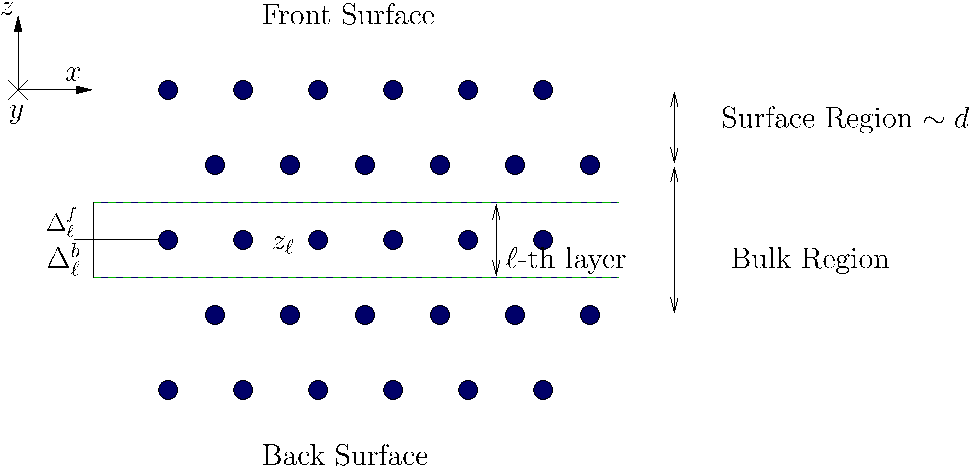
\includegraphics[height=5cm,width=7cm]{slab}
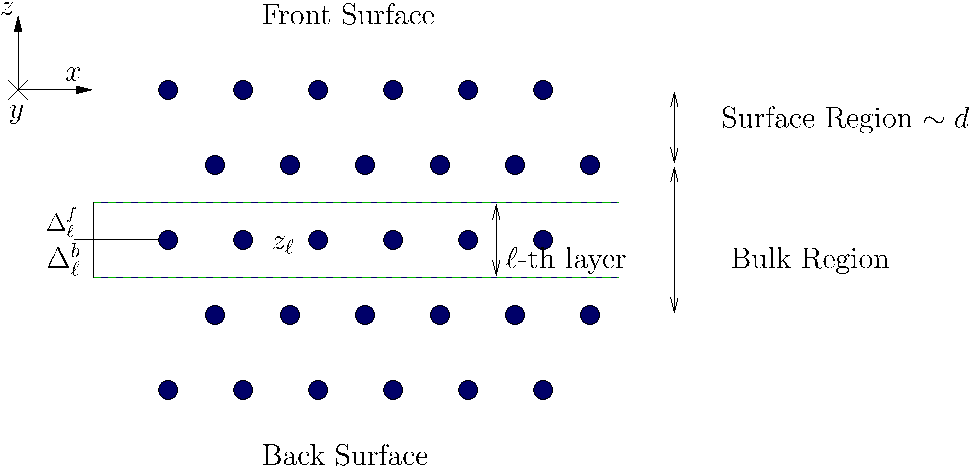
\includegraphics[scale=.7]{slab}
\caption{
We show a sketch of the slab, where the small
circles represent the atoms. See the text for the details.
}
\label{fslab}
\end{figure}

Now, we show how this ``cut function'' $S_\ell(z)$ is introduced in
the calculation of $\chi_{ijl}$.
The microscopic current density is given by
\begin{equation}\label{jmic}
\bfj(\bfr,t)=\mathrm{Tr}(\hat\bfj(\bfr)\hat\rho(t)),
\end{equation}
where the operator for the electron's current is
\begin{equation}\label{hatjmic}
\hat\bfj(\bfr)=\frac{e}{2}\left(\hat\bfv\ket{\bfr}\bra{\bfr}+\ket{\bfr}\bra{\bfr}\hat\bfv\right),
\end{equation}
where $\hat{\mbf{v}}$ is the electron's velocity operator to be dealt
with below. We define
$\hat\mu\equiv\ket{\bfr}\bra{\bfr}$ and use the cyclic invariance of
the trace to write
\begin{eqnarray}\label{jmic2}
\mathrm{Tr}(\hat\bfj(\bfr)\hat\rho(t)&=&\mathrm{Tr}(\hat\rho(t)\hat\bfj(\bfr))=
\frac{e}{2}
\left(
\mathrm{Tr}(\hat\rho\hat\bfv\hat\mu)
+
\mathrm{Tr}(\hat\rho\hat\mu\hat\bfv)
\right)
\nonumber\\
&=&
\frac{e}{2}
\sum_{n\bfk}
\left(
\bra{n\bfk}\hat\rho\hat\bfv\hat\mu\ket{n\bfk}
+
\bra{n\bfk}\hat\rho\hat\mu\hat\bfv\ket{n\bfk}
\right)
\nonumber\\
&=&
\frac{e}{2}
\sum_{nm\bfk}
\bra{n\bfk}\hat\rho\ket{m\bfk}
\left(
\bra{m\bfk}\hat\bfv\ket{\bfr}\braket{\bfr}{n\bfk}
+
\braket{m\bfk}{\bfr}\bra{\bfr}\hat\bfv\ket{n\bfk}
\right)
\nonumber\\
\bfj(\bfr,t)&=&
\sum_{nm\bfk}
\rho_{nm}(\bfk;t)\bfj_{mn}(\bfk;\bfr),
\end{eqnarray}
where
\begin{equation}\label{jmic3}
\bfj_{mn}(\bfk;\bfr)=
\frac{e}{2}
\left(
\bra{m\bfk}\hat\bfv\ket{\bfr}\braket{\bfr}{n\bfk}
+
\braket{m\bfk}{\bfr}\bra{\bfr}\hat\bfv\ket{n\bfk}
\right),
\end{equation}
are the matrix elements of the microscopic current operator,
and we have used the fact that the matrix elements between states $\ket{n\bfk}$
are diagonal in $\bfk$, i.e. proportional to $\gd(\bfk-\bfk')$.

Integrating the microscopic current $\mbf{j}(\mbf{r},t)$ over
the entire slab gives the total macroscopic current density, 
 however, if we want the
contribution from only one region of the unit cell towards the total
current, we can integrate $\mathbf{j}({\mathbf r},t)$ over the
desired region. The contribution to the current density from the
$\ell$-th layer of the slab is given by
\begin{equation}\label{jsz}
\frac{1}{\Omega}\int d^3r\, S_{\ell}(z)\, \mathbf{j}(\mathbf{r},t)
 \equiv \mathbf{J}^{(\ell)}(t),
\end{equation}
where $\mathbf{J}^{(\ell)}(t)$ is the microscopic current  in the
$\ell$-th layer.
Therefore we define
\begin{equation}\label{vcal}
e{\boldsymbol{\mathcal{V}}}^{(\ell)}_{mn}(\mathbf{k})
\equiv
%\frac{1}{\Omega}
\int d^3r\, S_{\ell}(z)\,\bfj_{mn}({\bfk};\bfr),
\end{equation}
to write
\begin{equation}\label{jmac}
J_a^{(N,\ell)}(t)=\frac{e}{\gO}
\sum_{mn\bfk}
\mathcal{V}^{a(\ell)}_{mn}(\mathbf{k})
\rho^{(N)}_{nm}(\bfk;t),
\end{equation}
as the induced macroscopic current, to order $N$-th in the external
perturbation, of the  $\ell$-th layer. The matrix elements of the
density operator for $N=1,2$ are given by Eqs.~\eqref{rho1} and
~\eqref{rho2}, respectively. 

We proceed to give an explicit expression for 
$\mathcal{V}^{a(\ell)}_{mn}(\mathbf{k})$,
for which we should work with  
the velocity operator, that is given by
\begin{eqnarray}\label{vop2} 
i\hbar\hat{\mbf{v}}&=&[\hat{\mbf{r}},\hat{H}_0]
\nonumber\\
&=&
[\hat{\mbf{r}},\frac{\hat{\mbf{p}}^2}{2m} +
\hat{V}(\mbf{r})+\hat{v}(\mbf{r},\hat{\mbf{p}})]
\approx
[\hat{\mbf{r}},\frac{\hat{\mbf{p}}^2}{2m}]=i\hbar\frac{\hat{\mbf{p}}}{m},
\end{eqnarray} 
where the possible contribution of 
the non-local pseudopotential $\hat{v}(\mbf{r},\hat{\mbf{p}})$
is neglected. Now, from above equation,
\begin{equation}\label{velo}
m\hat{\mbf{v}}\approx\hat{\mbf{p}}=-i\hbar\mbg{\nabla},
\end{equation}
is the explicit functional form of the velocity or momentum operator.
From Eq.~\eqref{jmic3}, we need 
\begin{equation}\label{vnm}
\langle \mathbf{r} | \hat{\mathbf v} | n\mathbf{k} \rangle
=\int d^3 r' \bra{\mbf{r}}\hat{\mbf{v}}\ket{\mbf{r}'}
\braket{\mbf{r}'}{n\mbf{k}}
\approx\frac{1}{m}\hat{\mbf{p}}\psi_{n\mathbf{k}}(\mathbf{r}),
\end{equation} 
where we used 
\begin{equation}\label{rvnk}
\bra{\bfr}\hat{v^x}\ket{\bfr'}
\approx \frac{1}{m}\bra{\bfr}\hat{p^x}\ket{\bfr'}
=
\gd(y-y')\gd(z-z')\left(-i\hbar\frac{\partial}{\partial x}\gd(x-x')\right),
\end{equation}
with similar results for the $y$ and $z$ Cartesian directions.
Now, from
Eqs.~\eqref{vcal} and \eqref{jmic3} we obtain
\begin{equation}
{\boldsymbol{\mathcal{V}}}^{(\ell)}_{mn}({\mathbf k})=
\frac{1}{2}
\int \mathrm{d}^3 r\,
 S_{\ell}(z)
\bigg[
\langle m\mathbf{k}|\mathbf{v} | \mathbf{r}\rangle
\langle \mathbf{r} | n \mathbf k \rangle +
\langle m\mathbf{k} | \mathbf{r}\rangle
\langle \mathbf{r} | \mathbf{v} | n \mathbf k \rangle\bigg],
\label{intj}
\end{equation}  
and using Eq.~\eqref{vnm},
we can write, for any  function $S(z)$ used
to identify the response from a region of the slab, that
\begin{eqnarray}\label{pofs}
{\boldsymbol{\mathcal{V}}}_{mn}(\mathbf{k})&\approx&
\frac{1}{2m}\int d^3 r
S(z)
 \bigg[
\psi_{n\mathbf{k}}(\mathbf{r})
\hat\bfp^*\psi^*_{m\mathbf{k}}(\mathbf{r})
+ 
\psi^*_{m\mathbf{k}}(\mathbf{r})\hat\bfp
\psi_{n\mathbf{k}}(\mathbf{r})
\bigg], \label{pofs1}  \\
&=&
\frac{1}{m}\int d^3 r
\psi^*_{m\mathbf{k}}(\mathbf{r})
\left[\frac{S(z) \mathbf{p} +
\mathbf{p} S(z)}{2}\right]
\psi_{n\mathbf{k}}(\mathbf{r})
,\label{pofs2} \\
&=&\frac{1}{m}\int d^3 r
\psi^*_{m\mathbf{k}}(\mathbf{r})\hat{\boldsymbol{\mathcal{P}}}
\psi_{n\mathbf{k}}(\mathbf{r})\equiv \frac{1}{m}{\boldsymbol{\mathcal{P}}}_{mn}(\mathbf{k}).
\end{eqnarray}
Here an integration by parts is performed on the first term of the
right hand side of Eq.~\eqref{pofs1}; since the
$\braket{\bfr}{n\bfk}=e^{-\mathrm{i}\mathbf{k}\cdot\mathbf{r}}\psi_{n\mathbf{k}}(\mathbf{r})$ 
are periodic over the unit cell, the surface term vanishes. From
Eqs.~\eqref{pofs} we see that the replacement 
\begin{equation}\label{pcali}
\hat{\mbf{p}} \to \hat{\boldsymbol{\mathcal{P}}}=\left[\frac{S(z) \hat{\mathbf{p}} +
\hat{\mathbf{p}} S(z)}{2}\right],
\end{equation}
is what it takes to change the
momentum operator of the electron, $\hat{\mbf{p}}$, to the new momentum
operator $\hat{\calbp}$ that implicitly takes into account the
contribution of the region of the slab given by $S(z)$.
Note that $\hat{\calbp}$ is properly symmetrized.

Finally, the Fourier component of macroscopic current of Eq.~\eqref{jmac} is given by
\begin{equation}\label{jmac2}
J_{\rma}^{(N,\ell)}(\go_3)=\frac{e}{m\gO}
\sum_{mn\bfk}
\calp^{\rma(\ell)}_{mn}(\mathbf{k})
\rho^{(N)}_{nm}(\bfk;\go_3),
\end{equation}
where the non-local contribution of $H_0$ is neglected, and from Eq.~\eqref{pofs2}
\begin{equation}\label{calpmn}
\calp_{mn}^{\rma(\ell)}=\int d^3 r
\psi^*_{m\mathbf{k}}(\mathbf{r})
\left[\frac{S_\ell(z) p^{\rma} +
p^{\rma} S_\ell(z)}{2}\right]
\psi_{n\mathbf{k}}(\mathbf{r}).
\end{equation}

Actually, 
to limit the response to one surface, 
the Eq.~\eqref{pcali} was proposed 
in Ref.~\onlinecite{reiningPRB94}, and latter used in Refs.
\onlinecite{mendozaPRB01} 
and \onlinecite{mejiaSMF04} in the context of SHG. Then, 
the layer-by-layer analysis of Refs. \onlinecite{hoganPRB03} 
and \onlinecite{castilloPRB03}
actually used Eq.~\eqref{sz}
thus limiting the current response
to a particular layer of the slab, and used it to obtain the
anisotropic linear optical response of semiconductor surfaces.
However, the first formal derivation of this scheme is presented in
Ref.~\onlinecite{mendozaPRB06} for the linear optical response, and
here for the non-linear optical response of semiconductors.

From the following well known result,
$im_e\go_{nm}\bfr_{nm}=\bfp_{nm}\,(n\neq m)$,
we can write
\begin{equation}\label{rcal}
{\cal R}^{\rma}_{nm}=\frac{{\cal P}^{\rma}_{nm}}{im_e\go_{nm}}\quad(n\neq m)
,
\end{equation} 

\section{Non-linear Surface Susceptibility}\label{nonchi}

In this section we obtain the expressions for the non-linear
surface susceptibility tensor to second order in the perturbing fields.
We start with the 
non-linear polarization $\mbf{P}$ written as
\begin{eqnarray}\label{mshg}
P_{\rma}(\go_3)&=&\chi_{\rma\rmb\rmc}(-\go_3;\go_1,\go_2)
E_{\rmb}(\go_1)
E_{\rmc}(\go_2)
\nonumber \\
&&+
\chi_{\rma\rmb\rmc\rml}(-\go_3;\go_1,\go_2)
E_{\rmb}(\go_1)\nabla_{\rmc} E_{\rml}(\go_2)
+\cdots,
\end{eqnarray}
where $\chi_{\rma\rmb\rmc}$ and $\chi_{\rma\rmb\rmc\rml}$,
correspond to the dipolar and quadrupolar susceptibilities,
respectively,
and the sum continues
with higher multipolar terms.
If we consider a semi-infinite system with a centrosymmetric bulk,
above equation splits, due to symmetry considerations alone, into two
contributions, one from the surface of the system and the other from
the bulk of the system. Indeed, let's take
\begin{equation}\label{mshg2}
P_{\rma}(\mbf{r})=\chi_{\rma\rmb\rmc}E_{\rmb}(\mbf{r})E_{\rmc}(\mbf{r})
+
\chi_{\rma\rmb\rmc\rml}E_{\rmb}(\mbf{r})\frac{\partial}{\partial
  \mbf{r}_{\rmc}} E_{\rml}(\mbf{r}) 
+\cdots,
\end{equation}
as the polarization with respect to the original coordinate system, and 
\begin{eqnarray}\label{mshg3}
P_{\rma}(-\mbf{r})&=&\chi_{\rma\rmb\rmc}E_{\rmb}(-\mbf{r})E_{\rmc}(-\mbf{r})
\nonumber \\
&&+
\chi_{\rma\rmb\rmc\rml}E_{\rmb}(-\mbf{r})\frac{\partial}{\partial(-
  \mbf{r}_{\rmc})} E_{\rml}(-\mbf{r}) 
+\cdots, 
\end{eqnarray}
as the polarization in the coordinate system where inversion is taken,
i.e. $\mbf{r} \to -\mbf{r}$. 
Note that we have kept the same susceptibility tensors, since as the
system is centrosymmetric, they must be invariant under $\mbf{r} \to
-\mbf{r}$. 
Recalling that $\mbf{P}(\mbf{r})$ and
$\mbf{E}(\mbf{r})$, are polar vectors,\cite{Jackson75} we have that
Eq.~\eqref{mshg3} reduces to
\begin{eqnarray}\label{mshg4}
-P_{\rma}(\mbf{r})&=&\chi_{\rma\rmb\rmc}(-E_{\rmb}(\mbf{r}))(-E_{\rmc}(\mbf{r}))
-
\chi_{\rma\rmb\rmc\rml}(-E_{\rmb}(\mbf{r}))(-\frac{\partial}{\partial\mbf{r}_{\rmc}})(-
E_{\rml}(\mbf{r})) 
+\cdots,
\nonumber \\
P_{\rma}(\mbf{r})&=&-\chi_{\rma\rmb\rmc}E_{\rmb}(\mbf{r})E_{\rmc}(\mbf{r})
+
\chi_{\rma\rmb\rmc\rml}E_{\rmb}(\mbf{r})\frac{\partial}{\partial\mbf{r}_{\rmc}}
E_{\rml}(\mbf{r}) 
+\cdots,
\end{eqnarray}
that when compared with Eq.~\eqref{mshg2}
leads to the conclusion that
\begin{equation}\label{sshg}
\chi_{\rma\rmb\rmc}=0 \quad\quad\mbox{for a centrosymmetric bulk}.
\end{equation}

\begin{figure}[t]
\centering
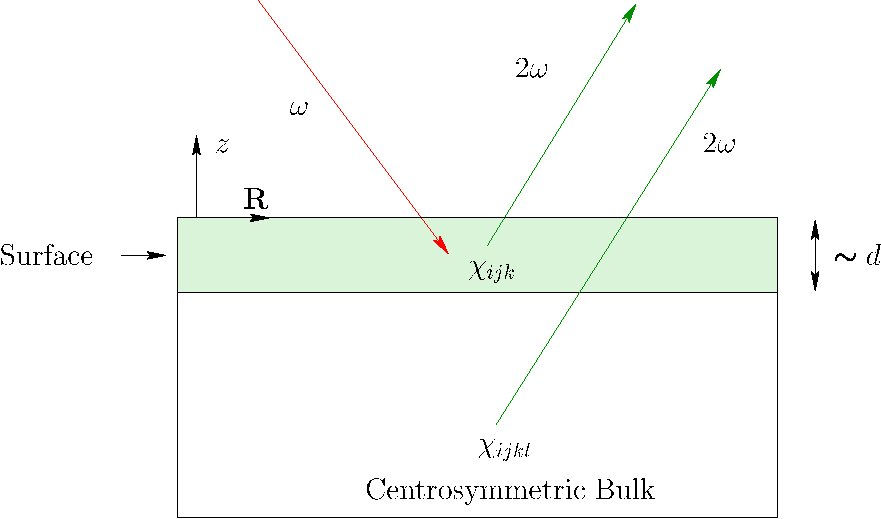
\includegraphics[scale=0.6]{system}
\caption{(color online) We show a sketch of the 
semi-infinite system with a centrosymmetric bulk. The surface region is
of width $\sim d$. The incoming photon of frequency $\go$ is represented by
a downward red arrow, whereas both the surface and bulk created second
harmonic photons of frequency $2\go$ are represented by an upward
green arrow. The red color suggests an infrared incoming photon whose
second harmonic generated photon is in the green. The dipolar,
$\chi_{\rma\rmb\rmc}$, and 
quadrupolar, $\chi_{\rma\rmb\rmc\rml}$, susceptibility tensors are shown in the regions where they
are different from zero. The axis are also shown, with $z$
perpendicular to the surface and $\mbf{R}$ parallel to it.
}
\label{fsystem}
\end{figure}

Therefore, if we move to the surface of the semi-infinite system, the
assumption of centrosymmetry necessarily breaks down, and there is no
restriction in $\chi_{\rma\rmb\rmc}$. Thus, we conclude that the leading term
of the polarization in a surface region is given by
\begin{eqnarray}\label{sshgp1}
\int d\mbf{R}\int dz 
P_{\rma}(\mbf{R},z)
&\approx&
\cals dP_{\rma}
\nonumber\\
&=&
\cals P_{\rma}^{s}
\nonumber\\
&=&
\chi_{\rma\rmb\rmc}E_{\rmb}E_{\rmc},
\end{eqnarray}
where $\mbf{R}$ is a vector parallel to the surface which is
perpendicular to $z$, $\cals$ is the surface area of the unit
cell that characterizes the surface of the system, and $d$ is the
surface region from which the dipolar signal of $\bfP$ is
different from zero (see Fig.~\ref{fsystem}).
Also, $d\mbf{P}\equiv \mbf{P}^s$ is
the surface SH polarization, given by
\begin{eqnarray}\label{sshgp2}
P_{\rma}^{s}&=&\frac{1}{\cals}
\chi_{\rma\rmb\rmc}E_{\rmb}E_{\rmc}
=
\chi^s_{\rma\rmb\rmc}E_{\rmb}E_{\rmc},
\end{eqnarray}
with $\chi_{\rma\rmb\rmc}^s=\chi_{\rma\rmb\rmc}/\cals$ the surface
non-linear susceptibility. 
On the other hand, 
\begin{equation}\label{sshgp3}
P^b_{\rma}(\mbf{r})=\chi_{\rma\rmb\rmc\rml}E_{\rmb}(\mbf{r})\nabla_{\rmc}
E_{\rml}(\mbf{r}),  
\end{equation}
gives the bulk polarization. Immediately we see that the surface
polarization is of dipolar order, whereas the bulk polarization is of
quadrupolar order, and that the rank of the susceptibility tensors is 3
for the surface, i.e. $\chi_{\rma\rmb\rmc}$, and 4 for the bulk,
i.e. $\chi_{\rma\rmb\rmc\rml}$. 
Although the bulk generated SH is in itself a very important optical
phenomena, in here we concentrate only in the surface generated
SH. Indeed, in centrosymmetric systems for which the quadrupolar bulk
response is much smaller that the dipolar surface response, SH is
readily used as a very useful and powerful optical surface probe.\cite{downer01}

To calculate $\chi_{\rma\rmb\rmc}^s$,
we start from the basic relation, $\bfJ=d\bfP/dt$ 
with $\bfJ$ the current calculated in Sec.~\ref{cd}, and
from Eq.~\eqref{jmac2} we obtain
\begin{equation}\label{Pjikn}
J_{\rma}^{(2,\ell)}(\go_3)=-i\go_3P_{\rma}(\go_3)
=\frac{e}{m_e\gO}
\sum_{mn\bfk}
\calp^{\rma(\ell)}_{mn}(\mathbf{k})
\rho^{(2)}_{nm}(\bfk;\go_3)
,
\end{equation}
which upon using Eqs.~\eqref{rho2} and ~\eqref{sshgp2} leads to
\begin{eqnarray}\label{Pjikn2}
\chi^{s(\ell)}_{\rma\rmb\rmc}(-\go_3;\go_1,\go_2)
&=&
\frac{ie}{m_e\gO E^{\rmb}_1E^{\rmc}_2\cals \go_3}
\sum_{mn\bfk}
\calp^{\rma(\ell)}_{mn}(\mathbf{k})
\rho^{(2)}_{nm}(\bfk;\go_3)
\nonumber \\
&=&
\frac{e^2}{\cals m_e\gO\hbar\go_3}
\sum_{mn\bfk}
\frac{\calp^{\rma(\ell)}_{mn}(\mathbf{k})}
{\go_{nm\bfk}-\got_3}
\bigg[
-(B_{nm}^{\rmc}(\bfk,\go_\gb))_{;k^{\rmb}}
\nonumber \\
&&
+i\sum_\ell\left(r_{n\ell}^{\rmb}B_{\ell m}^{\rmc}(\bfk,\go_\gb) -
  B_{n\ell}^{\rmc}(\bfk,\go_\gb) 
  r_{\ell m}^{\rmb}\right)
\bigg]
,
\end{eqnarray}
which gives the surface susceptibility of layer $\ell$-th.
As can be seen
from Eq. (\ref{rho2}), $\chi^{s(\ell)}_{\rma\rmb\rmc}$ can be split into
two terms, one coming from the first term and the other
from the second term of Eq . (\ref{rho2}). Then we have, after
substituting  Eq.~\eqref{rho1}, that
\begin{equation}\label{chii}
\chi_{i,\rma\rmb\rmc}^{s(\ell)}=-\frac{e^3}{m_e\gO\hbar^2\go_3}\sum_{mn\bfk}
\frac{\calp_{mn}^{\rma(\ell)}}{\go_{nm}-\go_3}
\left(\frac{f_{mn}r_{nm}^{\rmb}}{\go_{nm}-\go_\gb}\right)_{;k^{\rmc}},
\end{equation} 
and
\begin{equation}\label{chie}
\chi_{e,\rma\rmb\rmc}^{s(\ell)}=\frac{ie^3}{m_e\gO\hbar^2\go_3}\sum_{\ell mn\bfk}
\frac{\calp_{mn}^{\rma(\ell)}}{\go_{nm}-\go_3}
\left(
\frac{r_{n\ell}^{\rmc} r_{\ell m}^{\rmb} 
f_{m\ell}}{\go_{\ell m}-\go_\gb}
-\frac{r_{n\ell}^{\rmb} r_{\ell m}^{\rmc} 
f_{\ell n}}{\go_{n \ell}-\go_\gb}
\right),
\end{equation} 
where $\boldsymbol{\chi}^{s(\ell)}_i$
 is related to intraband transitions and
$\boldsymbol{\chi}^{s(\ell)}_e$
to interband transitions. 
We mention that
Eq. (\ref{chii}) and Eq. (\ref{chie}) need to be symmetrized for intrinsic
permutation symmetry, i.e.
$\chi^{\rma\rmb\rmc}(-\go_3;\go_1,\go_2)=\chi^{\rma\rmc\rmb}(-\go_3;\go_2,\go_1)$,\cite{rashkeev98}
(for SHG $\go_1=\go_2=\go$ and $\go_3=2\go$). We mention that above
equations diverge as $\go_3\to 0$. This apparent divergence is removed
in the following section.

The generalized derivative
in Eq. (\ref{chii}) is obtained from the chain rule as
\begin{equation}\label{gene}
\left(\frac{f_{mn}r_{nm}^{\rmb}}{\go_{nm}-\go_2}\right)_{;k^{\rmc}}=
\frac{f_{mn}}{\go_{nm}-\go}\left(r_{nm}^{\rmb}\right)_{;k^{\rmc}}
-\frac{f_{mn}r_{nm}^{\rmb}}{(\go_{nm}-\go)^2}\left(\go_{nm}\right)_{;k^{\rmc}},
\end{equation}
here $(\go_{nm})_{;k^a}=(\go_{n})_{;k^a}-(\go_{m})_{;k^a}$. 
In the appendices we show that
\begin{equation}\label{wk}
(\go_{nm})_{;k^{\rmc}}=\frac{p_{nn}^{\rmc}-p_{mm}^{\rmc}}{m_e}\equiv\gD_{nm}^{\rmc}
,
\end{equation}
and that
\begin{equation}\label{rgk}
(r^{\rmb}_{nm})_{;k^{\rmc}}=\frac{r_{nm}^{\rmc}\gD_{mn}^{\rmb}+r_{nm}^{\rmb}\gD_{mn}^{\rmc}}{\go_{nm}}
+\frac{i}{\go_{nm}}\sum_\ell\left(\go_{\ell m}r_{n\ell}^{\rmc}r_{\ell m}^{\rmb}
-\go_{n \ell}r_{n\ell}^{\rmb}r_{\ell m}^{\rmc}\right).
\end{equation} 
Above formulas give a complete set of relationships in order to calculate
the nonlinear susceptibility of any given layer $\ell$ as
$\boldsymbol{\chi}^{s(\ell)}=\boldsymbol{\chi}_e^{s(\ell)}+\boldsymbol{\chi}_i^{s(\ell)}$. 
Then,
we can calculate the surface
susceptibility as 
\begin{equation}\label{chiijksur}
\chi_{\rma\rmb\rmc}^s(2\go)\equiv \sum_{\ell_0}^{\ell_d}\chi_{\rma\rmb\rmc}^{(\ell)}(2\go),
\end{equation}
where $\ell_0$ represents the first  layer right at the surface, and $\ell_d$ the
layer at a distance $\sim d$ from the surface (see
Fig.~\ref{fsystem}). Of course we can use Eq.~\eqref{chiijksur} for
either the front or the back surface.
Likewise
\begin{equation}\label{chiijklf}
\chi_{\rma\rmb\rmc}^{(\ell_f)}(2\go)\equiv \sum_{\ell_d}^{\ell_f}\chi_{\rma\rmb\rmc}^{(\ell)}(2\go),
\end{equation}
is a dipolar bulk susceptibility, with the property that,
\begin{equation}\label{chiijkbul}
\chi_{\rma\rmb\rmc}^{(\ell_f)}(2\go)\stackrel{\ell_f \to \ell_b}{=} 0,
\end{equation}
where $\ell_b$ is a bulk layer such that the bulk centrosymmetry is
fully stablished and the dipolar non-linear susceptibility is
identically zero, in accordance with Eq.~\eqref{sshg}. We remark that 
$\ell_d$  is
not universal, and $\ell_b$ should be found according to Eq.~\eqref{chiijkbul}. 

\section{Divergence-free $\chi^s$}

To obtain divergence free expressions for SHG that are manageable for
programing, we take Eqs.~\eqref{chii} and \eqref{chie} and perform
a partial fraction  expansion in $\go$ to get the following terms for
the {\it intErband} term
\begin{eqnarray}\label{pfe}  
E&=&  
A
\left[
-\frac{1}{2\go_{lm}(2\go_{lm}-\go_{nm})}\frac{1}{\go_{lm}-\go}
+\frac{2}{\go_{nm}(2\go_{lm}-\go_{nm})}\frac{1}{\go_{nm}-2\go}
+\frac{1}{2\go_{lm}\go_{nm}}\frac{1}{\go}
\right]
\nonumber\\
&-& 
B
\left[
-\frac{1}{2\go_{nl}(2\go_{nl}-\go_{nm})}\frac{1}{\go_{nl}-\go}
+\frac{2}{\go_{nm}(2\go_{nl}-\go_{nm})}\frac{1}{\go_{nm}-2\go}
+\frac{1}{2\go_{nl}\go_{nm}}\frac{1}{\go}
\right]
,
\end{eqnarray}  
where 
$A=f_{ml}{\cal P}^{\rma}_{mn}r^{\rmc}_{nl}r^{\rmb}_{lm}$   
and
$B=f_{ln}{\cal P}^{\rma}_{mn}r^{\rmb}_{nl}r^{\rmc}_{lm}$,  
and the following terms for the {\it Intraband} terms
 (using Eq.~\eqref{gene})
\begin{eqnarray}\label{pfi} 
I&=& 
C
\left[
-\frac{1}{2\go^2_{nm}}\frac{1}{\go_{nm}-\go}
+\frac{2}{\go^2_{nm}}\frac{1}{\go_{nm}-2\go}
+\frac{1}{2\go^2_{nm}}\frac{1}{\go}
\right]
\nonumber\\
&-&D
\left[
-\frac{3}{2\go^3_{nm}}\frac{1}{\go_{nm}-\go}
+\frac{4}{\go^3_{nm}}\frac{1}{\go_{nm}-2\go}
+\frac{1}{2\go^3_{nm}}\frac{1}{\go}
-\frac{1}{2\go^2_{nm}}\frac{1}{(\go_{nm}-\go)^2}
\right]
,
\end{eqnarray} 
where 
$C=f_{mn}{\cal P}^{\rma}_{mn}(r^{\rmb}_{nm})_{;k^{\rmc}}$, 
and
$D=f_{mn}{\cal P}^{\rma}_{mn}r^{\rmb}_{nm}\gD^{\rmc}_{nm}$.
Time-reversal symmetry allow us to write,
$\mathbf{r}_{mn}(\mathbf{k})=\mathbf{r}_{nm}(-\mathbf{k})$,
$\mathbf{r}_{mn;\mathbf{k}}(\mathbf{k})=-\mathbf{r}_{nm;\mathbf{k}}(-\mathbf{k})$,
% along with the hermiticity condition $\mathbf{r}%
%_{mn}=\mathbf{r}_{nm}^{\ast }$, which implies that $\mathbf{r}_{mn;\mathbf{k}}=\mathbf{r}_{nm;\mathbf{k}%
%}^{\ast }$, and arrive at the following results for the imaginary parts of $
%\chi _{i,e}^{\rma\rmb\rmc}$, 
${\cal P}_{mn}^{\rma}(-\mathbf{k})=-{\cal P}_{nm}^{\rma}(\mathbf{k})$,
$\omega_{mn}^{S}(-\mathbf{k})=\omega_{mn}^{S}(\mathbf{k})$,
and
$\gD^a_{nm}(-\bfk)=-\gD^a_{nm}(\bfk)$.
Also, for a clean cold semiconductor $f_n=1$  for an occupied or
valence ($n=v$) band and $f_n=0$
for an empty or conduction ($n=c$) band independent of $\bfk$ and
$f_{nm}=-f_{mn}$. 
Then adding the $\bfk$ and $-\bfk$ terms, we
can easily show that the $1/\go$ terms in both Eq.~\eqref{pfe} and Eq.~\eqref{pfi}
cancel each other.
The last term in the second line of Eq.~\eqref{pfi} is dealt with as
follows.
\begin{eqnarray}\label{dres}
\frac{D}{2\go^2_{nm}}\frac{1}{(\go_{nm}-\go)^2}
=
\frac{f_{mn}{\cal
    P}^{\rma}_{mn}r^{\rmb}_{nm}\gD^{\rmc}_{nm}}{2\go^2_{nm}}\frac{1}{(\go_{nm}-\go)^2} 
&=&
-\frac{im_ef_{mn}}{2}
\frac{{\cal R}^{\rma}_{mn}r^{\rmb}_{nm}}{\go_{nm}}\frac{\gD^{\rmc}_{nm}}{(\go_{nm}-\go)^2}
\nonumber\\
&=&
\frac{im_ef_{mn}}{2}
\frac{{\cal R}^{\rma}_{mn}r^{\rmb}_{nm}}{\go_{nm}}
\left(
\frac{1}{\go_{nm}-\go}
\right)_{;k^{\rmc}}
\nonumber\\
&=&
-\frac{im_ef_{mn}}{2}
\left(
\frac{{\cal R}^{\rma}_{mn}r^{\rmb}_{nm}}{\go_{nm}}
\right)_{;k^{\rmc}}
\frac{1}{\go_{nm}-\go}
,
\end{eqnarray}
where we used Eqs.~\eqref{wk} and ~\eqref{rcal}, and for the last
line, we performed an
integration by parts over the Brillouin zone,
where the contribution from the edges vanishes.\cite{aschcroft}
Using the chain rule, we obtain
\begin{eqnarray}\label{chr}
\left(
\frac{{\cal R}^{\rma}_{mn}r^{\rmb}_{nm}}{\go_{nm}}
\right)_{;k^{\rmc}}
=
\frac{r^{\rmb}_{nm}}{\go_{nm}}
\left(
{\cal R}^{\rma}_{mn}
\right)_{;k^{\rmc}}
+
\frac{{\cal R}^{\rma}_{mn}}{\go_{nm}}
\left(
r^{\rmb}_{nm}
\right)_{;k^{\rmc}}
-
\frac{{\cal R}^{\rma}_{mn}r^{\rmb}_{nm}}{\go^2_{nm}}
\left(
\go_{nm}
\right)_{;k^{\rmc}}
,
\end{eqnarray}
where in the appendix \ref{calr} we 
show that (we take $\rmc\to\rmb$)
\begin{equation}\label{rgkcal}
({\cal R}^{\rma}_{nm})_{;k^{\rmb}}=\frac{
{\cal R}_{nm}^{\rma}\gD_{mn}^{\rmb}+
r_{nm}^{\rmb}\gD_{mn}^{\rma(\ell)}
}{\go_{nm}}
+\frac{i}{\go_{nm}}\sum_{\ell\ne m,n}\left(\go_{\ell m}r_{n\ell}^{\rmb}{\cal R}_{\ell m}^{\rma}
-\go_{n \ell}{\cal R}_{n\ell}^{\rma}r_{\ell m}^{\rmb}\right)
,
\end{equation}
with
\begin{equation}\label{cald}
\gD_{mn}^{\rma(\ell)}
=
{\cal V}_{mm}^{\rma(\ell)}
-
{\cal V}_{nn}^{\rma(\ell)}
=
\frac{{\cal P}_{mm}^{\rma(\ell)}
-
{\cal P}_{nn}^{\rma(\ell)}
}{m_e}
.
\end{equation}
Therefore, all the remaining non-zero terms in expressions \eqref{pfe}
and \eqref{pfi} 
are simple $\go$ and $2\go$ resonant denominators well behaved at zero
frequency. 

Using time-reversal invariance and simple index manipulation, we show
in the appendix that
\begin{equation}\label{imchiewn}
\mathrm{Im}[\chi_{e,\rma\rmb\rmc,\go}^{s(\ell)}]
=
\frac{\pi |e|^3}{2\hbar^2} 
\sum_{vc\bfk}
\sum_{l\neq(v,c)}
\left[
\frac{\go^S_{lc}\mathrm{Re}[{\cal R}^{\rma(\ell)}_{lc}\{r^{\rmb}_{cv}r^{\rmc}_{vl}\}]}
{\go^S_{cv}(2\go^S_{cv}-\go^S_{cl})}
-
\frac{\go^S_{vl}\mathrm{Re}[{\cal R}^{\rma(\ell)}_{vl}\{r^{\rmc}_{lc}r^{\rmb}_{cv}\}]}
{\go^S_{cv}(2\go^S_{cv}-\go^S_{lv})}
\right]
\gd(\go^S_{cv}-\go)
,
\end{equation}  
\begin{equation}\label{imchie2wn}
\mathrm{Im}[\chi_{e,\rma\rmb\rmc,2\go}^{s(\ell)}]
=
\frac{\pi |e|^3}{2\hbar^2} 
\sum_{vc\bfk}
4
\left[
\sum_{v'\ne v}
\frac{\mathrm{Re}[{\cal
    R}^{\rma(\ell)}_{vc}\{r^{\rmb}_{cv'}r^{\rmc}_{v'v}\}]}{2\go^S_{cv'}-\go^S_{cv}}
-
\sum_{c'\ne c}
\frac{\mathrm{Re}[{\cal R}^{\rma(\ell)}_{vc}\{r^{\rmc}_{cc'}r^{\rmb}_{c'v}\}]}
{2\go^S_{c'v}-\go^S_{cv}}
\right]
\gd(\go^S_{cv}-2\go)
,
\end{equation}
\begin{equation}\label{imchiwn}
\mathrm{Im}[\chi_{i,\rma\rmb\rmc,\go}^{s(\ell)}]
=
\frac{\pi|e|^3}{2\hbar^2}
\sum_{cv\bfk}
\frac{1}{\go^S_{cv}}
\left[
\mathrm{Im}[\{r^{\rmb}_{cv}\left({\cal R}^{\rma(\ell)}_{vc}\right)_{;k^{\rmc}}\}]
+
\frac{2\mathrm{Im}[{\cal R}^{\rma(\ell)}_{vc}\{r^{\rmb}_{cv}\gD^{\rmc}_{cv}\}]}{\go^S_{cv}}
\right]
\gd(\go^S_{cv}-\go)
,
\end{equation}
and
\begin{equation}\label{imchi2wn}
\mathrm{Im}[\chi_{i,\rma\rmb\rmc,2\go}^{s(\ell)}]
=
\frac{\pi|e|^3}{2\hbar^2}\sum_{vc\bfk}
\frac{4}{\go^S_{cv}}
\left[
\mathrm{Im}[{\cal R}^{\rma(\ell)}_{vc}\{\left(r^{\rmb}_{cv}\right)_{;k^{\rmc}}\}]
-
\frac{2\mathrm{Im}[{\cal R}^{\rma(\ell)}_{vc}\{r^{\rmb}_{cv}\gD^{\rmc}_{cv}\}]}{\go^S_{cv}}
\right]\gd(\go^S_{cv}-2\go)
,
\end{equation}
where we have split the interband and intraband $1\go$ and $2\go$
contributions. The real part of each contribution can be obtained through
a Kramers-Kronig transformation, and then
$\chi^{s(\ell)}_{\rma\rmb\rmc}=\chi^{s(\ell)}_{e,\rma\rmb\rmc,\go}+\chi^{s(\ell)}_{e,\rma\rmb\rmc,2\go}+\chi^{s(\ell)}_{i,\rma\rmb\rmc,\go}+\chi^{s(\ell)}_{i,\rma\rmb\rmc,2\go}
$. Also,
the
$\{\}$ notation symmetrizes the Cartesian indices $\rmb\rmc$, i.e. 
$\{u^{\rmb}s^{\rmc}\}=(u^{\rmb}s^{\rmc}+u^{\rmc}s^{\rmb})/2$,
from where we obtain that
$\chi_{\rma\rmb\rmc}^{s(\ell)}=\chi_{\rma\rmc\rmb}^{s(\ell)}$.
In the continuous limit of $\bfk$ 
$(1/\gO)\sum_{\bfk}\to\int d^3\bfk/(8\pi^3)$, and with the help of 
Eq.~\eqref{wk}, \eqref{rgk}, \eqref{rgkcal} and \eqref{cald}, 
Eqs.~\eqref{imchiewn}-\eqref{imchi2wn} could be
readily evaluated.

Also, since we are working in the length-gauge, it is trivial to
incorporate the scissors operator in above expressions for $\bfgchi^{s(\ell)}$
by simple taking
$\go_n\to\go_n^S$, where $\go_n^S=\go_n+(1-f_n)\Delta$ with $\gD$ the
rigid scissor correction.\cite{nastosPRB05,cabellosPRB09}

\section{Contribution of a non-local potential}
We go back to Eq.~\eqref{vop2} and keep the contribution coming form
the non-local potential, i.e.
\begin{eqnarray}\label{nl.1}
\hat{\mbf{v}}
&=&
\frac{\hat{\mbf{p}}}{m}
+
\hat\bfv^\nl
\nonumber\\
\hat\bfv^\nl
&=&
\frac{1}{i\hbar}[\hat{\mbf{r}},\hat{v}(\mbf{r},\hat{\mbf{p}})]
.
\end{eqnarray}
We get that
\begin{equation}\label{nl.2}
\langle \mathbf{r} | \hat\bfv^\nl | n\mathbf{k} \rangle
=\int d^3 r' \bra{\mbf{r}}\hat\bfv^\nl\ket{\mbf{r}'}
\braket{\mbf{r}'}{n\mbf{k}}
=\hat\bfv^\nl
\int d^3 r' \braket{\mbf{r}}{\mbf{r}'}
\braket{\mbf{r}'}{n\mbf{k}}
=\hat\bfv^\nl
\psi_{n\mathbf{k}}(\mathbf{r}),
\end{equation}
and Eq.~\eqref{intj} is now
\begin{eqnarray}\label{nl.3}
{\boldsymbol{\mathcal{V}}}^{(\ell)}_{mn}({\mathbf k})
&=&
\frac{1}{2}
\int \mathrm{d}^3 r\,
 S_{\ell}(z)
\bigg[
\langle m\mathbf{k}|\frac{\bfp}{m_e}+\bfv^\nl | \mathbf{r}\rangle
\langle \mathbf{r} | n \mathbf k \rangle +
\langle m\mathbf{k} | \mathbf{r}\rangle
\langle \mathbf{r} | \frac{\bfp}{m_e} +\bfv^\nl| n \mathbf k \rangle\bigg],
\nonumber\\
&=&
\frac{1}{2}
\int \mathrm{d}^3 r\,
 S_{\ell}(z)
\bigg[
\langle m\mathbf{k}|\frac{\bfp}{m_e}| \mathbf{r}\rangle
\langle \mathbf{r} | n \mathbf k \rangle +
\langle m\mathbf{k} | \mathbf{r}\rangle
\langle \mathbf{r} | \frac{\bfp}{m_e} | n \mathbf k \rangle\bigg],
\nonumber\\
&+&
\frac{1}{2}
\int \mathrm{d}^3 r\,
 S_{\ell}(z)
\bigg[
\langle m\mathbf{k}|\bfv^\nl | \mathbf{r}\rangle
\langle \mathbf{r} | n \mathbf k \rangle +
\langle m\mathbf{k} | \mathbf{r}\rangle
\langle \mathbf{r} | \bfv^\nl| n \mathbf k \rangle\bigg],
\nonumber\\
&=&
\frac{1}{2m_e}
\int \mathrm{d}^3 r\,
S(z)
 \bigg[
\psi_{n\mathbf{k}}(\mathbf{r})
\hat\bfp^*\psi^*_{m\mathbf{k}}(\mathbf{r})
+ 
\psi^*_{m\mathbf{k}}(\mathbf{r})\hat\bfp
\psi_{n\mathbf{k}}(\mathbf{r})
\bigg]
\nonumber\\
&+&
\frac{1}{2}
\int \mathrm{d}^3 r\,
 S_{\ell}(z)
 \bigg[
\psi_{n\mathbf{k}}(\mathbf{r})
\hat\bfv^{\nl *}\psi^*_{m\mathbf{k}}(\mathbf{r})
+ 
\psi^*_{m\mathbf{k}}(\mathbf{r})\hat\bfv^\nl
\psi_{n\mathbf{k}}(\mathbf{r})
\bigg]
\nonumber\\
&=&
\frac{1}{m_e}
\int \mathrm{d}^3 r\,
\psi^*_{m\mathbf{k}}(\mathbf{r})
\left[\frac{S(z) \mathbf{p} +
\mathbf{p} S(z)}{2}\right]
\psi_{n\mathbf{k}}(\mathbf{r})
\nonumber\\
&+&
\int \mathrm{d}^3 r\,
\psi^*_{m\mathbf{k}}(\mathbf{r})
\left[\frac{S(z) \bfv^\nl +
\bfv^\nl S(z)}{2}\right]
\psi_{n\mathbf{k}}(\mathbf{r})
\nonumber\\
&=&
\frac{1}{m_e}
\int \mathrm{d}^3 r\,
\psi^*_{m\mathbf{k}}(\mathbf{r})
\calbp^{(\ell)}
\psi_{n\mathbf{k}}(\mathbf{r})
+
\int \mathrm{d}^3 r\,
\psi^*_{m\mathbf{k}}(\mathbf{r})
\calbv^{\nl(\ell)}
\psi_{n\mathbf{k}}(\mathbf{r})
\nonumber\\
&=&
\frac{1}{m_e}
\calbp^{(\ell)}_{mn}(\bfk)
+
\calbv^{\nl(\ell)}_{mn}(\bfk)
,
\end{eqnarray}
where we used the hermitian property of $\bfp$ and $\bfv^\nl$ and  defined
\begin{eqnarray}\label{nl.4}
\calbv^{\nl(\ell)}
=
\frac{S(z) \bfv^\nl +
\bfv^\nl S(z)}{2}
,
\end{eqnarray}
and the superscript $\ell$ is inherited from $S(z)$. We would obtain,
instead of Eq.~\eqref{chii} and \eqref{chie}
\begin{equation}\label{chiinl}
\chi_{i,\rma\rmb\rmc}^{s(\ell)}=-\frac{e^3}{m_e\gO\hbar^2\go_3}\sum_{mn\bfk}
\frac{m_e{\cal V}_{mn}^{\rma(\ell)}}{\go_{nm}-\go_3}
\left(\frac{f_{mn}r_{nm}^{\rmb}}{\go_{nm}-\go_\gb}\right)_{;k^{\rmc}},
\end{equation}
and
\begin{equation}\label{chienl}
\chi_{e,\rma\rmb\rmc}^{s(\ell)}=\frac{ie^3}{m_e\gO\hbar^2\go_3}\sum_{\ell mn\bfk}
\frac{m_e{\cal V}_{mn}^{\rma(\ell)}}{\go_{nm}-\go_3}
\left(
\frac{r_{n\ell}^{\rmc} r_{\ell m}^{\rmb}
f_{m\ell}}{\go_{\ell m}-\go_\gb}
-\frac{r_{n\ell}^{\rmb} r_{\ell m}^{\rmc}
f_{\ell n}}{\go_{n \ell}-\go_\gb}
\right),
\end{equation}
where
\begin{eqnarray}\label{nl.5}
m_e{\cal V}_{mn}^{\rma(\ell)}(\bfk)=
{\cal P}^{\rma(\ell)}_{mn}(\bfk)
+
m_e{\cal V}^{\nl,\rma(\ell)}_{mn}(\bfk)
,
\end{eqnarray}

\section{Conclusions}\label{con}

We have presented a complete derivation of the required elements to
calculate the surface SHG susceptibility tensor $\bfgchi^s(2\go)$ 
using the ``layer-by-layer'' approach. We have done so for a
semiconductor using the 
length gauge for the coupling of the external electric field to the electron. 
%Also,
%we calculated the radiated efficiency $R$ within the three layer
%model. 
%The combination of $\boldsymbol{\chi}$ and $R$ allow us
%to study this fascinating surface optical phenomena.


\appendix
\section{Divergence Free Expressions for $\chi^s_{\rma\rmb\rmc}$}
We add the $\bfk$ and $-\bfk$ terms of expressions \eqref{pfe} and
\eqref{pfi} to obtain:
\begin{eqnarray}\label{chi1}
A
\left[
-\frac{1}{2\go_{lm}(2\go_{lm}-\go_{nm})}\frac{1}{\go_{lm}-\go}
\right]&=&-\frac{f_{ml}}{2}
\left[
\frac{{\cal P}^{\rma}_{mn}r^{\rmc}_{nl}r^{\rmb}_{lm}}{\go_{lm}(2\go_{lm}-\go_{nm})}\frac{1}{\go_{lm}-\go}|_{\bfk}
\right.
\nonumber\\
+
\left.
\frac{{\cal P}^{\rma}_{mn}r^{\rmc}_{nl}r^{\rmb}_{lm}}{\go_{lm}(2\go_{lm}-\go_{nm})}\frac{1}{\go_{lm}-\go}|_{-\bfk}
\right]
&=&-\frac{f_{ml}}{2}
\left[
\frac{{\cal P}^{\rma}_{mn}r^{\rmc}_{nl}r^{\rmb}_{lm}}{\go_{lm}(2\go_{lm}-\go_{nm})}\frac{1}{\go_{lm}-\go}|_{\bfk}
\right.
\nonumber\\
-
\left.
\frac{{\cal P}^{\rma}_{nm}r^{\rmc}_{ln}r^{\rmb}_{ml}}{\go_{lm}(2\go_{lm}-\go_{nm})}\frac{1}{\go_{lm}-\go}|_{\bfk}
\right]
&=&-\frac{f_{ml}}{2}
\frac{1}{\go_{lm}(2\go_{lm}-\go_{nm})}\frac{1}{\go_{lm}-\go}
\nonumber\\
&\times&
\left[
{\cal P}^{\rma}_{mn}r^{\rmc}_{nl}r^{\rmb}_{lm}
-
{\cal P}^{\rma}_{nm}r^{\rmc}_{ln}r^{\rmb}_{ml}
\right]
\\
=-\frac{f_{ml}}{2}
\frac{1}{\go_{lm}(2\go_{lm}-\go_{nm})}\frac{1}{\go_{lm}-\go}
\left[
{\cal P}^{\rma}_{mn}r^{\rmc}_{nl}r^{\rmb}_{lm}
-
({\cal P}^{\rma}_{mn}r^{\rmc}_{nl}r^{\rmb}_{lm})^*
\right]
&=&-\frac{f_{ml}}{2}
\frac{2i\mathrm{Im}[{\cal P}^{\rma}_{mn}r^{\rmc}_{nl}r^{\rmb}_{lm}]}{\go_{lm}(2\go_{lm}-\go_{nm})}\frac{1}{\go_{lm}-\go}
\nonumber
,
\end{eqnarray}
where we used the Hermiticity of the momentum and position operators.
Likewise we get that
\begin{eqnarray}\label{si}
A
\left[
\frac{2}{\go_{nm}(2\go_{lm}-\go_{nm})}\frac{1}{\go_{nm}-2\go}
\right]&=&
f_{ml}
\frac{4i\mathrm{Im}[{\cal P}^{\rma}_{mn}r^{\rmc}_{nl}r^{\rmb}_{lm}]}{\go_{nm}(2\go_{lm}-\go_{nm})}\frac{1}{\go_{nm}-2\go}
.
\end{eqnarray}
Also,
\begin{eqnarray}\label{is}
&-&
f_{ln}{\cal P}^{\rma}_{mn}r^{\rmb}_{nl}r^{\rmc}_{lm}
\left[
-\frac{1}{2\go_{nl}(2\go_{nl}-\go_{nm})}\frac{1}{\go_{nl}-\go}
+\frac{2}{\go_{nm}(2\go_{nl}-\go_{nm})}\frac{1}{\go_{nm}-2\go}
\right]
\nonumber\\
&=&
-
2if_{ln}\mathrm{Im}[{\cal P}^{\rma}_{mn}r^{\rmb}_{nl}r^{\rmc}_{lm}]
\left[
-\frac{1}{2\go_{nl}(2\go_{nl}-\go_{nm})}\frac{1}{\go_{nl}-\go}
+\frac{2}{\go_{nm}(2\go_{nl}-\go_{nm})}\frac{1}{\go_{nm}-2\go}
\right]
,
\end{eqnarray}
and therefore
\begin{eqnarray}\label{pfen}  
E&=&  
2if_{ml}\mathrm{Im}[{\cal P}^{\rma}_{mn}r^{\rmc}_{nl}r^{\rmb}_{lm}] 
\left[
-\frac{1}{2\go_{lm}(2\go_{lm}-\go_{nm})}\frac{1}{\go_{lm}-\go}
+\frac{2}{\go_{nm}(2\go_{lm}-\go_{nm})}\frac{1}{\go_{nm}-2\go}
\right]
\nonumber\\
&-& 
2if_{ln}\mathrm{Im}[{\cal P}^{\rma}_{mn}r^{\rmb}_{nl}r^{\rmc}_{lm}]
\left[
-\frac{1}{2\go_{nl}(2\go_{nl}-\go_{nm})}\frac{1}{\go_{nl}-\go}
+\frac{2}{\go_{nm}(2\go_{nl}-\go_{nm})}\frac{1}{\go_{nm}-2\go}
\right]
.
\end{eqnarray}  
Using above results into Eq.~\eqref{chie} implies
\begin{eqnarray}\label{pfen3} 
\chi_{e,\rma\rmb\rmc}^{s(\ell)}
&=& 
-\frac{2e^3}{m_e\hbar^2} 
\sum_{\ell m n\bfk}
\left[ 
f_{ml}\mathrm{Im}[{\cal P}^{\rma}_{mn}r^{\rmc}_{nl}r^{\rmb}_{lm}] 
\left[
-\frac{1}{2\go_{lm}(2\go_{lm}-\go_{nm})}\frac{1}{\go_{lm}-\go}
+\frac{2}{\go_{nm}(2\go_{lm}-\go_{nm})}\frac{1}{\go_{nm}-2\go}
\right]
\right.
\nonumber\\
&-&
\left. 
f_{ln}\mathrm{Im}[{\cal P}^{\rma}_{mn}r^{\rmb}_{nl}r^{\rmc}_{lm}]
\left[
-\frac{1}{2\go_{nl}(2\go_{nl}-\go_{nm})}\frac{1}{\go_{nl}-\go}
+\frac{2}{\go_{nm}(2\go_{nl}-\go_{nm})}\frac{1}{\go_{nm}-2\go}
\right]
\right]
\nonumber\\
&=& 
-\frac{2e^3}{m_e\hbar^2} 
\sum_{\ell m n\bfk}
\left[ 
f_{ml}\mathrm{Im}[{\cal P}^{\rma}_{mn}\{r^{\rmc}_{nl}r^{\rmb}_{lm}\}] 
\left[
-\frac{1}{2\go_{lm}(2\go_{lm}-\go_{nm})}\frac{1}{\go_{lm}-\go}
+\frac{2}{\go_{nm}(2\go_{lm}-\go_{nm})}\frac{1}{\go_{nm}-2\go}
\right]
\right.
\nonumber\\
&-&
\left. 
f_{ln}\mathrm{Im}[{\cal P}^{\rma}_{mn}\{r^{\rmb}_{nl}r^{\rmc}_{lm}\}]
\left[
-\frac{1}{2\go_{nl}(2\go_{nl}-\go_{nm})}\frac{1}{\go_{nl}-\go}
+\frac{2}{\go_{nm}(2\go_{nl}-\go_{nm})}\frac{1}{\go_{nm}-2\go}
\right]
\right]
,
\end{eqnarray}  
where $\{\}$ is the symmetrization of the Cartesian indices $\rmb\rmc$, i.e. 
$\{u^{\rmb}s^{\rmc}\}=(u^{\rmb}s^{\rmc}+u^{\rmc}s^{\rmb})/2$. 
Then, we see that
$\chi_{e,\rma\rmb\rmc}^{s(\ell)}=\chi_{e,acb}^{s(\ell)}$. We further simplify 
the last equation as follows:
\begin{eqnarray}\label{pfen2} 
\chi_{e,\rma\rmb\rmc}^{s(\ell)}
&=& 
-\frac{2e^3}{2m_e\hbar^2} 
\sum_{\ell m n\bfk}
\left[
\left[
-\frac{f_{ml}\mathrm{Im}[{\cal P}^{\rma}_{mn}\{r^{\rmc}_{nl}r^{\rmb}_{lm}\}]}
{2\go_{lm}(2\go_{lm}-\go_{nm})}\frac{1}{\go_{lm}-\go}
+\frac{2 f_{ml}\mathrm{Im}[{\cal P}^{\rma}_{mn}\{r^{\rmc}_{nl}r^{\rmb}_{lm}\}]}
{\go_{nm}(2\go_{lm}-\go_{nm})}\frac{1}{\go_{nm}-2\go}
\right]
\right.
\nonumber\\
&+&
\left.
\left[
\frac{f_{ln}\mathrm{Im}[{\cal P}^{\rma}_{mn}\{r^{\rmb}_{nl}r^{\rmc}_{lm}\}]}
{2\go_{nl}(2\go_{nl}-\go_{nm})}\frac{1}{\go_{nl}-\go}
-\frac{2 f_{ln}\mathrm{Im}[{\cal P}^{\rma}_{mn}\{r^{\rmb}_{nl}r^{\rmc}_{lm}\}]
}{\go_{nm}(2\go_{nl}-\go_{nm})}\frac{1}{\go_{nm}-2\go}
\right]
\right]
\nonumber\\
&=&
-\frac{2e^3}{m_e\hbar^2} 
\sum_{\ell m n\bfk}
\left[
\left[
\frac{2 f_{ml}\mathrm{Im}[{\cal P}^{\rma}_{mn}\{r^{\rmc}_{nl}r^{\rmb}_{lm}\}]}
{\go_{nm}(2\go_{lm}-\go_{nm})}
-\frac{2 f_{ln}\mathrm{Im}[{\cal P}^{\rma}_{mn}\{r^{\rmb}_{nl}r^{\rmc}_{lm}\}]
}{\go_{nm}(2\go_{nl}-\go_{nm})}
\right]
\frac{1}{\go_{nm}-2\go}
\right.
\nonumber\\
&+&
\left.
\left[
\frac{f_{ln}\mathrm{Im}[{\cal P}^{\rma}_{mn}\{r^{\rmb}_{nl}r^{\rmc}_{lm}\}]}
{2\go_{nl}(2\go_{nl}-\go_{nm})}\frac{1}{\go_{nl}-\go}
-\frac{f_{ml}\mathrm{Im}[{\cal P}^{\rma}_{mn}\{r^{\rmc}_{nl}r^{\rmb}_{lm}\}]}
{2\go_{lm}(2\go_{lm}-\go_{nm})}
\frac{1}{\go_{lm}-\go}|_{\ell\leftrightarrow m}
\right]
\right]
\nonumber\\
&=&
-\frac{e^3}{m_e\hbar^2} 
\sum_{\ell m n\bfk}
\left[
\left[
\frac{2 f_{ml}\mathrm{Im}[{\cal P}^{\rma}_{mn}\{r^{\rmc}_{nl}r^{\rmb}_{lm}\}]}
{\go_{nm}(2\go_{lm}-\go_{nm})}
-\frac{2 f_{ln}\mathrm{Im}[{\cal P}^{\rma}_{mn}\{r^{\rmb}_{nl}r^{\rmc}_{lm}\}]
}{\go_{nm}(2\go_{nl}-\go_{nm})}
\right]
\frac{1}{\go_{nm}-2\go}
\right.
\nonumber\\
&+&
\left.
\left[
\frac{f_{ln}\mathrm{Im}[{\cal P}^{\rma}_{mn}\{r^{\rmb}_{nl}r^{\rmc}_{lm}\}]}
{2\go_{nl}(2\go_{nl}-\go_{nm})}\frac{1}{\go_{nl}-\go}
-\frac{f_{lm}\mathrm{Im}[{\cal P}^{\rma}_{ln}\{r^{\rmc}_{nm}r^{\rmb}_{ml}\}]}
{2\go_{ml}(2\go_{ml}-\go_{nl})}\frac{1}{\go_{ml}-\go}|_{n\leftrightarrow m}
\right]
\right]
\nonumber\\
&=&
-\frac{e^3}{m_e\hbar^2} 
\sum_{\ell m n\bfk}
\left[
\left[
\frac{2 f_{ml}\mathrm{Im}[{\cal P}^{\rma}_{mn}\{r^{\rmc}_{nl}r^{\rmb}_{lm}\}]}
{\go_{nm}(2\go_{lm}-\go_{nm})}
-\frac{2 f_{ln}\mathrm{Im}[{\cal P}^{\rma}_{mn}\{r^{\rmb}_{nl}r^{\rmc}_{lm}\}]
}{\go_{nm}(2\go_{nl}-\go_{nm})}
\right]
\frac{1}{\go_{nm}-2\go}
\right.
\nonumber\\
&+&
\left.
\left[
\frac{f_{ln}\mathrm{Im}[{\cal P}^{\rma}_{mn}\{r^{\rmb}_{nl}r^{\rmc}_{lm}\}]}
{2\go_{nl}(2\go_{nl}-\go_{nm})}\frac{1}{\go_{nl}-\go}
-\frac{f_{ln}\mathrm{Im}[{\cal P}^{\rma}_{lm}\{r^{\rmc}_{mn}r^{\rmb}_{nl}\}]}
{2\go_{nl}(2\go_{nl}-\go_{ml})}\frac{1}{\go_{nl}-\go}
\right]
\right]
\nonumber\\
&=&
-\frac{e^3}{m_e\hbar^2} 
\sum_{\ell m n\bfk}
\left[
\left[
\frac{2 f_{ml}\mathrm{Im}[{\cal P}^{\rma}_{mn}\{r^{\rmc}_{nl}r^{\rmb}_{lm}\}]}
{\go_{nm}(2\go_{lm}-\go_{nm})}
-\frac{2 f_{ln}\mathrm{Im}[{\cal P}^{\rma}_{mn}\{r^{\rmb}_{nl}r^{\rmc}_{lm}\}]
}{\go_{nm}(2\go_{nl}-\go_{nm})}
\right]
\frac{1}{\go_{nm}-2\go}
\right.
\nonumber\\
&+&
\left. 
f_{ln}
\left[
\frac{\mathrm{Im}[{\cal P}^{\rma}_{mn}\{r^{\rmb}_{nl}r^{\rmc}_{lm}\}]}
{2\go_{nl}(2\go_{nl}-\go_{nm})}
-\frac{f_{ln}\mathrm{Im}[{\cal P}^{\rma}_{lm}\{r^{\rmc}_{mn}r^{\rmb}_{nl}\}]}
{2\go_{nl}(2\go_{nl}-\go_{ml})}
\right]\frac{1}{\go_{nl}-\go}
\right]
,
\end{eqnarray}  
where the 2 in the denominator of the prefactor after the first equal
sign comes from the $\bfk$ and $-\bfk$ addition, i.e. 
$\chi\to\sum_{\bfk>0}[\chi(\bfk)+\chi(-\bfk)]/2$. 
Taking $\go\to\go +i\eta$ and use
$\lim_{\eta\to 0}1/(x-i\eta)=P(1/x)+i\pi\gd(x)$, to get
\begin{eqnarray}\label{imchie}
\mathrm{Im}[\chi_{e,\rma\rmb\rmc}^{s(\ell)}]
&=&
\frac{2\pi e^3}{m_e\hbar^2} 
\sum_{\ell m n\bfk}
\left[
\left[
\frac{2 f_{ln}\mathrm{Im}[{\cal P}^{\rma}_{mn}\{r^{\rmb}_{nl}r^{\rmc}_{lm}\}]
}{\go_{nm}(2\go_{nl}-\go_{nm})}
-\frac{2 f_{ml}\mathrm{Im}[{\cal P}^{\rma}_{mn}\{r^{\rmc}_{nl}r^{\rmb}_{lm}\}]}
{\go_{nm}(2\go_{lm}-\go_{nm})}
\right]
\gd(\go_{nm}-2\go)
\right.
\nonumber\\
&+&
\left. 
f_{ln}
\left[
\frac{\mathrm{Im}[{\cal P}^{\rma}_{lm}\{r^{\rmc}_{mn}r^{\rmb}_{nl}\}]}
{2\go_{nl}(2\go_{nl}-\go_{ml})}
-
\frac{\mathrm{Im}[{\cal P}^{\rma}_{mn}\{r^{\rmb}_{nl}r^{\rmc}_{lm}\}]}
{2\go_{nl}(2\go_{nl}-\go_{nm})}
\right]
\gd(\go_{nl}-\go)
\right]
.
\end{eqnarray}  
We change $l\leftrightarrow m$ in the last term,
to write
\begin{eqnarray}\label{imchie2}
\mathrm{Im}[\chi_{e,\rma\rmb\rmc}^{s(\ell)}]
&=&
\frac{\pi e^3}{m_e\hbar^2} 
\sum_{\ell m n\bfk}
\left[
\left[
\frac{2 f_{ln}\mathrm{Im}[{\cal P}^{\rma}_{mn}\{r^{\rmb}_{nl}r^{\rmc}_{lm}\}]
}{\go_{nm}(2\go_{nl}-\go_{nm})}
-\frac{2 f_{ml}\mathrm{Im}[{\cal P}^{\rma}_{mn}\{r^{\rmc}_{nl}r^{\rmb}_{lm}\}]}
{\go_{nm}(2\go_{lm}-\go_{nm})}
\right]
\gd(\go_{nm}-2\go)
\right.
\nonumber\\
&+&
\left. 
f_{mn}
\left[
\frac{\mathrm{Im}[{\cal P}^{\rma}_{ml}\{r^{\rmc}_{ln}r^{\rmb}_{nm}\}]}
{2\go_{nm}(2\go_{nm}-\go_{lm})}
-
\frac{\mathrm{Im}[{\cal P}^{\rma}_{ln}\{r^{\rmb}_{nm}r^{\rmc}_{ml}\}]}
{2\go_{nm}(2\go_{nm}-\go_{nl})}
\right]
\gd(\go_{nm}-\go)
\right]
.
\end{eqnarray}  
From the delta functions it follows that $n=c$ and $m=v$, then
$f_{ln}=1$ with $l=v'$,
$f_{ml}=1$ with $l=c'$, 
and
$f_{mn}=1$ with $l=c'$ or $v'$, and
\begin{eqnarray}\label{imchie3}
\mathrm{Im}[\chi_{e,\rma\rmb\rmc}^{s(\ell)}]
&=&
\frac{\pi e^3}{m_e\hbar^2} 
\sum_{vc\bfk}
\left[
\left[
\sum_{v'\ne v}
\frac{2\mathrm{Im}[{\cal P}^{\rma(\ell)}_{vc}\{r^{\rmb}_{cv'}r^{\rmc}_{v'v}\}]
}{\go_{cv}(2\go_{cv'}-\go_{cv})}
-
\sum_{c'\ne c}
\frac{2\mathrm{Im}[{\cal P}^{\rma(\ell)}_{vc}\{r^{\rmc}_{cc'}r^{\rmb}_{c'v}\}]}
{\go_{cv}(2\go_{c'v}-\go_{cv})}
\right]
\gd(\go_{cv}-2\go)
\right.
\nonumber\\
&+&
\left.
\sum_{l\neq(v,c)}
\left[
\frac{\mathrm{Im}[{\cal P}^{\rma(\ell)}_{vl}\{r^{\rmc}_{lc}r^{\rmb}_{cv}\}]}
{2\go_{cv}(2\go_{cv}-\go_{lv})}
-
\frac{\mathrm{Im}[{\cal P}^{\rma(\ell)}_{lc}\{r^{\rmb}_{cv}r^{\rmc}_{vl}\}]}
{2\go_{cv}(2\go_{cv}-\go_{cl})}
\right]
\gd(\go_{cv}-\go)
\right]
,
\end{eqnarray}  
where we put the layer $\ell$ dependence in ${\cal P}$.
Using Eq.~\eqref{rcal}, we can obtain the following result
\begin{eqnarray}\label{ptor}
2i\mathrm{Im}[{\cal P}^{\rma(\ell)}_{nm}\{r^{\rmb}_{ml}r^{\rmc}_{ln}\}]
&=&
{\cal P}^{\rma(\ell)}_{nm}\{r^{\rmb}_{ml}r^{\rmc}_{ln}\}
-
({\cal P}^{\rma(\ell)}_{nm}\{r^{\rmb}_{ml}r^{\rmc}_{ln}\})^*
\nonumber\\
&=&
im_e\go_{nm}{\cal R}^{\rma(\ell)}_{nm}\{r^{\rmb}_{ml}r^{\rmc}_{ln}\}
-
(im_e\go_{nm}{\cal R}^{\rma(\ell)}_{nm}\{r^{\rmb}_{ml}r^{\rmc}_{ln}\})^*
\nonumber\\
&=&
im_e\go_{nm}\left({\cal R}^{\rma(\ell)}_{nm}\{r^{\rmb}_{ml}r^{\rmc}_{ln}\}
+
({\cal R}^{\rma(\ell)}_{nm}\{r^{\rmb}_{ml}r^{\rmc}_{ln}\})^*
\right)
\nonumber\\
&=&
2im_e\go_{nm}\mathrm{Re}[{\cal R}^{\rma(\ell)}_{nm}\{r^{\rmb}_{ml}r^{\rmc}_{ln}\}]
,
\end{eqnarray}
then, using $\go_{vc}=-\go_{vc}$ we obtain
\begin{eqnarray}\label{imchie3n}
\mathrm{Im}[\chi_{e,\rma\rmb\rmc}^{s(\ell)}]
&=&
\frac{\pi e^3}{\hbar^2} 
\sum_{vc\bfk}
\left[
\left[
-\sum_{v'\ne v}
\frac{2\mathrm{Re}[{\cal R}^{\rma(\ell)}_{vc}\{r^{\rmb}_{cv'}r^{\rmc}_{v'v}\}]
}{2\go_{cv'}-\go_{cv}}
+
\sum_{c'\ne c}
\frac{2\mathrm{Re}[{\cal R}^{\rma(\ell)}_{vc}\{r^{\rmc}_{cc'}r^{\rmb}_{c'v}\}]}
{2\go_{c'v}-\go_{cv}}
\right]
\gd(\go_{cv}-2\go)
\right.
\nonumber\\
&+&
\left.
\sum_{l\neq(v,c)}
\left[
\frac{\go_{vl}\mathrm{Re}[{\cal R}^{\rma(\ell)}_{vl}\{r^{\rmc}_{lc}r^{\rmb}_{cv}\}]}
{2\go_{cv}(2\go_{cv}-\go_{lv})}
-
\frac{\go_{lc}\mathrm{Re}[{\cal R}^{\rma(\ell)}_{lc}\{r^{\rmb}_{cv}r^{\rmc}_{vl}\}]}
{2\go_{cv}(2\go_{cv}-\go_{cl})}
\right]
\gd(\go_{cv}-\go)
\right]
.
\end{eqnarray}  
Finally, following Ref.~\onlinecite{nastosPRB05,cabellosPRB09} we simply change
$\go_{nm}\to\go_{nm}^S$ to obtain the scissored expresion of
\begin{eqnarray}\label{imchies}
\mathrm{Im}[\chi_{e,\rma\rmb\rmc}^{s(\ell)}]
&=&
\frac{\pi e^3}{2\hbar^2} 
\sum_{vc\bfk}
\left[
4
\left[
-\sum_{v'\ne v}
\frac{\mathrm{Re}[{\cal R}^{\rma(\ell)}_{vc}\{r^{\rmb}_{cv'}r^{\rmc}_{v'v}\}]
}{2\go^S_{cv'}-\go^S_{cv}}
+
\sum_{c'\ne c}
\frac{\mathrm{Re}[{\cal R}^{\rma(\ell)}_{vc}\{r^{\rmc}_{cc'}r^{\rmb}_{c'v}\}]}
{2\go^S_{c'v}-\go^S_{cv}}
\right]
\gd(\go^S_{cv}-2\go)
\right.
\nonumber\\
&+&
\left.
\sum_{l\neq(v,c)}
\left[
\frac{\go^S_{vl}\mathrm{Re}[{\cal R}^{\rma(\ell)}_{vl}\{r^{\rmc}_{lc}r^{\rmb}_{cv}\}]}
{\go^S_{cv}(2\go^S_{cv}-\go^S_{lv})}
-
\frac{\go^S_{lc}\mathrm{Re}[{\cal R}^{\rma(\ell)}_{lc}\{r^{\rmb}_{cv}r^{\rmc}_{vl}\}]}
{\go^S_{cv}(2\go^S_{cv}-\go^S_{cl})}
\right]
\gd(\go^S_{cv}-\go)
\right]
,
\end{eqnarray}  
where we have ``pulled'' a factor of 1/2, so the prefactor is the same
as that of the velocity gauge formalism.\cite{cabellosPRB09} 
For the $I$ term of Eq.~\eqref{pfi}, we notice that the energy
denominators are invariant under $\bfk\to -\bfk$, and then we only
look at the numerators, then
\begin{eqnarray}\label{ct}
C\to f_{mn}{\cal P}^{\rma}_{mn}(r^{\rmb}_{nm})_{;k^{\rmc}}|_{\bfk}
+
f_{mn}{\cal P}^{\rma}_{mn}(r^{\rmb}_{nm})_{;k^{\rmc}}|_{-\bfk}
&=&
f_{mn}\left[{\cal P}^{\rma}_{mn}(r^{\rmb}_{nm})_{;k^{\rmc}}|_{\bfk}
+
(-{\cal P}^{\rma}_{nm})(-(r^{\rmb}_{mn})_{;k^{\rmc}})|_{\bfk}
\right]
\nonumber\\
&=&
f_{mn}\left[{\cal P}^{\rma}_{mn}(r^{\rmb}_{nm})_{;k^{\rmc}}
+
{\cal P}^{\rma}_{nm}(r^{\rmb}_{mn})_{;k^{\rmc}}
\right]
\nonumber\\
&=&
f_{mn}\left[{\cal P}^{\rma}_{mn}(r^{\rmb}_{nm})_{;k^{\rmc}}
+
({\cal P}^{\rma}_{mn}(r^{\rmb}_{nm})_{;k^{\rmc}})^*
\right]
\nonumber\\
&=& 
m_ef_{mn}\go_{mn}\left[i{\cal R}^{\rma}_{mn}(r^{\rmb}_{nm})_{;k^{\rmc}}
+
(i{\cal R}^{\rma}_{mn}(r^{\rmb}_{nm})_{;k^{\rmc}})^*
\right]
\nonumber\\
&=& 
im_ef_{mn}\go_{mn}\left[{\cal R}^{\rma}_{mn}(r^{\rmb}_{nm})_{;k^{\rmc}}
-
({\cal R}^{\rma}_{mn}(r^{\rmb}_{nm})_{;k^{\rmc}})^*
\right]
\nonumber\\
&=& 
-2m_ef_{mn}\go_{mn}\mathrm{Im}[{\cal R}^{\rma}_{mn}(r^{\rmb}_{nm})_{;k^{\rmc}}]
,
\end{eqnarray}
with similar results for 
$D=-2f_{mn}\go_{mn}\mathrm{Im}[{\cal  R}^{\rma}_{mn}r^{\rmb}_{nm}]\gD^{\rmc}_{nm}$.
 Now, from Eq.~\eqref{chr}, we obtain
that the first term reduces to
\begin{eqnarray}\label{chrn}
\frac{r^{\rmb}_{nm}}{\go_{nm}}\left({\cal R}^{\rma}_{mn}\right)_{;k^{\rmc}}|_{\bfk}
+
\frac{r^{\rmb}_{nm}}{\go_{nm}}\left({\cal R}^{\rma}_{mn}\right)_{;k^{\rmc}}|_{-\bfk}
&=&
\frac{r^{\rmb}_{nm}}{\go_{nm}}\left({\cal R}^{\rma}_{mn}\right)_{;k^{\rmc}}|_{\bfk}
-
\frac{r^{\rmb}_{mn}}{\go_{nm}}\left({\cal R}^{\rma}_{nm}\right)_{;k^{\rmc}}|_{\bfk}
\nonumber\\
&=&
\frac{1}{\go_{nm}}\left[r^{\rmb}_{nm}\left({\cal R}^{\rma}_{mn}\right)_{;k^{\rmc}}
-
(r^{\rmb}_{nm}\left({\cal R}^{\rma}_{mn}\right)_{;k^{\rmc}})^*\right]
\nonumber\\
&=&
\frac{2i}{\go_{nm}}\mathrm{Im}[r^{\rmb}_{nm}\left({\cal R}^{\rma}_{mn}\right)_{;k^{\rmc}}]
,
\end{eqnarray}
with similar results for the other two terms. First, we collect the
$2\go$ terms form Eq.~\eqref{pfi} that contribute to Eq.~\eqref{chii}
\begin{eqnarray}\label{2wchii}
I_{2\go}&=&
-\frac{e^3}{2\hbar^2}\sum_{mn\bfk}
\left[
\frac{-4f_{mn}\go_{mn}\mathrm{Im}[{\cal R}^{\rma}_{mn}\left(r^{\rmb}_{nm}\right)_{;k^{\rmc}}]}{\go^2_{nm}}
-
\frac{-8f_{mn}\go_{mn}\mathrm{Im}[{\cal R}^{\rma}_{mn}r^{\rmb}_{nm}]\gD^{\rmc}_{nm}}{\go^3_{nm}}
\right]\frac{1}{\go_{nm}-2\go}
\nonumber\\
&=&
\frac{e^3}{2\hbar^2}\sum_{mn\bfk}
\left[
\frac{4f_{mn}\go_{mn}\mathrm{Im}[{\cal R}^{\rma}_{mn}\left(r^{\rmb}_{nm}\right)_{;k^{\rmc}}]}{\go^2_{nm}}
-
\frac{8f_{mn}\go_{mn}\mathrm{Im}[{\cal R}^{\rma}_{mn}r^{\rmb}_{nm}]\gD^{\rmc}_{nm}}{\go^3_{nm}}
\right]\frac{1}{\go_{nm}-2\go}
\nonumber\\
&=&
\frac{e^3}{2\hbar^2}\sum_{mn\bfk}
\left[
\frac{-4f_{mn}\mathrm{Im}[{\cal R}^{\rma}_{mn}\left(r^{\rmb}_{nm}\right)_{;k^{\rmc}}]}{\go_{nm}}
+
\frac{8f_{mn}\mathrm{Im}[{\cal R}^{\rma}_{mn}r^{\rmb}_{nm}]\gD^{\rmc}_{nm}}{\go^2_{nm}}
\right]\frac{1}{\go_{nm}-2\go}
,
\end{eqnarray}
where the 2 in the denominator of the prefactor
comes from the $\bfk$ and $-\bfk$ addition, as previously noted.
Taking $\eta\to 0$ we get that
\begin{eqnarray}\label{imchi2w}
\mathrm{Im}[\chi_{i,\rma\rmb\rmc,2\go}^{s(\ell)}]
&=&
\frac{\pi|e|^3}{2\hbar^2}\sum_{mn\bfk}
\frac{4f_{mn}}{\go_{nm}}
\left[
\mathrm{Im}[{\cal R}^{\rma}_{mn}\left(r^{\rmb}_{nm}\right)_{;k^{\rmc}}]
-
\frac{2\mathrm{Im}[{\cal R}^{\rma}_{mn}r^{\rmb}_{nm}]\gD^{\rmc}_{nm}}{\go_{nm}}
\right]\gd(\go_{nm}-2\go)
\nonumber \\
&=&
\frac{\pi|e|^3}{2\hbar^2}\sum_{vc\bfk}
\frac{4}{\go^S_{cv}}
\left[
\mathrm{Im}[{\cal R}^{\rma(\ell)}_{vc}\{\left(r^{\rmb}_{cv}\right)_{;k^{\rmc}}\}]
-
\frac{2\mathrm{Im}[{\cal R}^{\rma(\ell)}_{vc}\{r^{\rmb}_{cv}]\gD^{\rmc}_{cv}\}}{\go^S_{cv}}
\right]\gd(\go^S_{cv}-2\go)
,
\end{eqnarray} 
where from the delta term we must have $n=c$ and $m=v$. The expression
is symmetric in the last two indices and is properly scissor shifted
as well. 

The $\go$ terms are
\begin{eqnarray}\label{pfia}
I_{\go}
&=&
-\frac{e^3}{m_e2\hbar^2}
\sum_{nm\bfk}
\left[
\left[
-\frac{C}{2\go^2_{nm}}
+
\frac{3D}{2\go^3_{nm}}
\right]\frac{1}{\go_{nm}-\go}
+
\frac{D}{2\go^2_{nm}}\frac{1}{(\go_{nm}-\go)^2}
\right]
\nonumber\\
&=&
-\frac{e^3}{m_e2\hbar^2}
\sum_{nm\bfk}
\left[
\left[
-\frac{-2m_ef_{mn}\go_{mn}\mathrm{Im}[{\cal R}^{\rma}_{mn}(r^{\rmb}_{nm})_{;k^{\rmc}}]
}{2\go^2_{nm}}
+
\frac{3(-2m_ef_{mn}\go_{mn}\mathrm{Im}[{\cal R}^{\rma}_{mn}r^{\rmb}_{nm}]\gD^{\rmc}_{nm})}{2\go^3_{nm}}
\right]\frac{1}{\go_{nm}-\go}
\right.
\nonumber\\
&+&
\left.
\frac{-im_ef_{mn}}{2}
\left(
\frac{{\cal R}^{\rma}_{mn}r^{\rmb}_{nm}}{\go_{nm}}
\right)_{;k^{\rmc}}
\frac{1}{\go_{nm}-\go}
\right]
\nonumber\\
&=&
\frac{|e|^3}{2\hbar^2}
\sum_{nm\bfk}
f_{mn}
\left[
-\frac{\mathrm{Im}[{\cal R}^{\rma}_{mn}(r^{\rmb}_{nm})_{;k^{\rmc}}]
}{\go_{nm}}
+
\frac{3\mathrm{Im}[{\cal R}^{\rma}_{mn}r^{\rmb}_{nm}]\gD^{\rmc}_{nm}}{\go^2_{nm}}
-
\frac{i}{2}
\left(
\frac{{\cal R}^{\rma}_{mn}r^{\rmb}_{nm}}{\go_{nm}}
\right)_{;k^{\rmc}}
\right]\frac{1}{\go_{nm}-\go}
\nonumber\\
&=&
\frac{|e|^3}{2\hbar^2}
\sum_{nm\bfk}
f_{mn}
\left[
-\frac{\mathrm{Im}[{\cal R}^{\rma}_{mn}(r^{\rmb}_{nm})_{;k^{\rmc}}]
}{\go_{nm}}
+
\frac{3\mathrm{Im}[{\cal R}^{\rma}_{mn}r^{\rmb}_{nm}]\gD^{\rmc}_{nm}}{\go^2_{nm}}
-
\frac{i}{2}
\left[
\frac{r^{\rmb}_{nm}}{\go_{nm}}
\left(
{\cal R}^{\rma}_{mn}
\right)_{;k^{\rmc}}
\right.
\right.
\nonumber\\
&+&
\left.
\left.
\frac{{\cal R}^{\rma}_{mn}}{\go_{nm}}
\left(
r^{\rmb}_{nm}
\right)_{;k^{\rmc}}
-
\frac{{\cal R}^{\rma}_{mn}r^{\rmb}_{nm}}{\go^2_{nm}}
\left(
\go_{nm}
\right)_{;k^{\rmc}}
\right]
\right]
\frac{1}{\go_{nm}-\go}
\nonumber\\
&=&
\frac{|e|^3}{2\hbar^2}
\sum_{nm\bfk}
f_{mn}
\left[
-\frac{\mathrm{Im}[{\cal R}^{\rma}_{mn}(r^{\rmb}_{nm})_{;k^{\rmc}}]
}{\go_{nm}}
+
\frac{3\mathrm{Im}[{\cal R}^{\rma}_{mn}r^{\rmb}_{nm}]\gD^{\rmc}_{nm}}{\go^2_{nm}}
-
\frac{i}{2}
\left[
\frac{2i}{\go_{nm}}
\mathrm{Im}[r^{\rmb}_{nm}\left({\cal R}^{\rma}_{mn}\right)_{;k^{\rmc}}]
\right.
\right.
\nonumber\\
&+&
\left.
\left.
\frac{2i}{\go_{nm}}
\mathrm{Im}[
{\cal R}^{\rma}_{mn}
\left(
r^{\rmb}_{nm}
\right)_{;k^{\rmc}}
]
-
\frac{2i}{\go^2_{nm}}
\mathrm{Im}[{\cal R}^{\rma}_{mn}r^{\rmb}_{nm}]
\gD^{\rmc}_{nm}
\right]
\right]
\frac{1}{\go_{nm}-\go}
\nonumber\\
&=&
\frac{|e|^3}{2\hbar^2}
\sum_{nm\bfk}
f_{mn}
\left[
-\frac{\mathrm{Im}[{\cal R}^{\rma}_{mn}(r^{\rmb}_{nm})_{;k^{\rmc}}]
}{\go_{nm}}
+
\frac{3\mathrm{Im}[{\cal R}^{\rma}_{mn}r^{\rmb}_{nm}]\gD^{\rmc}_{nm}}{\go^2_{nm}}
+
\frac{1}{\go_{nm}}
\mathrm{Im}[r^{\rmb}_{nm}\left({\cal R}^{\rma}_{mn}\right)_{;k^{\rmc}}]
\right.
\nonumber\\
&+&
\left.
\frac{1}{\go_{nm}}
\mathrm{Im}[
{\cal R}^{\rma}_{mn}
\left(
r^{\rmb}_{nm}
\right)_{;k^{\rmc}}
]
-
\frac{1}{\go^2_{nm}}
\mathrm{Im}[{\cal R}^{\rma}_{mn}r^{\rmb}_{nm}]
\gD^{\rmc}_{nm}
\right]
\frac{1}{\go_{nm}-\go}
,
\end{eqnarray}
or
\begin{eqnarray}\label{pfian}
I_{\go}
&=&
\frac{|e|^3}{2\hbar^2}
\sum_{nm\bfk}
\frac{f_{mn}}{\go_{nm}}
\left[
-\mathrm{Im}[{\cal R}^{\rma}_{mn}(r^{\rmb}_{nm})_{;k^{\rmc}}]
+
\frac{3\mathrm{Im}[{\cal R}^{\rma}_{mn}r^{\rmb}_{nm}]\gD^{\rmc}_{nm}}{\go_{nm}}
+
\mathrm{Im}[r^{\rmb}_{nm}\left({\cal R}^{\rma}_{mn}\right)_{;k^{\rmc}}]
\right.
\nonumber\\
&+&
\left.
\mathrm{Im}[
{\cal R}^{\rma}_{mn}
\left(
r^{\rmb}_{nm}
\right)_{;k^{\rmc}}
]
-
\frac{1}{\go_{nm}}
\mathrm{Im}[{\cal R}^{\rma}_{mn}r^{\rmb}_{nm}]
\gD^{\rmc}_{nm}
\right]
\frac{1}{\go_{nm}-\go}
\nonumber\\
&=&
\frac{|e|^3}{2\hbar^2}
\sum_{nm\bfk}
\frac{f_{mn}}{\go_{nm}}
\left[
\frac{2\mathrm{Im}[{\cal R}^{\rma}_{mn}r^{\rmb}_{nm}]\gD^{\rmc}_{nm}}{\go_{nm}}
+
\mathrm{Im}[r^{\rmb}_{nm}\left({\cal R}^{\rma}_{mn}\right)_{;k^{\rmc}}]
\right]
\frac{1}{\go_{nm}-\go}
.
\end{eqnarray}
Taking $\eta\to 0$ we get that
\begin{eqnarray}\label{imchiw}
\mathrm{Im}[\chi_{i,\rma\rmb\rmc,\go}^{s(\ell)}]
&=&
\frac{\pi|e|^3}{2\hbar^2}
\sum_{cv\bfk}
\frac{1}{\go^S_{cv}}
\left[
\mathrm{Im}[\{r^{\rmb}_{cv}\left({\cal R}^{\rma(\ell)}_{vc}\right)_{;k^{\rmc}}\}]
+
\frac{2\mathrm{Im}[{\cal R}^{\rma(\ell)}_{vc}\{r^{\rmb}_{cv}]\gD^{\rmc}_{cv}\}}{\go^S_{cv}}
\right]
\gd(\go^S_{cv}-\go)
,
\end{eqnarray} 
where from the delta term we must have $n=c$ and $m=v$. The expression
is symmetric in the last two indices and is properly scissor shifted
as well. Eq.~\eqref{imchies}, \eqref{imchi2w} and \eqref{imchiw}
are the main results of this appendix, from which we have that
$\chi_{\rma\rmb\rmc}^{s(\ell)}=\chi_{e,\rma\rmb\rmc}^{s(\ell)}+\chi_{i,\rma\rmb\rmc}^{s(\ell)}$ 
where
$\chi_{i,\rma\rmb\rmc}^{s(\ell)}=\chi_{i,\rma\rmb\rmc,\go}^{s(\ell)}+\chi_{i,\rma\rmb\rmc,2\go}^{s(\ell)}$. 
In the continuous limit of $\bfk$ 
$(1/\gO)\sum_{\bfk}\to\int d^3\bfk/(8\pi^3)$ and the real part is 
obtained with a Kramers-Kronig transformation. 
We have checked that these results are equivalent to Eqs. 40 and 41 of
Cabellos et. al., Ref. \onlinecite{cabellosPRB09}, for a bulk system for which we
simply take ${\cal R}^{\rma(\ell)}_{nm}\to r^{\rma}_{nm}$.

In summary we have
\begin{eqnarray}\label{imchiew}
\mathrm{Im}[\chi_{e,\rma\rmb\rmc,\go}^{s(\ell)}]
&=&
\frac{\pi |e|^3}{2\hbar^2} 
\sum_{vc\bfk}
\sum_{l\neq(v,c)}
\left[
\frac{\go^S_{lc}\mathrm{Re}[{\cal R}^{\rma(\ell)}_{lc}\{r^{\rmb}_{cv}r^{\rmc}_{vl}\}]}
{\go^S_{cv}(2\go^S_{cv}-\go^S_{cl})}
-
\frac{\go^S_{vl}\mathrm{Re}[{\cal R}^{\rma(\ell)}_{vl}\{r^{\rmc}_{lc}r^{\rmb}_{cv}\}]}
{\go^S_{cv}(2\go^S_{cv}-\go^S_{lv})}
\right]
\gd(\go^S_{cv}-\go)
,
\end{eqnarray}  
\begin{eqnarray}\label{imchie2w}
\mathrm{Im}[\chi_{e,\rma\rmb\rmc,2\go}^{s(\ell)}]
&=&
\frac{\pi |e|^3}{2\hbar^2} 
\sum_{vc\bfk}
4
\left[
\sum_{v'\ne v}
\frac{\mathrm{Re}[{\cal
    R}^{\rma(\ell)}_{vc}\{r^{\rmb}_{cv'}r^{\rmc}_{v'v}\}]}{2\go^S_{cv'}-\go^S_{cv}}
-
\sum_{c'\ne c}
\frac{\mathrm{Re}[{\cal R}^{\rma(\ell)}_{vc}\{r^{\rmc}_{cc'}r^{\rmb}_{c'v}\}]}
{2\go^S_{c'v}-\go^S_{cv}}
\right]
\gd(\go^S_{cv}-2\go)
,
\end{eqnarray}  
\begin{eqnarray}\label{imchiwf}
\mathrm{Im}[\chi_{i,\rma\rmb\rmc,\go}^{s(\ell)}]
&=&
\frac{\pi|e|^3}{2\hbar^2}
\sum_{cv\bfk}
\frac{1}{\go^S_{cv}}
\left[
\mathrm{Im}[\{r^{\rmb}_{cv}\left({\cal R}^{\rma(\ell)}_{vc}\right)_{;k^{\rmc}}\}]
+
\frac{2\mathrm{Im}[{\cal R}^{\rma(\ell)}_{vc}\{r^{\rmb}_{cv}\gD^{\rmc}_{cv}\}]}{\go^S_{cv}}
\right]
\gd(\go^S_{cv}-\go)
,
\end{eqnarray}
and
\begin{eqnarray}\label{imchi2wf}
\mathrm{Im}[\chi_{i,\rma\rmb\rmc,2\go}^{s(\ell)}]
&=&
\frac{\pi|e|^3}{2\hbar^2}\sum_{vc\bfk}
\frac{4}{\go^S_{cv}}
\left[
\mathrm{Im}[{\cal R}^{\rma(\ell)}_{vc}\{\left(r^{\rmb}_{cv}\right)_{;k^{\rmc}}\}]
-
\frac{2\mathrm{Im}[{\cal R}^{\rma(\ell)}_{vc}\{r^{\rmb}_{cv}\gD^{\rmc}_{cv}\}]}{\go^S_{cv}}
\right]\gd(\go^S_{cv}-2\go)
,
\end{eqnarray}
where $e^3=-|e|^3$.
With the help of 
Eq.~\eqref{wk}, \eqref{rgk}, \eqref{rgkcal} and \eqref{cald} could be
readily evaluated.
\section{Some results of Dirac's notation}\label{ap_dirac}

We derive a series of results that follow from Dirac's notation and
that are  useful in the various derivations.

Let's start with the Fourier transform of the wave function written in
the \sch~ representation, i.e.
\begin{equation}\label{ap_ft}
\psi(\bfr) = \frac{1}{(2\pi\hbar)^{3/2}}\int d\bfp \psi(\bfp)e^{i\bfp\cdot\bfr/\hbar}
,
\end{equation}  
and inversely 
\begin{equation}\label{ap_tf}
\psi(\bfp) = \frac{1}{(2\pi\hbar)^{3/2}}\int d\bfr \psi(\bfr)
e^{-i\bfp\cdot\bfr/\hbar}
.
\end{equation}  
Now,
\begin{equation}\label{rpsi}
\braket{\bfr}{\psi}=\psi(\bfr)=\int d\bfp \braket{\bfr}{\bfp}\braket{\bfp}{\psi}=
\int d\bfp \braket{\bfr}{\bfp}\psi(\bfp)
,
\end{equation}
that when compared with Eq.~\eqref{ap_ft} allow us to identify,
\begin{equation}\label{rp2}
\braket{\bfr}{\bfp}=\frac{1}{(2\pi\hbar)^{3/2}}e^{i\bfp\cdot\bfr/\hbar}
.
\end{equation}
By the same token,
\begin{equation}\label{rpsi2}
\braket{\bfp}{\psi}=\psi(\bfp)=\int d\bfr \braket{\bfp}{\bfr}\braket{\bfr}{\psi}=
\int d\bfr \braket{\bfp}{\bfr}\psi(\bfr)
,
\end{equation}
that when compared with Eq.~\eqref{ap_tf} allow us to identify,
\begin{equation}\label{rp}
\braket{\bfp}{\bfr}=\frac{1}{(2\pi\hbar)^{3/2}}e^{-i\bfp\cdot\bfr/\hbar}
,
\end{equation}
where
\begin{equation}\label{ap_good}
\braket{\bfr}{\bfp}=(\braket{\bfp}{\bfr})^*
,
\end{equation}
is succinctly verified.
 
We calculate the matrix elements of $\bfp$ in the $\bfr$
representation,
\begin{eqnarray}\label{ap_matp}
\bra{\bfr}\hat{p}_x\ket{\bfr'}&=&
\int d\bfp
\bra{\bfr}\hat{p}_x\ket{\bfp}\braket{\bfp}{\bfr'} \\ \nonumber
&=&
\int d\bfp
p_x\braket{\bfr}{\bfp}\braket{\bfp}{\bfr'} \\ \nonumber
&=&
\frac{1}{(2\pi\hbar)^3}
\int d\bfp
p_x
e^{i\bfp\cdot(\bfr-\bfr')/\hbar}
\\ \nonumber
&=&
\frac{1}{(2\pi\hbar)^3}
\int dp_x
p_x
e^{ip_x(x-x')/\hbar}
\int dp_y
e^{ip_y(y-y')/\hbar}
\int dp_z
e^{ip_z(z-z')/\hbar}
\\ \nonumber
&=&
\frac{1}{2\pi\hbar}
\int dp_x
p_x
e^{ip_x(x-x')/\hbar}
\gd(y-y')
\gd(z-z')
,
\end{eqnarray}
where we used the fact that
\begin{equation}\label{ap_otra}
\hat\bfp\ket{\bfp}=\bfp\ket{\bfp}
,
\end{equation}
and that
\begin{equation}\label{ap_delta}
\gd(q-q')=\frac{1}{2\pi\hbar}
\int dp
e^{ip(q-q')/\hbar}
.
\end{equation}
Now,
\begin{equation}\label{ap_mas}
\frac{1}{2\pi\hbar}
\int dp_x
p_x
e^{ip_x(x-x')/\hbar}
=
-i\hbar\frac{\partial}{\partial x}
\int
\frac{dp_x}{2\pi\hbar}
e^{ip_x(x-x')/\hbar}
=-i\hbar\frac{\partial}{\partial x}\gd(x-x')
,
\end{equation}
from where we finally get 
\begin{equation}\label{ap_fin}
\bra{\bfr}\hat{p}_x\ket{\bfr'}=
(-i\hbar\frac{\partial}{\partial x}\gd(x-x'))
\gd(y-y')
\gd(z-z')
,
\end{equation}
with similar results for $\hat{p}_y$ and $\hat{p}_z$.
Now we can calculate
\begin{eqnarray}\label{ap_psi}
\bra{\bfr}\hat{p}_x\ket{\psi}&=&
\int d\bfr' \bra{\bfr}\hat{p}_x\ket{\bfr'}\braket{\bfr'}{\psi}
\\ \nonumber
&=&
\int dx' (-i\hbar\frac{\partial}{\partial x}\gd(x-x'))
\int dy' \gd(y-y')
\int dz' \gd(z-z')
\psi(x',y',z')
\\ \nonumber
&=&
-i\hbar
\int dx' (\frac{\partial}{\partial x}\gd(x-x'))
\psi(x',y,z)
=
-i\hbar
\frac{\partial}{\partial x}
\int dx' 
\gd(x-x')
\psi(x',y,z)
\\ \nonumber
&=&
-i\hbar
\frac{\partial}{\partial x}
\psi(x,y,z)
,
\end{eqnarray}
which confirms that in the $\bfr$ representation,
the $\hat\bfp$ operator is replaced with the differential operator
$-i\hbar\bfgnabla$. 

\section{Basic relationships}\label{ap_basic}

We present some basic results needed in the derivation of the main
results. 
 The normalization of the
states $\psi_{n\mathbf{q}}(\mathbf{r})$ are chosen such that
\begin{equation}\label{a_uno}
\psi_{m\mathbf{q}}(\mathbf{r})=\left(\frac{\Omega}{8\pi^{3}}\right)^{\frac{1}{2}}u_{m\mathbf{q}}(\mathbf{r})e^{i\mathbf{q}\cdot\mathbf{r}}
,
\end{equation}
and
\begin{equation}\label{a_dos}
\int_{\Omega}d^{3}r\,
u_{n\mathbf{k}}^{*}(\mathbf{r})u_{m\mathbf{q}}(\mathbf{r})=\delta_{nm}\delta_{\mathbf{\mathbf{k},q}}
,
\end{equation}
where $\Omega$ is the volume is the unit cell and $\gd_{a,b}$ is the
Kronecker delta that gives one if $a=b$ and zero otherwise.
For box normalization,
where we have $N$ unit cells in some volume $V=N\gO$, this gives
\begin{equation}\label{a_tres}
\int_{V}d^{3}r\,\psi_{n\mathbf{k}}^{*}(\mathbf{r})\psi_{m\mathbf{q}}(\mathbf{r})=\frac{V}{8\pi^{3}}\delta_{nm}\delta_{\mathbf{\mathbf{k},q}},
\end{equation}
which lets us have in the limit of $N\rightarrow\infty$
\begin{equation}\label{a_4}
\int
d^{3}r\,\psi_{n\mathbf{k}}^{*}(\mathbf{r})\psi_{m\mathbf{q}}(\mathbf{r})
=\delta_{nm}\delta(\mathbf{k}-\mathbf{q})
,
\end{equation}
for which the Kornecker-$\gd$ is replaced by
\begin{equation}\label{a_5}
\gd_{\bfk,\bfq}\rightarrow\frac{8\pi^3}{V}\gd(\bfk-\bfq)
,
\end{equation}
and we recall that $\gd(x)=\gd(-x)$. Now, for any periodic function
$f(\bfr)=f(\bfr+\bfR)$ we have
\begin{eqnarray}\label{a_6}
\int d^{3}r\, e^{i(\mathbf{q}-\mathbf{k})\cdot\mathbf{r}}f(\mathbf{r})
& = &
\sum_{j}^{\mbox{unit cells}}\int_{\Omega}d^{3}r\,
e^{i(\mathbf{q}-\mathbf{k})\cdot(\mathbf{r}+\mathbf{R}_{j})}f(\mathbf{r}+\mathbf{R}_{j}),
\nonumber
\\
 & =&\sum_{j}^{\mbox{unit cells}}\int_{\Omega}d^{3}r\,
 e^{i(\mathbf{q}-\mathbf{k})\cdot(\mathbf{r}+\mathbf{R}_{j})}f(\mathbf{r}),
\nonumber
\\
 & =&\int_{\Omega}d^{3}r\, e^{i(\mathbf{q}-\mathbf{k})\cdot\mathbf{r}}f(\mathbf{r})\sum_{j}^{\mbox{unit cells}}e^{i(\mathbf{q}-\mathbf{k})\cdot\mathbf{R}_{j}},\nonumber
\\
 & =&\int_{\Omega}d^{3}r\, e^{i(\mathbf{q}-\mathbf{k})\cdot\mathbf{r}}f(\mathbf{r})N\sum_{\mathbf{K}}\delta_{\mathbf{K},\mathbf{q}-\mathbf{k}},\nonumber
\\
 & =&N\int_{\Omega}d^{3}r\, e^{i(\mathbf{q}-\mathbf{k})\cdot\mathbf{r}}f(\mathbf{r})\delta_{\mathbf{0},\mathbf{q}-\mathbf{k}},\nonumber
\\
 & =&N\delta_{\mathbf{q},\mathbf{k}}\int_{\Omega}d^{3}r\, f(\mathbf{r}),\nonumber
\\
 &
 =&\frac{8\pi^{3}}{\Omega}\delta(\mathbf{q}-\mathbf{k})\int_{\Omega}d^{3}r\,
 f(\mathbf{r})
,
\end{eqnarray}
where we have assumed that $\bfk$ and $\bfq$ are restricted to the
first Brillouin zone, and thus the reciprocal lattice vector $\bfK=0$.

\section{Generalized derivative $(\go_n(\bfk))_{;\bfk}$}\label{ap_gendevomega}

We obtain the
generalized derivative $(\go_n(\bfk))_{;\bfk}$.
We start from
\begin{equation}\label{a_conH0}
\bra{n\bfk}\hat{H}_0\ket{m\bfk'}=\gd_{nm}\gd(\bfk-\bfk')\hbar\go_m(\bfk)
,
\end{equation}
then Eq.~\eqref{gendev} gives
\begin{eqnarray}\label{a_genderH0}
(H_{0,nm})_{;\bfk}&=&
\nabla_\bfk
H_{0,n m}(\bfk)
-
i
H_{0,nm}(\bfk)
\left(
\bfgxi_{nn}(\bfk)
-
\bfgxi_{mm}(\bfk)
\right)
\nonumber\\
&=&\gd_{nm}\hbar\nabla_\bfk\go_m(\bfk)
,
\end{eqnarray}
where from Eq.~\eqref{conmri3}, 
\begin{eqnarray}\label{a_rih0}
\bra{n\bfk}[\hat\bfr_i,\hat{H}_0]\ket{m\bfk}&=&
i\gd_{nm}\hbar(\go_m(\bfk))_{;\bfk}
=
i\gd_{nm}\hbar\nabla_\bfk\go_m(\bfk)
,
\end{eqnarray}
then
\begin{equation}\label{a_wgendev}
(\go_n(\bfk))_{;\bfk}=
\nabla_\bfk\go_n(\bfk)
.
\end{equation}

Now, from Eq.~\eqref{conhrnm} 
\begin{equation}\label{a_hre}
\bra{n\bfk}[\hat\bfr_e,\hat{H}_0]\ket{m\bfk}=
i\hbar\frac{\bfp_{nm}(\bfk)}{m}
\quad\quad n\ne m 
,
\end{equation}
and from Eq.~\eqref{conhr} 
\begin{equation}\label{a_hr}
\bra{n\bfk}[\hat\bfr,\hat{H}_0]\ket{m\bfk}=
i\hbar\frac{\bfp_{nm}(\bfk)}{m}
,
\end{equation}
therefore, substituting above into

\begin{equation}\label{a_hrt}
\bra{n\bfk}[\hat\bfr,\hat{H}_0]\ket{m\bfk}=
\bra{n\bfk}[\hat\bfr_i,\hat{H}_0]\ket{m\bfk}+
\bra{n\bfk}[\hat\bfr_e,\hat{H}_0]\ket{m\bfk}
,
\end{equation}
we get
\begin{equation}\label{a_hrt2}
i\hbar\frac{\bfp_{nm}(\bfk)}{m}=
i\gd_{nm}\hbar\nabla_\bfk\go_m(\bfk)
+
i\hbar(1-\gd_{nm})\frac{\bfp_{nm}(\bfk)}{m}
,
\end{equation}
from where
\begin{equation}\label{a_gradw}
\frac{\bfp_{nn}(\bfk)}{m}=
\nabla_\bfk\go_n(\bfk)
,
\end{equation}
so from Eq.~\eqref{a_wgendev}
\begin{equation}\label{a_gradw2}
(\go_n(\bfk))_{;k^{\rma}}=
\frac{p^{\rma}_{nn}(\bfk)}{m}
.
\end{equation}

\section{Generalized derivative $(\bfr_{nm}(\bfk))_{;\bfk}$}\label{ap_genderr}

We obtain the generalized derivative $(\bfr_{nm}(\bfk))_{;\bfk}$.
We start with the basic result
\begin{equation}\label{a_hrdab}
[r^{\rma},p^{\rmb}]=i\hbar\gd_{ab}
,
\end{equation}
then
\begin{equation}\label{a_hrdab2}
\bra{n\bfk}[r^{\rma},p^{\rmb}]\ket{m\bfk'}=i\hbar\gd_{ab}\gd_{nm}\gd(\bfk-\bfk')
,
\end{equation}
so
\begin{equation}\label{a_hrdab3}
\bra{n\bfk}[r^{\rma}_i,p^{\rmb}]\ket{m\bfk'}
+
\bra{n\bfk}[r^{\rma}_e,p^{\rmb}]\ket{m\bfk'}
=i\hbar\gd_{ab}\gd_{nm}\gd(\bfk-\bfk')
.
\end{equation}
From Eq.~\eqref{conmri3} and ~\eqref{gendev}
\begin{equation}\label{a_rip}
\bra{n\bfk}[r^{\rma}_i,p^{\rmb}]\ket{m\bfk'}
=i\gd(\bfk-\bfk')(p^{\rmb}_{nm})_{;k^{\rma}}
\end{equation}
\begin{equation}\label{a_ripn}
(p^{\rmb}_{nm})_{;k^{\rma}}=
\nabla_{k^{\rma}}
p^{\rmb}_{n m}(\bfk)
-
i
p^{\rmb}_{nm}(\bfk)
\left(
\xi^{\rma}_{nn}(\bfk)
-
\xi^{\rma}_{mm}(\bfk)
\right)
,
\end{equation}
and
\begin{eqnarray}\label{a_rep}
\bra{n\bfk}[r^{\rma}_e,p^{\rmb}]\ket{m\bfk'}&=&
\sum_{\ell\bfk''}
\bigg(
\bra{n\bfk}r^{\rma}_e\ket{\ell\bfk''}\bra{\ell\bfk''}p^{\rmb}\ket{m\bfk'}
\nonumber \\
&&
-
\bra{n\bfk}p^{\rmb}\ket{\ell\bfk''}\bra{\ell\bfk''}r^{\rma}_e\ket{m\bfk'}
\bigg)
\nonumber \\
&=&
\sum_{\ell\bfk''}
\bigg(
(1-\gd_{n\ell})\gd(\bfk-\bfk'')\xi^{\rma}_{n\ell}
\gd(\bfk''-\bfk')p^{\rmb}_{\ell m}
\nonumber \\
&&-
\gd(\bfk-\bfk'')p^{\rmb}_{n\ell}
(1-\gd_{\ell m})\gd(\bfk''-\bfk')\xi^{\rma}_{\ell m}
\bigg)
\nonumber \\
&=&
\gd(\bfk-\bfk')
\sum_{\ell}
\bigg(
(1-\gd_{n\ell})
\xi^{\rma}_{n\ell}
p^{\rmb}_{\ell m}
\nonumber \\
&&-
(1-\gd_{\ell m})
p^{\rmb}_{n\ell}
\xi^{\rma}_{\ell m}
\bigg)
\nonumber \\
&=&
\gd(\bfk-\bfk')
\bigg(
\sum_{\ell}
\bigg(
\xi^{\rma}_{n\ell}
p^{\rmb}_{\ell m}
-
p^{\rmb}_{n\ell}
\xi^{\rma}_{\ell m}
\bigg)
\nonumber \\
&&+
p^{\rmb}_{nm}(\xi^{\rma}_{mm}
-
\xi^{\rma}_{nn}
)
\bigg)
.
\end{eqnarray}
Using Eqs.~\eqref{a_rip} and ~\eqref{a_rep}
into Eq.~\eqref{a_hrdab3} gives
\begin{eqnarray}\label{a_rapb}
i\gd(\bfk-\bfk')
\bigg(
(p^{\rmb}_{nm})_{;k^{\rma}}
&&
-i
\sum_{\ell}
\bigg(
\xi^{\rma}_{n\ell}
p^{\rmb}_{\ell m}
-
p^{\rmb}_{n\ell}
\xi^{\rma}_{\ell m}
\bigg)
\nonumber \\
&&
-i
p^{\rmb}_{nm}(\xi^{\rma}_{mm}
-
\xi^{\rma}_{nn}
)
\bigg)
=
i\hbar\gd_{ab}\gd_{nm}\gd(\bfk-\bfk')
,
\end{eqnarray}
then
\begin{eqnarray}\label{a_rapb2}
(p^{\rmb}_{nm})_{;k^{\rma}}&=&
\hbar\gd_{ab}\gd_{nm}
+i
\sum_{\ell}
\bigg(
\xi^{\rma}_{n\ell}
p^{\rmb}_{\ell m}
-
p^{\rmb}_{n\ell}
\xi^{\rma}_{\ell m}
\bigg)
\nonumber \\
&&+i
p^{\rmb}_{nm}(\xi^{\rma}_{mm}
-
\xi^{\rma}_{nn}
)
,
\end{eqnarray}
and from Eq.~\eqref{a_ripn},
\begin{eqnarray}\label{cogno}
\nabla_{k^{\rma}}p^{\rmb}_{nm}=
\hbar\gd_{ab}\gd_{nm}
+i
\sum_{\ell}
\bigg(
\xi^{\rma}_{n\ell}
p^{\rmb}_{\ell m}
-
p^{\rmb}_{n\ell}
\xi^{\rma}_{\ell m}
\bigg)
.
\end{eqnarray}
Now, there are two cases. We use Eqs.~\eqref{xir} and ~\eqref{rnmenm}.

\noindent {\it Case} $n=m$
\begin{eqnarray}\label{tita}
\frac{1}{\hbar}\nabla_{k^{\rma}}p^{\rmb}_{nn}=
\gd_{ab}
-\frac{m_e}{\hbar}
\sum_{\ell}
\go_{\ell n}
\bigg(
r^{\rma}_{n\ell}
r^{\rmb}_{\ell n}
+
r^{\rmb}_{n\ell}
r^{\rma}_{\ell n}
\bigg)
,
\end{eqnarray}
that gives the familiar expansion for the inverse effective mass
tensor $(m_n^{-1})_{ab}$.\cite{aschcroft}

\noindent {\it Case} $n\ne m$
\begin{eqnarray}\label{mes}
(p^{\rmb}_{nm})_{;k^{\rma}}&=&
\hbar\gd_{ab}\gd_{nm}
+i
\sum_{\ell\ne m\ne n}
\bigg(
\xi^{\rma}_{n\ell}
p^{\rmb}_{\ell m}
-
p^{\rmb}_{n\ell}
\xi^{\rma}_{\ell m}
\bigg)
\nonumber\\
&&+
i
\bigg(
\xi^{\rma}_{nm}
p^{\rmb}_{mm}
-
p^{\rmb}_{nm}
\xi^{\rma}_{mm}
\bigg)
\nonumber\\
&&+
i
\bigg(
\xi^{\rma}_{nn}
p^{\rmb}_{nm}
-
p^{\rmb}_{nn}
\xi^{\rma}_{nm}
\bigg)
+i
p^{\rmb}_{nm}(\xi^{\rma}_{mm}
-
\xi^{\rma}_{nn}
)
\nonumber \\
&=&
-m_e
\sum_{\ell}
\bigg(
\go_{\ell m}
r^{\rma}_{n\ell}
r^{\rmb}_{\ell m}
-
\go_{n\ell}
r^{\rmb}_{n\ell}
r^{\rma}_{\ell m}
\bigg)
+i
\xi^{\rma}_{nm}
(p^{\rmb}_{mm}
-
p^{\rmb}_{nn}
)
\nonumber \\
&=&
-m_e
\sum_{\ell}
\bigg(
\go_{\ell m} 
r^{\rma}_{n\ell} 
r^{\rmb}_{\ell m}
-
\go_{n\ell} 
r^{\rmb}_{n\ell} 
r^{\rma}_{\ell m}
\bigg)
+i 
m_er^{\rma}_{nm}
\Delta^{\rmb}_{mn}
,
\end{eqnarray} 
where
\begin{equation}\label{a_delta}
\Delta^{\rmb}_{mn}=\frac{p^{\rmb}_{mm}-p^{\rmb}_{nn}}{m_e}
.
\end{equation}

Now, for $n \ne m$, Eqs.~\eqref{rnmenm},
~\eqref{a_gradw2} and 
~\eqref{mes} and the chain rule, give
\begin{eqnarray}\label{a_rgendevn}
(r^{\rmb}_{nm})_{;k^{\rma}}&=&\left(\frac{p^{\rmb}_{nm}}{im_e\go_{nm}}\right)_{;k^{\rma}}
=
\frac{1}
{im_e\go_{nm}}
\left(
p^{\rmb}_{nm}
\right)_{;k^{\rma}}
-
\frac{p^{\rmb}_{nm}}
{im_e\go^2_{nm}}
\left(
\go_{nm}
\right)_{;k^{\rma}}
\nonumber \\
&=&
\frac{i}{\go_{nm}}
\sum_{\ell}
\bigg(
\go_{\ell m}
r^{\rma}_{n\ell}
r^{\rmb}_{\ell m}
-
\go_{n\ell}
r^{\rmb}_{n\ell}
r^{\rma}_{\ell m}
\bigg)
+
\frac{r^{\rma}_{nm}
\Delta^{\rmb}_{mn}}
{\go_{nm}}
\nonumber \\
&&
-
\frac{r^{\rmb}_{nm}}
{\go_{nm}}
\left(
\go_{nm}
\right)_{;k^{\rma}}
\nonumber \\
&=&
\frac{i}{\go_{nm}}
\sum_{\ell}
\bigg(
\go_{\ell m}
r^{\rma}_{n\ell}
r^{\rmb}_{\ell m}
-
\go_{n\ell}
r^{\rmb}_{n\ell}
r^{\rma}_{\ell m}
\bigg)
+
\frac{r^{\rma}_{nm}
\Delta^{\rmb}_{mn}}
{\go_{nm}}
\nonumber \\
&&
-
\frac{r^{\rmb}_{nm}}
{\go_{nm}}
\frac{p^{\rma}_{nn}-p^{\rma}_{mm}}{m_e}
\nonumber \\
&=&
\frac{
r^{\rma}_{nm}
\Delta^{\rmb}_{mn}
+r^{\rmb}_{nm}
\Delta^{\rma}_{mn}
}
{\go_{nm}}
\nonumber \\
&&+
\frac{i}{\go_{nm}}
\sum_{\ell}
\bigg(
\go_{\ell m}
r^{\rma}_{n\ell}
r^{\rmb}_{\ell m}
-
\go_{n\ell}
r^{\rmb}_{n\ell}
r^{\rma}_{\ell m}
\bigg)
\end{eqnarray}

\section{$\Big({\cal R}^\rma_{nm}\Big)_{;k^\rmb}$}\label{calr}

We rewrite Eq.~\eqref{mes} and \eqref{rnmenm} as
\begin{eqnarray}\label{mesnn}
(p^{\rma}_{nm})_{;k^{\rmb}}&=& 
i 
r^{\rmb}_{nm}
(p^\rma_{mm}-p^\rma_{nn})
+i
\sum_{\ell\neq m,n}
\bigg( 
p^{\rma}_{\ell m}
 r^{\rmb}_{n\ell}
- 
p^{\rma}_{n\ell} 
r^{\rmb}_{\ell m}
\bigg)
,
\end{eqnarray} 
which is valid for any operator $\hat \bfp$, thus $p^\rma\to{\cal
  P}^\rma$, then
\begin{eqnarray}\label{mesnn2}
({\cal P}^{\rma}_{nm})_{;k^{\rmb}}
&=&
i
r^{\rmb}_{nm}
({\cal P}^\rma_{mm}-{\cal P}^\rma_{nn})
+i
\sum_{\ell\neq m,n}
\bigg(
{\cal P}^{\rma}_{\ell m}
 r^{\rmb}_{n\ell}
-
{\cal P}^{\rma}_{n\ell}
r^{\rmb}_{\ell m}
\bigg)
\nonumber\\
&=&
im_e
r^{\rmb}_{nm}
\gD^{\rma(\ell)}_{mn}
+i
\sum_{\ell\neq m,n}
\bigg(
{\cal P}^{\rma}_{\ell m}
 r^{\rmb}_{n\ell}
-
{\cal P}^{\rma}_{n\ell}
r^{\rmb}_{\ell m}
\bigg)
,
\end{eqnarray}
where
\begin{equation}\label{l12}
\gD^{\rma(\ell)}
=\frac{{\cal P}^\rma_{mm}-{\cal P}^\rma_{nn}}{m_e}
,
\end{equation}
where we omitted the $\ell$-layer label from ${\cal P}$. 
Eq.~\eqref{rnmenm} trivially gives
\begin{equation}\label{rnmenm69}
{\cal R}^\rma_{nm}=\frac{{\cal P}^\rma_{nm}}{im_e\go_{nm}}
\quad\quad n\ne m
,
\end{equation}
then, using Eq.~\eqref{mesnn2}
\begin{eqnarray}\label{a_rgendevnnn}
({\cal R}^{\rma}_{nm})_{;k^{\rmb}}&=&\left(\frac{{\cal P}^{\rma}_{nm}}{im_e\go_{nm}}\right)_{;k^{\rmb}}
=
\frac{1}
{im_e\go_{nm}}
\left(
{\cal P}^{\rma}_{nm}
\right)_{;k^{\rmb}}
-
\frac{{\cal P}^{\rma}_{nm}}
{im_e\go^2_{nm}}
\left(
\go_{nm}
\right)_{;k^{\rmb}}
\nonumber \\
&=&
\frac{r^{\rmb}_{nm}
\Delta^{\rma(\ell)}_{mn}}
{\go_{nm}}
+
\frac{i}{\go_{nm}}
\sum_{\ell}
\bigg(
\go_{\ell m}
r^{\rmb}_{n\ell}
{\cal R}^{\rma}_{\ell m}
-
\go_{n\ell}
{\cal R}^{\rma}_{n\ell}
r^{\rmb}_{\ell m}
\bigg)
\nonumber \\
&&
-
\frac{{\cal R}^{\rma}_{nm}}
{\go_{nm}}
\left(
\go_{nm}
\right)_{;k^{\rmb}}
\nonumber \\
&=&
\frac{r^{\rmb}_{nm}
\Delta^{\rma(\ell)}_{mn}}
{\go_{nm}}
+
\frac{i}{\go_{nm}}
\sum_{\ell}
\bigg(
\go_{\ell m}
r^{\rmb}_{n\ell}
{\cal R}^{\rma}_{\ell m}
-
\go_{n\ell}
{\cal R}^{\rma}_{n\ell}
r^{\rmb}_{\ell m}
\bigg)
\nonumber \\
&&
-
\frac{{\cal R}^{\rma}_{nm}}
{\go_{nm}}
\frac{p^\rmb_{nn}-p^\rmb_{mm}}{m_e}
\nonumber \\
&=&
\frac{r^{\rmb}_{nm}
\Delta^{\rma(\ell)}_{mn}}
{\go_{nm}}
+
\frac{i}{\go_{nm}}
\sum_{\ell}
\bigg(
\go_{\ell m}
r^{\rmb}_{n\ell}
{\cal R}^{\rma}_{\ell m}
-
\go_{n\ell}
{\cal R}^{\rma}_{n\ell}
r^{\rmb}_{\ell m}
\bigg)
\nonumber \\
&&
+
\frac{
{\cal R}^{\rma}_{nm}\gD^\rmb_{mn}
}
{\go_{nm}}
\nonumber \\
&=&
\frac{r^{\rmb}_{nm}
\Delta^{\rma(\ell)}_{mn}
+
{\cal R}^{\rma}_{nm}\gD^\rmb_{mn}
}
{\go_{nm}}
+
\frac{i}{\go_{nm}}
\sum_{\ell}
\bigg(
\go_{\ell m}
r^{\rmb}_{n\ell}
{\cal R}^{\rma}_{\ell m}
-
\go_{n\ell}
{\cal R}^{\rma}_{n\ell}
r^{\rmb}_{\ell m}
\bigg)
\end{eqnarray}


\begin{thebibliography}{99}

\bibitem{downer01} For recent reviews see M.~Downer, B.~S.~Mendoza, and
V.~I. Gavrilenko, Surf. Interface Anal. {\bf 31}, 966-986 (2001), and
G.~L\"upke,  Surf. Sci. Reports {\bf 35},  75
(1999), and references therein.

\bibitem{mendoza01a} B. Mendoza, M. Palummo, R. Del Sole and
G. Onida,
Phys. Rev. B
{\bf 63}, 205406-1/6 (2001).

\bibitem{lim00}
M. C. Downer, J. G. Ekerdt, {\it N. Arzate}, Bernardo S.
Mendoza, V. Garvrilenko and R. Wu,  Phys. Rev. Lett.
{\bf 84}, 3406 (2000).

\bibitem{gav00} V. I. Gavrilenko, R. Q. Wu, M. C. Downer, J. G. Ekerdt,
D. Lim,  L. Mantese, and P. Parkinson. {\it Thin Solid Films},  {\bf
364}, 1 (2000).

\bibitem{mendoza99}B.~S. Mendoza,  W.~L. Moch\'an,
and J.~A.  Maytorena, Phys. Rev. B  {\bf 60}, 14334 (1999).

\bibitem{mendoza98a}B.~S. Mendoza,  A.~Gaggiotti,  and R.~D. Sole,
Phys. Rev. Lett. {\bf 81},  3781 (1998).

\bibitem{mendoza96} B.~S. Mendoza and  W.~L. Moch\'an,  Phys. Rev. B
{\bf 53},  10473 (1996); ibid
{\bf 55},  2489 (1997).

\bibitem{guyot90} P.~Guyot-Sionnest,  A.~Tadjedinne,
and A.~Liebsch,  Phys. Rev. Lett.  {\bf 64}, 1678  (1990).

\bibitem{mendoza01b}
B. S. Mendoza,
Epioptics 2000,
Ed. A. Cricenti, World Scientific 2001,
ISBN 981-02-4771-0,
p. 99-108.

\bibitem{arzate00} N. Arzate and Bernardo S. Mendoza,
Phys. Rev. B {\bf 63}, 125303-1/14 (2001).

\bibitem{aversa95} C.~Aversa and J.~E.~Sipe, Phys. Rev. B {\bf 52}, 14636
(1995).

\bibitem{sipe00} J.~E.~Sipe and A.~I.~Shkrebtii, Phys. Rev. B {\bf 61},
5337 (2000).

\bibitem{lambrecht00} W.~R.~L.~Lambertch and S.~N.~Rashkeev, phys. stat.
sol. (b) {\bf 217}, 599 (2000).


\bibitem{blount}E. I. Blount, {\it Solid State Physics: Advances in
  research and applications} (Academic, New York, 1962) Vol. 13.

\bibitem{reiningPRB94}
L. Reining, R. Del Sole, M. Cini, and J. G. Ping,
Phys. Rev. B {\bf 50}, 8411 (1994).

\bibitem{mendozaPRB01}
Bernardo S. Mendoza, Maurizia Palummo, Giovanni Onida and Rodolfo Del Sole,
Phys. Rev. B
{\bf 63}, 205406 (2001).

\bibitem{mejiaSMF04}
J. Mej\'{\i}a, C. Salazar, Bernardo S. Mendoza,
Revista Mexicana de F\'{\i}sica
{\bf 50}, 134 (2004).

\bibitem{hoganPRB03}
Conor Hogan, Rodolfo Del Sole and Giovanni Onida, Phys. Rev. B
{\bf 68}, 035405 (2003).

\bibitem{castilloPRB03}
C. Castillo, Bernardo S. Mendoza, W. G. Schmidt, P. H. Hahn and F. Bechstedt,
Phys. Rev. B 
{\bf 68}, R041310 (2003).

\bibitem{mendozaPRB06}
Bernardo S. Mendoza, F. Nastos, N. Arzate and J.E. Sipe,
Phys. Rev. B {\bf 74}, 075318 (2006).

\bibitem{Jackson75} J. D. Jackson, {\it Classical electrodynamics}, John
Wiley {\&} Sons, New York, 1975, 2nd Ed. p. 282.

\bibitem{rashkeev98} S.~N.~Rashkeev, W.~R.~L. Lambrecht, and B.~Segall,
Phys. Rev. B {\bf 57}, 3905 (1998).

\bibitem{Cini91} M.~ Cini, Phys. Rev. B {\bf 43}, 4792 (1991).

\bibitem{Mizrahi88}V.~ Mizrahi and J.E.~ Sipe
J. Opt. Soc. Am. B {\bf 5}, 660 (1988).

\bibitem{mejia01}
J. Mej\'{\i}a and B.S. Mendoza, Surf. Science {\bf 487/1-3},
180-190 (2001).

\bibitem{aschcroft}
N.W. Ashcroft and N.D. Mermin, 
{\it Solid State Physics},
Saunders College, Philadelphia, 1976.

\bibitem{nastosPRB05}
F. Nastos, B. Olejnik, K. Schwarz and J. E. Sipe, Phys. Rev. B {\bf 72}, 045223 (2005).

\bibitem{cabellosPRB09}
J. L. Cabellos, Bernardo S. Mendoza, M. A. Escobar, F. Nastos, and J. E. Sipe
 Phys. Rev. B {\bf 80}, 155205 (2009).

\end{thebibliography}

\end{document}

